\documentclass[twoside]{book}

% Packages required by doxygen
\usepackage{fixltx2e}
\usepackage{calc}
\usepackage{doxygen}
\usepackage[export]{adjustbox} % also loads graphicx
\usepackage{graphicx}
\usepackage[utf8]{inputenc}
\usepackage{makeidx}
\usepackage{multicol}
\usepackage{multirow}
\PassOptionsToPackage{warn}{textcomp}
\usepackage{textcomp}
\usepackage[nointegrals]{wasysym}
\usepackage[table]{xcolor}

% Font selection
\usepackage[T1]{fontenc}
\usepackage[scaled=.90]{helvet}
\usepackage{courier}
\usepackage{amssymb}
\usepackage{sectsty}
\renewcommand{\familydefault}{\sfdefault}
\allsectionsfont{%
  \fontseries{bc}\selectfont%
  \color{darkgray}%
}
\renewcommand{\DoxyLabelFont}{%
  \fontseries{bc}\selectfont%
  \color{darkgray}%
}
\newcommand{\+}{\discretionary{\mbox{\scriptsize$\hookleftarrow$}}{}{}}

% Page & text layout
\usepackage{geometry}
\geometry{%
  a4paper,%
  top=2.5cm,%
  bottom=2.5cm,%
  left=2.5cm,%
  right=2.5cm%
}
\tolerance=750
\hfuzz=15pt
\hbadness=750
\setlength{\emergencystretch}{15pt}
\setlength{\parindent}{0cm}
\setlength{\parskip}{3ex plus 2ex minus 2ex}
\makeatletter
\renewcommand{\paragraph}{%
  \@startsection{paragraph}{4}{0ex}{-1.0ex}{1.0ex}{%
    \normalfont\normalsize\bfseries\SS@parafont%
  }%
}
\renewcommand{\subparagraph}{%
  \@startsection{subparagraph}{5}{0ex}{-1.0ex}{1.0ex}{%
    \normalfont\normalsize\bfseries\SS@subparafont%
  }%
}
\makeatother

% Headers & footers
\usepackage{fancyhdr}
\pagestyle{fancyplain}
\fancyhead[LE]{\fancyplain{}{\bfseries\thepage}}
\fancyhead[CE]{\fancyplain{}{}}
\fancyhead[RE]{\fancyplain{}{\bfseries\leftmark}}
\fancyhead[LO]{\fancyplain{}{\bfseries\rightmark}}
\fancyhead[CO]{\fancyplain{}{}}
\fancyhead[RO]{\fancyplain{}{\bfseries\thepage}}
\fancyfoot[LE]{\fancyplain{}{}}
\fancyfoot[CE]{\fancyplain{}{}}
\fancyfoot[RE]{\fancyplain{}{\bfseries\scriptsize Generated on Mon Oct 28 2019 13\+:26\+:06 for Neuro\+Net by Doxygen }}
\fancyfoot[LO]{\fancyplain{}{\bfseries\scriptsize Generated on Mon Oct 28 2019 13\+:26\+:06 for Neuro\+Net by Doxygen }}
\fancyfoot[CO]{\fancyplain{}{}}
\fancyfoot[RO]{\fancyplain{}{}}
\renewcommand{\footrulewidth}{0.4pt}
\renewcommand{\chaptermark}[1]{%
  \markboth{#1}{}%
}
\renewcommand{\sectionmark}[1]{%
  \markright{\thesection\ #1}%
}

% Indices & bibliography
\usepackage{natbib}
\usepackage[titles]{tocloft}
\setcounter{tocdepth}{3}
\setcounter{secnumdepth}{5}
\makeindex

% Hyperlinks (required, but should be loaded last)
\usepackage{ifpdf}
\ifpdf
  \usepackage[pdftex,pagebackref=true]{hyperref}
\else
  \usepackage[ps2pdf,pagebackref=true]{hyperref}
\fi
\hypersetup{%
  colorlinks=true,%
  linkcolor=blue,%
  citecolor=blue,%
  unicode%
}

% Custom commands
\newcommand{\clearemptydoublepage}{%
  \newpage{\pagestyle{empty}\cleardoublepage}%
}

\usepackage{caption}
\captionsetup{labelsep=space,justification=centering,font={bf},singlelinecheck=off,skip=4pt,position=top}

%===== C O N T E N T S =====

\begin{document}

% Titlepage & ToC
\hypersetup{pageanchor=false,
             bookmarksnumbered=true,
             pdfencoding=unicode
            }
\pagenumbering{alph}
\begin{titlepage}
\vspace*{7cm}
\begin{center}%
{\Large Neuro\+Net }\\
\vspace*{1cm}
{\large Generated by Doxygen 1.8.13}\\
\vspace*{0.5cm}
{\small Mon Oct 28 2019 13:26:06}\\
\end{center}
\end{titlepage}
\clearemptydoublepage
\pagenumbering{roman}
\tableofcontents
\clearemptydoublepage
\pagenumbering{arabic}
\hypersetup{pageanchor=true}

%--- Begin generated contents ---
\chapter{Neuron network dynamics}
\label{index}\hypertarget{index}{}This is an implementation of the model of E.\+M. Izhikevich \href{https://www.izhikevich.org/publications/spikes.pdf}{\tt (Simple Model of Spiking Neuron, I\+EE Trans. Neural Net., 2003)}.

A typical command is \begin{DoxyVerb}./NeuronNet -T IB:0.2,CH:0.15 -N 800 -d 100 -o test1000 -t 1000\end{DoxyVerb}
 wihich will create a \hyperlink{classNetwork}{network} of 800 \hyperlink{classNeuron}{neurons} consisting of 20\% of {\itshape IB} neurons, 15\% of {\itshape CH} neurons and {\itshape RS} neurons (see \hyperlink{classNeuron_ab4b47274e756b72923d2f8a9a5037d23}{Neuron\+::\+Neuron\+Types}).

\hyperlink{classNetwork_a681d8f731ce258376a20f9bf062b943b}{Random connections} will be created so that the average neuron has 100 incoming connections. A simulation of a 1000 time-\/steps will be \hyperlink{classSimulation_ae5c367f87c0b5dc9740bc6d00e44e72c}{run} and the results will be saved in 3 \hyperlink{classSimulation_a9ad4c807c6ddf9066041f764f0ccb9dc}{output} files\+:
\begin{DoxyItemize}
\item test1000\+: raster plots (table of 1000 columns and 800 lines with 1 when a neuron {\itshape n} fires at time {\itshape t}, 0 elsewhere),
\item test1000\+\_\+traj\+: one representative time trajectory for each neuron type,
\item test1000\+\_\+pars\+: all neuron parameters. 
\end{DoxyItemize}
\chapter{Hierarchical Index}
\section{Class Hierarchy}
This inheritance list is sorted roughly, but not completely, alphabetically\+:\begin{DoxyCompactList}
\item Constraint\begin{DoxyCompactList}
\item \contentsline{section}{Simulation\+:\+:interval\+Constr}{\pageref{structSimulation_1_1intervalConstr}}{}
\end{DoxyCompactList}
\item \contentsline{section}{Network}{\pageref{classNetwork}}{}
\item \contentsline{section}{Neuron}{\pageref{classNeuron}}{}
\item \contentsline{section}{Neuron\+Params}{\pageref{structNeuronParams}}{}
\item \contentsline{section}{Random\+Numbers}{\pageref{classRandomNumbers}}{}
\item runtime\+\_\+error\begin{DoxyCompactList}
\item \contentsline{section}{Simul\+Error}{\pageref{classSimulError}}{}
\begin{DoxyCompactList}
\item \contentsline{section}{C\+F\+I\+L\+E\+\_\+\+E\+R\+R\+OR}{\pageref{classCFILE__ERROR}}{}
\item \contentsline{section}{O\+U\+T\+P\+U\+T\+\_\+\+E\+R\+R\+OR}{\pageref{classOUTPUT__ERROR}}{}
\item \contentsline{section}{T\+C\+L\+A\+P\+\_\+\+E\+R\+R\+OR}{\pageref{classTCLAP__ERROR}}{}
\end{DoxyCompactList}
\end{DoxyCompactList}
\item \contentsline{section}{Simulation}{\pageref{classSimulation}}{}
\end{DoxyCompactList}

\chapter{Class Index}
\section{Class List}
Here are the classes, structs, unions and interfaces with brief descriptions\+:\begin{DoxyCompactList}
\item\contentsline{section}{\hyperlink{classCFILE__ERROR}{C\+F\+I\+L\+E\+\_\+\+E\+R\+R\+OR} }{\pageref{classCFILE__ERROR}}{}
\item\contentsline{section}{\hyperlink{structSimulation_1_1intervalConstr}{Simulation\+::interval\+Constr} }{\pageref{structSimulation_1_1intervalConstr}}{}
\item\contentsline{section}{\hyperlink{classNetwork}{Network} }{\pageref{classNetwork}}{}
\item\contentsline{section}{\hyperlink{classNeuron}{Neuron} }{\pageref{classNeuron}}{}
\item\contentsline{section}{\hyperlink{structNeuronParams}{Neuron\+Params} }{\pageref{structNeuronParams}}{}
\item\contentsline{section}{\hyperlink{classOUTPUT__ERROR}{O\+U\+T\+P\+U\+T\+\_\+\+E\+R\+R\+OR} }{\pageref{classOUTPUT__ERROR}}{}
\item\contentsline{section}{\hyperlink{classRandomNumbers}{Random\+Numbers} }{\pageref{classRandomNumbers}}{}
\item\contentsline{section}{\hyperlink{classSimulation}{Simulation} }{\pageref{classSimulation}}{}
\item\contentsline{section}{\hyperlink{classSimulError}{Simul\+Error} }{\pageref{classSimulError}}{}
\item\contentsline{section}{\hyperlink{classTCLAP__ERROR}{T\+C\+L\+A\+P\+\_\+\+E\+R\+R\+OR} \\*{\itshape Specific error codes} }{\pageref{classTCLAP__ERROR}}{}
\end{DoxyCompactList}

\chapter{File Index}
\section{File List}
Here is a list of all files with brief descriptions\+:\begin{DoxyCompactList}
\item\contentsline{section}{/home/celio/myfiles/\+Programmation/semaine5/\+Neuron\+Net/src/\hyperlink{globals_8h}{globals.\+h} }{\pageref{globals_8h}}{}
\item\contentsline{section}{/home/celio/myfiles/\+Programmation/semaine5/\+Neuron\+Net/src/\hyperlink{main_8cpp}{main.\+cpp} }{\pageref{main_8cpp}}{}
\item\contentsline{section}{/home/celio/myfiles/\+Programmation/semaine5/\+Neuron\+Net/src/\hyperlink{network_8cpp}{network.\+cpp} }{\pageref{network_8cpp}}{}
\item\contentsline{section}{/home/celio/myfiles/\+Programmation/semaine5/\+Neuron\+Net/src/\hyperlink{network_8h}{network.\+h} }{\pageref{network_8h}}{}
\item\contentsline{section}{/home/celio/myfiles/\+Programmation/semaine5/\+Neuron\+Net/src/\hyperlink{neuron_8cpp}{neuron.\+cpp} }{\pageref{neuron_8cpp}}{}
\item\contentsline{section}{/home/celio/myfiles/\+Programmation/semaine5/\+Neuron\+Net/src/\hyperlink{neuron_8h}{neuron.\+h} }{\pageref{neuron_8h}}{}
\item\contentsline{section}{/home/celio/myfiles/\+Programmation/semaine5/\+Neuron\+Net/src/\hyperlink{random_8cpp}{random.\+cpp} }{\pageref{random_8cpp}}{}
\item\contentsline{section}{/home/celio/myfiles/\+Programmation/semaine5/\+Neuron\+Net/src/\hyperlink{random_8h}{random.\+h} }{\pageref{random_8h}}{}
\item\contentsline{section}{/home/celio/myfiles/\+Programmation/semaine5/\+Neuron\+Net/src/\hyperlink{simulation_8cpp}{simulation.\+cpp} }{\pageref{simulation_8cpp}}{}
\item\contentsline{section}{/home/celio/myfiles/\+Programmation/semaine5/\+Neuron\+Net/src/\hyperlink{simulation_8h}{simulation.\+h} }{\pageref{simulation_8h}}{}
\item\contentsline{section}{/home/celio/myfiles/\+Programmation/semaine5/\+Neuron\+Net/src/\hyperlink{test__main_8cpp}{test\+\_\+main.\+cpp} }{\pageref{test__main_8cpp}}{}
\end{DoxyCompactList}

\chapter{Class Documentation}
\hypertarget{classCFILE__ERROR}{}\section{C\+F\+I\+L\+E\+\_\+\+E\+R\+R\+OR Class Reference}
\label{classCFILE__ERROR}\index{C\+F\+I\+L\+E\+\_\+\+E\+R\+R\+OR@{C\+F\+I\+L\+E\+\_\+\+E\+R\+R\+OR}}


{\ttfamily \#include $<$globals.\+h$>$}

Inheritance diagram for C\+F\+I\+L\+E\+\_\+\+E\+R\+R\+OR\+:\begin{figure}[H]
\begin{center}
\leavevmode
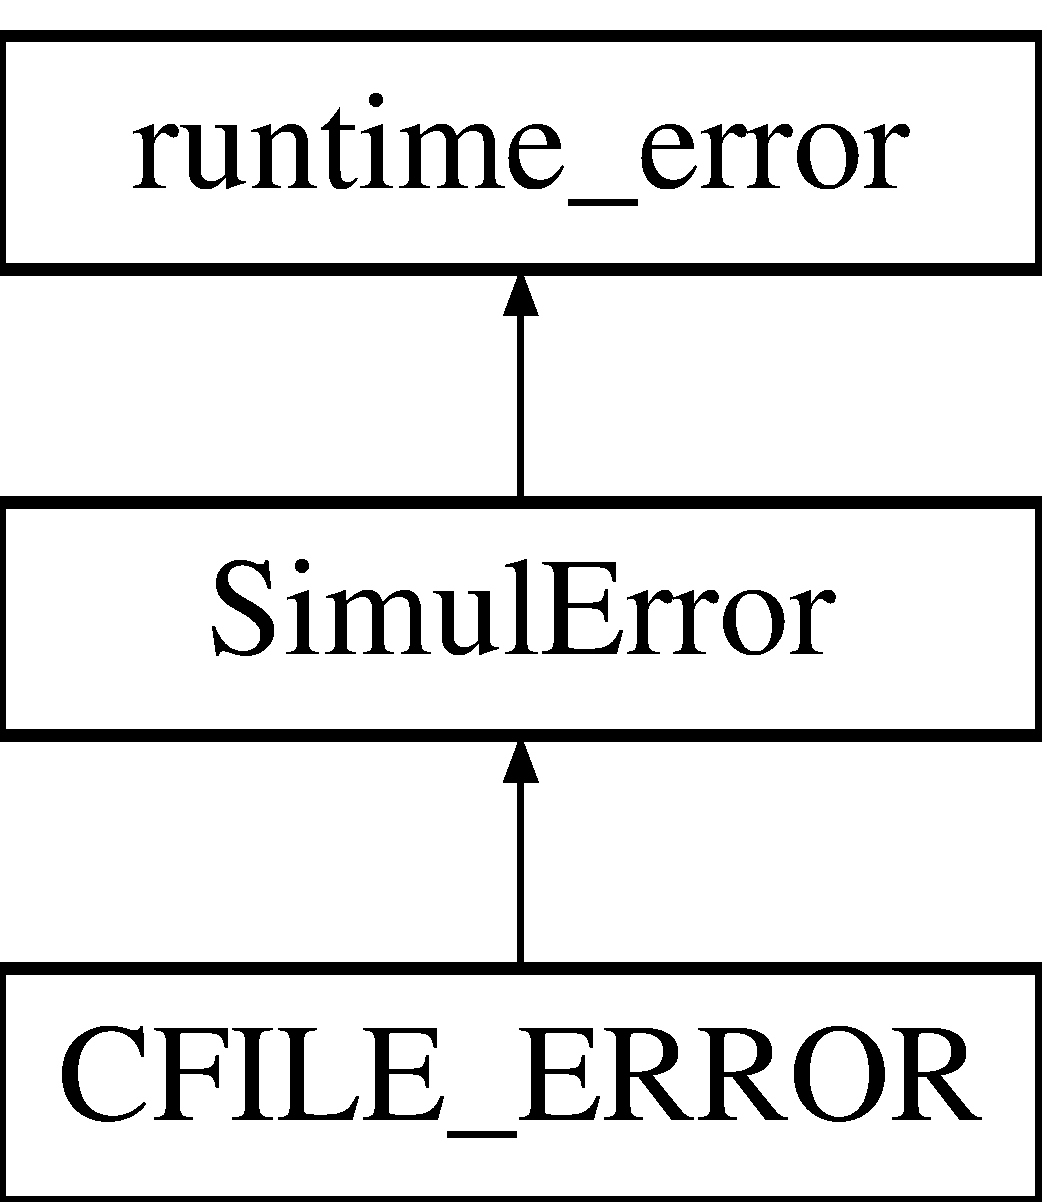
\includegraphics[height=3.000000cm]{classCFILE__ERROR}
\end{center}
\end{figure}
\subsection*{Public Member Functions}
\begin{DoxyCompactItemize}
\item 
\hyperlink{classCFILE__ERROR_abd14368fd5f3051baf336bbd24bab99f}{C\+F\+I\+L\+E\+\_\+\+E\+R\+R\+OR} (const char $\ast$c)
\item 
\hyperlink{classCFILE__ERROR_a20393787ce4998a586a518f0478de5f3}{C\+F\+I\+L\+E\+\_\+\+E\+R\+R\+OR} (const std\+::string \&s)
\end{DoxyCompactItemize}
\subsection*{Additional Inherited Members}


\subsection{Constructor \& Destructor Documentation}
\mbox{\Hypertarget{classCFILE__ERROR_abd14368fd5f3051baf336bbd24bab99f}\label{classCFILE__ERROR_abd14368fd5f3051baf336bbd24bab99f}} 
\index{C\+F\+I\+L\+E\+\_\+\+E\+R\+R\+OR@{C\+F\+I\+L\+E\+\_\+\+E\+R\+R\+OR}!C\+F\+I\+L\+E\+\_\+\+E\+R\+R\+OR@{C\+F\+I\+L\+E\+\_\+\+E\+R\+R\+OR}}
\index{C\+F\+I\+L\+E\+\_\+\+E\+R\+R\+OR@{C\+F\+I\+L\+E\+\_\+\+E\+R\+R\+OR}!C\+F\+I\+L\+E\+\_\+\+E\+R\+R\+OR@{C\+F\+I\+L\+E\+\_\+\+E\+R\+R\+OR}}
\subsubsection{\texorpdfstring{C\+F\+I\+L\+E\+\_\+\+E\+R\+R\+O\+R()}{CFILE\_ERROR()}\hspace{0.1cm}{\footnotesize\ttfamily [1/2]}}
{\footnotesize\ttfamily C\+F\+I\+L\+E\+\_\+\+E\+R\+R\+O\+R\+::\+C\+F\+I\+L\+E\+\_\+\+E\+R\+R\+OR (\begin{DoxyParamCaption}\item[{const char $\ast$}]{c }\end{DoxyParamCaption})\hspace{0.3cm}{\ttfamily [inline]}}


\begin{DoxyCode}
63 :0.4,CH:0.35\textcolor{stringliteral}{'. If total is less than 1, it will be completed with RS neurons"}
\end{DoxyCode}
\mbox{\Hypertarget{classCFILE__ERROR_a20393787ce4998a586a518f0478de5f3}\label{classCFILE__ERROR_a20393787ce4998a586a518f0478de5f3}} 
\index{C\+F\+I\+L\+E\+\_\+\+E\+R\+R\+OR@{C\+F\+I\+L\+E\+\_\+\+E\+R\+R\+OR}!C\+F\+I\+L\+E\+\_\+\+E\+R\+R\+OR@{C\+F\+I\+L\+E\+\_\+\+E\+R\+R\+OR}}
\index{C\+F\+I\+L\+E\+\_\+\+E\+R\+R\+OR@{C\+F\+I\+L\+E\+\_\+\+E\+R\+R\+OR}!C\+F\+I\+L\+E\+\_\+\+E\+R\+R\+OR@{C\+F\+I\+L\+E\+\_\+\+E\+R\+R\+OR}}
\subsubsection{\texorpdfstring{C\+F\+I\+L\+E\+\_\+\+E\+R\+R\+O\+R()}{CFILE\_ERROR()}\hspace{0.1cm}{\footnotesize\ttfamily [2/2]}}
{\footnotesize\ttfamily C\+F\+I\+L\+E\+\_\+\+E\+R\+R\+O\+R\+::\+C\+F\+I\+L\+E\+\_\+\+E\+R\+R\+OR (\begin{DoxyParamCaption}\item[{const std\+::string \&}]{s }\end{DoxyParamCaption})\hspace{0.3cm}{\ttfamily [inline]}}


\begin{DoxyCode}
63 :0.4,CH:0.35\textcolor{stringliteral}{'. If total is less than 1, it will be completed with RS neurons"}
\end{DoxyCode}


The documentation for this class was generated from the following file\+:\begin{DoxyCompactItemize}
\item 
/home/celio/myfiles/\+Programmation/semaine5/\+Neuron\+Net/src/\hyperlink{globals_8h}{globals.\+h}\end{DoxyCompactItemize}

\hypertarget{structSimulation_1_1intervalConstr}{}\section{Simulation\+:\+:interval\+Constr Struct Reference}
\label{structSimulation_1_1intervalConstr}\index{Simulation\+::interval\+Constr@{Simulation\+::interval\+Constr}}
Inheritance diagram for Simulation\+:\+:interval\+Constr\+:\begin{figure}[H]
\begin{center}
\leavevmode
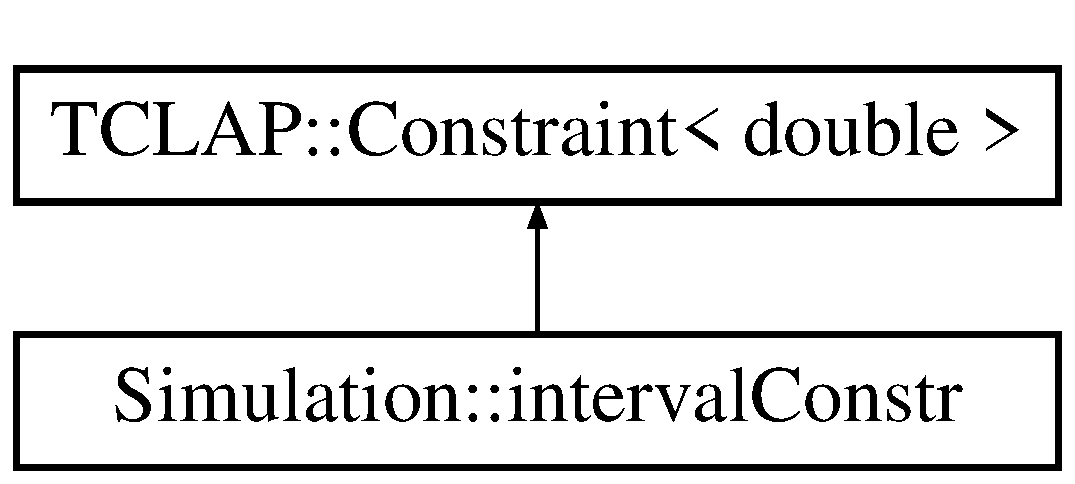
\includegraphics[height=2.000000cm]{structSimulation_1_1intervalConstr}
\end{center}
\end{figure}
\subsection*{Public Member Functions}
\begin{DoxyCompactItemize}
\item 
std\+::string \hyperlink{structSimulation_1_1intervalConstr_a100c7d32a4c1e571e15bbc7463fee2b2}{short\+ID} () const
\item 
std\+::string \hyperlink{structSimulation_1_1intervalConstr_acd0d4140e524a5017441f3d10ca9d3bf}{description} () const
\item 
bool \hyperlink{structSimulation_1_1intervalConstr_a7c2cbda337f9d4ef3a626019120a2316}{check} (const double \&x) const
\end{DoxyCompactItemize}


\subsection{Detailed Description}
Constraint function for a T\+C\+L\+AP argument to restrict a double to \mbox{[}0,1\mbox{]}. 

\subsection{Member Function Documentation}
\mbox{\Hypertarget{structSimulation_1_1intervalConstr_a7c2cbda337f9d4ef3a626019120a2316}\label{structSimulation_1_1intervalConstr_a7c2cbda337f9d4ef3a626019120a2316}} 
\index{Simulation\+::interval\+Constr@{Simulation\+::interval\+Constr}!check@{check}}
\index{check@{check}!Simulation\+::interval\+Constr@{Simulation\+::interval\+Constr}}
\subsubsection{\texorpdfstring{check()}{check()}}
{\footnotesize\ttfamily bool Simulation\+::interval\+Constr\+::check (\begin{DoxyParamCaption}\item[{const double \&}]{x }\end{DoxyParamCaption}) const\hspace{0.3cm}{\ttfamily [inline]}}


\begin{DoxyCode}
65 \{\textcolor{keywordflow}{return} (x >= 0) && (x <= 1);\}
\end{DoxyCode}
\mbox{\Hypertarget{structSimulation_1_1intervalConstr_acd0d4140e524a5017441f3d10ca9d3bf}\label{structSimulation_1_1intervalConstr_acd0d4140e524a5017441f3d10ca9d3bf}} 
\index{Simulation\+::interval\+Constr@{Simulation\+::interval\+Constr}!description@{description}}
\index{description@{description}!Simulation\+::interval\+Constr@{Simulation\+::interval\+Constr}}
\subsubsection{\texorpdfstring{description()}{description()}}
{\footnotesize\ttfamily std\+::string Simulation\+::interval\+Constr\+::description (\begin{DoxyParamCaption}{ }\end{DoxyParamCaption}) const\hspace{0.3cm}{\ttfamily [inline]}}


\begin{DoxyCode}
64 \{\textcolor{keywordflow}{return} \textcolor{stringliteral}{"A number in [0,1]"};\}
\end{DoxyCode}
\mbox{\Hypertarget{structSimulation_1_1intervalConstr_a100c7d32a4c1e571e15bbc7463fee2b2}\label{structSimulation_1_1intervalConstr_a100c7d32a4c1e571e15bbc7463fee2b2}} 
\index{Simulation\+::interval\+Constr@{Simulation\+::interval\+Constr}!short\+ID@{short\+ID}}
\index{short\+ID@{short\+ID}!Simulation\+::interval\+Constr@{Simulation\+::interval\+Constr}}
\subsubsection{\texorpdfstring{short\+I\+D()}{shortID()}}
{\footnotesize\ttfamily std\+::string Simulation\+::interval\+Constr\+::short\+ID (\begin{DoxyParamCaption}{ }\end{DoxyParamCaption}) const\hspace{0.3cm}{\ttfamily [inline]}}


\begin{DoxyCode}
63 \{\textcolor{keywordflow}{return} \textcolor{stringliteral}{"[0,1]"};\}
\end{DoxyCode}


The documentation for this struct was generated from the following file\+:\begin{DoxyCompactItemize}
\item 
/home/celio/myfiles/\+Programmation/semaine5/\+Neuron\+Net/src/\hyperlink{simulation_8h}{simulation.\+h}\end{DoxyCompactItemize}

\hypertarget{classNetwork}{}\section{Network Class Reference}
\label{classNetwork}\index{Network@{Network}}


{\ttfamily \#include $<$network.\+h$>$}

\subsection*{Public Member Functions}
\begin{DoxyCompactItemize}
\item 
void \hyperlink{classNetwork_ad91ae24f308dd2b46ff76396fcdb9765}{resize} (const size\+\_\+t \&, double \+\_\+i=0.\+2)
\item 
void \hyperlink{classNetwork_ad1d20020028425cfab199da1942172c9}{set\+\_\+default\+\_\+params} (const std\+::map$<$ std\+::string, size\+\_\+t $>$ \&, const size\+\_\+t \+\_\+s=0)
\item 
void \hyperlink{classNetwork_a40daf6578a6146f4c339f0efffd5070d}{set\+\_\+types\+\_\+params} (const std\+::vector$<$ std\+::string $>$ \&, const std\+::vector$<$ \hyperlink{structNeuronParams}{Neuron\+Params} $>$ \&, const size\+\_\+t \+\_\+s=0)
\item 
void \hyperlink{classNetwork_a699416a6462f2da6a5f6cddb30f31440}{set\+\_\+values} (const std\+::vector$<$ double $>$ \&, const size\+\_\+t \+\_\+s=0)
\item 
bool \hyperlink{classNetwork_a6ebe0899329973e4924997a25e205856}{add\+\_\+link} (const size\+\_\+t \&, const size\+\_\+t \&, double)
\item 
size\+\_\+t \hyperlink{classNetwork_a681d8f731ce258376a20f9bf062b943b}{random\+\_\+connect} (const double \&, const double \&s=.\+25)
\item 
size\+\_\+t \hyperlink{classNetwork_a41c54d12d861883170b5c5abca3a7bc8}{size} () const
\item 
std\+::pair$<$ size\+\_\+t, double $>$ \hyperlink{classNetwork_a06de035ba134c5aed590bd5f9f8035d1}{degree} (const size\+\_\+t \&index) const
\item 
const \hyperlink{classNeuron}{Neuron} \& \hyperlink{classNetwork_a4639c4fd24bc6dc807ae35af6577ed7f}{neuron} (const size\+\_\+t n) const
\item 
std\+::vector$<$ std\+::pair$<$ size\+\_\+t, double $>$ $>$ \hyperlink{classNetwork_abf7324fe99e691cb9b06247e5e5013fd}{neighbors} (const size\+\_\+t \&index) const
\item 
std\+::vector$<$ double $>$ \hyperlink{classNetwork_a44d9c341bfec26cb37efe3c29fd7a103}{potentials} () const
\item 
std\+::vector$<$ double $>$ \hyperlink{classNetwork_a2e9dbb815c622cccdd50186ae8c9f4a7}{recoveries} () const
\item 
std\+::set$<$ size\+\_\+t $>$ \hyperlink{classNetwork_a4614f267a2238b8a10dfea23b54defac}{step} (const std\+::vector$<$ double $>$ \&thalam)
\item 
void \hyperlink{classNetwork_afc43116eb2429aeec0f3c6a54d252142}{print\+\_\+params} (std\+::ostream $\ast$\+\_\+out=\&std\+::cout)
\item 
void \hyperlink{classNetwork_ae460d31557bba058fdf66e4fe5feb801}{print\+\_\+traj} (const int, const std\+::map$<$ std\+::string, size\+\_\+t $>$ \&, std\+::ostream $\ast$\+\_\+out=\&std\+::cout)
\item 
void \hyperlink{classNetwork_ab572dd33cb91d9f0aae89c4477809d26}{print\+\_\+head} (const std\+::map$<$ std\+::string, size\+\_\+t $>$ \&, std\+::ostream $\ast$\+\_\+out=\&std\+::cout)
\end{DoxyCompactItemize}
\subsection*{Private Attributes}
\begin{DoxyCompactItemize}
\item 
std\+::vector$<$ \hyperlink{classNeuron}{Neuron} $>$ \hyperlink{classNetwork_a1b7832bc2c7b8855cdc3b2d6329eff9d}{neurons}
\item 
\hyperlink{network_8h_a889f48bcec09c9d72a03648e911c5ff5}{linkmap} \hyperlink{classNetwork_aef1609a9a6b865651417ce995b4575a8}{links}
\end{DoxyCompactItemize}


\subsection{Detailed Description}
A neuron network is a \hyperlink{classNetwork_a1b7832bc2c7b8855cdc3b2d6329eff9d}{set} of neurons and a \hyperlink{classNetwork_aef1609a9a6b865651417ce995b4575a8}{set} of directional links between them.

Neurons are objects of class \hyperlink{classNeuron}{Neuron} (they are identified by their index in the vector \hyperlink{classNetwork_a1b7832bc2c7b8855cdc3b2d6329eff9d}{neurons}). A link is an ordered pair of indices in \hyperlink{classNetwork_a1b7832bc2c7b8855cdc3b2d6329eff9d}{neurons} with an intensity value, collected in a \hyperlink{network_8h_a889f48bcec09c9d72a03648e911c5ff5}{linkmap}. This is a \href{https://en.cppreference.com/w/cpp/container/map}{\tt std\+::map} therefore only one connection can exist between two neurons.

To create a network, you need to \hyperlink{classNetwork_ad91ae24f308dd2b46ff76396fcdb9765}{resize} it and optionally \hyperlink{classNetwork_ad1d20020028425cfab199da1942172c9}{set\+\_\+default\+\_\+params} for each neuron. Then you can either call \hyperlink{classNetwork_a6ebe0899329973e4924997a25e205856}{add\+\_\+link} for each connection or generate a random network with \hyperlink{classNetwork_a681d8f731ce258376a20f9bf062b943b}{random\+\_\+connect}.

The dynamics of the network proceeds by calling \hyperlink{classNetwork_a4614f267a2238b8a10dfea23b54defac}{step}. The state of the network can be printed to output streams with \hyperlink{classNetwork_afc43116eb2429aeec0f3c6a54d252142}{print\+\_\+params} (to print all parameters of all neurons), \hyperlink{classNetwork_ae460d31557bba058fdf66e4fe5feb801}{print\+\_\+traj} to print the full state of one neuron of each type. The helper function \hyperlink{classNetwork_ab572dd33cb91d9f0aae89c4477809d26}{print\+\_\+head} will print a header line with the variable names for the the \hyperlink{classNetwork_ae460d31557bba058fdf66e4fe5feb801}{print\+\_\+traj} lines.

This class provides accessors to the following \hyperlink{classNeuron}{Neuron} properties
\begin{DoxyItemize}
\item \hyperlink{classNetwork_a06de035ba134c5aed590bd5f9f8035d1}{degree} \+: returns the degree of a neuron (number of incoming connections) and valence (sum of weights of these links)
\item \hyperlink{classNetwork_abf7324fe99e691cb9b06247e5e5013fd}{neighbors} \+: returns the indices of neurons with incoming links to a given neuron,
\item \hyperlink{classNetwork_a44d9c341bfec26cb37efe3c29fd7a103}{potentials} \+: returns the values of membrane potentials for all neurons,
\item \hyperlink{classNetwork_a2e9dbb815c622cccdd50186ae8c9f4a7}{recoveries} \+: returns the values of recovery variables for all neurons,
\item \hyperlink{classNetwork_a4639c4fd24bc6dc807ae35af6577ed7f}{neuron} \+: returns a const reference to a given neuron object. 
\end{DoxyItemize}

\subsection{Member Function Documentation}
\mbox{\Hypertarget{classNetwork_a6ebe0899329973e4924997a25e205856}\label{classNetwork_a6ebe0899329973e4924997a25e205856}} 
\index{Network@{Network}!add\+\_\+link@{add\+\_\+link}}
\index{add\+\_\+link@{add\+\_\+link}!Network@{Network}}
\subsubsection{\texorpdfstring{add\+\_\+link()}{add\_link()}}
{\footnotesize\ttfamily bool Network\+::add\+\_\+link (\begin{DoxyParamCaption}\item[{const size\+\_\+t \&}]{a,  }\item[{const size\+\_\+t \&}]{b,  }\item[{double}]{str }\end{DoxyParamCaption})}

Creates a new link in \hyperlink{classNetwork_aef1609a9a6b865651417ce995b4575a8}{links}. 
\begin{DoxyParams}{Parameters}
{\em a} & (size\+\_\+t)\+: receiving neuron, \\
\hline
{\em b} & (size\+\_\+t)\+: sending neuron, \\
\hline
{\em str} & (double)\+: link intensity (will be multiplied by -\/2 for inhibitory source). \\
\hline
\end{DoxyParams}
\begin{DoxyReturn}{Returns}
true if the link could be created. 
\end{DoxyReturn}

\begin{DoxyCode}
38                                                                    \{
39     \textcolor{keywordflow}{if} (a==b || a>=\hyperlink{classNetwork_a41c54d12d861883170b5c5abca3a7bc8}{size}() || b>=\hyperlink{classNetwork_a41c54d12d861883170b5c5abca3a7bc8}{size}() || str<1e-6) \textcolor{keywordflow}{return} \textcolor{keyword}{false};
40     \textcolor{keywordflow}{if} (\hyperlink{classNetwork_aef1609a9a6b865651417ce995b4575a8}{links}.count(\{a,b\})) \textcolor{keywordflow}{return} \textcolor{keyword}{false};
41     \textcolor{keywordflow}{if} (\hyperlink{classNetwork_a1b7832bc2c7b8855cdc3b2d6329eff9d}{neurons}[b].is\_inhibitory()) str *= -2.0;
42     \hyperlink{classNetwork_aef1609a9a6b865651417ce995b4575a8}{links}.insert(\{\{a,b\}, str\});
43     \textcolor{keywordflow}{return} \textcolor{keyword}{true};
44 \}
\end{DoxyCode}
\mbox{\Hypertarget{classNetwork_a06de035ba134c5aed590bd5f9f8035d1}\label{classNetwork_a06de035ba134c5aed590bd5f9f8035d1}} 
\index{Network@{Network}!degree@{degree}}
\index{degree@{degree}!Network@{Network}}
\subsubsection{\texorpdfstring{degree()}{degree()}}
{\footnotesize\ttfamily std\+::pair$<$ size\+\_\+t, double $>$ Network\+::degree (\begin{DoxyParamCaption}\item[{const size\+\_\+t \&}]{index }\end{DoxyParamCaption}) const}

Calculates the number and total intensity of connections to neuron {\ttfamily n}. 
\begin{DoxyParams}{Parameters}
{\em n} & \+: the index of the receiving neuron. \\
\hline
\end{DoxyParams}
\begin{DoxyReturn}{Returns}
a pair \{number of connections, sum of link intensities\}. 
\end{DoxyReturn}
\{neuron index, link intensity\} 
\begin{DoxyCode}
134 \{
135     std::vector<std::pair<size\_t, double> > connections(\hyperlink{classNetwork_abf7324fe99e691cb9b06247e5e5013fd}{neighbors}(index));
137     \textcolor{keywordtype}{double} sum;
138 
139     \textcolor{keywordflow}{for} (\textcolor{keyword}{auto} n : connections) \{
140         sum += n.second;
141     \}
142     
143     \textcolor{keywordflow}{return} \{connections.size(), sum\};
144 \}
\end{DoxyCode}
\mbox{\Hypertarget{classNetwork_abf7324fe99e691cb9b06247e5e5013fd}\label{classNetwork_abf7324fe99e691cb9b06247e5e5013fd}} 
\index{Network@{Network}!neighbors@{neighbors}}
\index{neighbors@{neighbors}!Network@{Network}}
\subsubsection{\texorpdfstring{neighbors()}{neighbors()}}
{\footnotesize\ttfamily std\+::vector$<$ std\+::pair$<$ size\+\_\+t, double $>$ $>$ Network\+::neighbors (\begin{DoxyParamCaption}\item[{const size\+\_\+t \&}]{index }\end{DoxyParamCaption}) const}

Finds the list of neurons with incoming connections to {\ttfamily n}. 
\begin{DoxyParams}{Parameters}
{\em n} & \+: the index of the receiving neuron. \\
\hline
\end{DoxyParams}
\begin{DoxyReturn}{Returns}
a vector of pairs \{neuron index, link intensity\}. 
\end{DoxyReturn}

\begin{DoxyCode}
147 \{
148     std::vector<std::pair<size\_t, double> > \hyperlink{classNetwork_abf7324fe99e691cb9b06247e5e5013fd}{neighbors};
149     \textcolor{comment}{/*for (auto c : links) \{}
150 \textcolor{comment}{        if((c.first).first == index) \{}
151 \textcolor{comment}{            neighbors.push\_back(\{(c.first).second, c.second\});}
152 \textcolor{comment}{        \}}
153 \textcolor{comment}{    \}}
154 \textcolor{comment}{    */}
155     \textcolor{keywordflow}{for}(std::map<std::pair<size\_t,size\_t>, \textcolor{keywordtype}{double}>::const\_iterator i=\hyperlink{classNetwork_aef1609a9a6b865651417ce995b4575a8}{links}.lower\_bound(\{index,0\});
156     i != \hyperlink{classNetwork_aef1609a9a6b865651417ce995b4575a8}{links}.end() and (i->first).first == index; i++)\{
157         neighbors.push\_back(\{(i->first).second, i->second\});
158     \}
159     \textcolor{keywordflow}{return} \hyperlink{classNetwork_abf7324fe99e691cb9b06247e5e5013fd}{neighbors};
160 \}
\end{DoxyCode}
\mbox{\Hypertarget{classNetwork_a4639c4fd24bc6dc807ae35af6577ed7f}\label{classNetwork_a4639c4fd24bc6dc807ae35af6577ed7f}} 
\index{Network@{Network}!neuron@{neuron}}
\index{neuron@{neuron}!Network@{Network}}
\subsubsection{\texorpdfstring{neuron()}{neuron()}}
{\footnotesize\ttfamily const \hyperlink{classNeuron}{Neuron}\& Network\+::neuron (\begin{DoxyParamCaption}\item[{const size\+\_\+t}]{n }\end{DoxyParamCaption}) const\hspace{0.3cm}{\ttfamily [inline]}}


\begin{DoxyCode}
83 \{\textcolor{keywordflow}{return} \hyperlink{classNetwork_a1b7832bc2c7b8855cdc3b2d6329eff9d}{neurons}.at(n);\}
\end{DoxyCode}
\mbox{\Hypertarget{classNetwork_a44d9c341bfec26cb37efe3c29fd7a103}\label{classNetwork_a44d9c341bfec26cb37efe3c29fd7a103}} 
\index{Network@{Network}!potentials@{potentials}}
\index{potentials@{potentials}!Network@{Network}}
\subsubsection{\texorpdfstring{potentials()}{potentials()}}
{\footnotesize\ttfamily std\+::vector$<$ double $>$ Network\+::potentials (\begin{DoxyParamCaption}{ }\end{DoxyParamCaption}) const}


\begin{DoxyCode}
65                                             \{
66     std::vector<double> vals;
67     \textcolor{keywordflow}{for} (\textcolor{keywordtype}{size\_t} nn=0; nn<\hyperlink{classNetwork_a41c54d12d861883170b5c5abca3a7bc8}{size}(); nn++)
68         vals.push\_back(\hyperlink{classNetwork_a1b7832bc2c7b8855cdc3b2d6329eff9d}{neurons}[nn].potential());
69     \textcolor{keywordflow}{return} vals;
70 \}
\end{DoxyCode}
\mbox{\Hypertarget{classNetwork_ab572dd33cb91d9f0aae89c4477809d26}\label{classNetwork_ab572dd33cb91d9f0aae89c4477809d26}} 
\index{Network@{Network}!print\+\_\+head@{print\+\_\+head}}
\index{print\+\_\+head@{print\+\_\+head}!Network@{Network}}
\subsubsection{\texorpdfstring{print\+\_\+head()}{print\_head()}}
{\footnotesize\ttfamily void Network\+::print\+\_\+head (\begin{DoxyParamCaption}\item[{const std\+::map$<$ std\+::string, size\+\_\+t $>$ \&}]{\+\_\+nt,  }\item[{std\+::ostream $\ast$}]{\+\_\+out = {\ttfamily \&std\+:\+:cout} }\end{DoxyParamCaption})}


\begin{DoxyCode}
90                                            \{
91     \textcolor{keywordtype}{size\_t} total = 0;
92     \textcolor{keywordflow}{for} (\textcolor{keyword}{auto} It : \_nt) \{
93         total += It.second;
94         \textcolor{keywordflow}{for} (\textcolor{keyword}{auto} In : \hyperlink{classNetwork_a1b7832bc2c7b8855cdc3b2d6329eff9d}{neurons})
95             \textcolor{keywordflow}{if} (In.is\_type(It.first)) \{
96                 (*\_out) << \textcolor{charliteral}{'\(\backslash\)t'} << It.first << \textcolor{stringliteral}{".v"}
97                         << \textcolor{charliteral}{'\(\backslash\)t'} << It.first << \textcolor{stringliteral}{".u"}
98                         << \textcolor{charliteral}{'\(\backslash\)t'} << It.first << \textcolor{stringliteral}{".I"};
99                 \textcolor{keywordflow}{break};
100             \}
101     \}
102     \textcolor{keywordflow}{if} (total<\hyperlink{classNetwork_a41c54d12d861883170b5c5abca3a7bc8}{size}())
103         \textcolor{keywordflow}{for} (\textcolor{keyword}{auto} In : neurons) 
104             \textcolor{keywordflow}{if} (In.is\_type(\textcolor{stringliteral}{"RS"})) \{
105                 (*\_out) << \textcolor{charliteral}{'\(\backslash\)t'} << \textcolor{stringliteral}{"RS.v"} << \textcolor{charliteral}{'\(\backslash\)t'} << \textcolor{stringliteral}{"RS.u"} << \textcolor{charliteral}{'\(\backslash\)t'} << \textcolor{stringliteral}{"RS.I"};
106                 \textcolor{keywordflow}{break};
107             \}
108     (*\_out) << std::endl;
109 \}
\end{DoxyCode}
\mbox{\Hypertarget{classNetwork_afc43116eb2429aeec0f3c6a54d252142}\label{classNetwork_afc43116eb2429aeec0f3c6a54d252142}} 
\index{Network@{Network}!print\+\_\+params@{print\+\_\+params}}
\index{print\+\_\+params@{print\+\_\+params}!Network@{Network}}
\subsubsection{\texorpdfstring{print\+\_\+params()}{print\_params()}}
{\footnotesize\ttfamily void Network\+::print\+\_\+params (\begin{DoxyParamCaption}\item[{std\+::ostream $\ast$}]{\+\_\+out = {\ttfamily \&std\+:\+:cout} }\end{DoxyParamCaption})}


\begin{DoxyCode}
79                                            \{
80     (*\_out) << \textcolor{stringliteral}{"Type\(\backslash\)ta\(\backslash\)tb\(\backslash\)tc\(\backslash\)td\(\backslash\)tInhibitory\(\backslash\)tdegree\(\backslash\)tvalence"} << std::endl;
81     \textcolor{keywordflow}{for} (\textcolor{keywordtype}{size\_t} nn=0; nn<\hyperlink{classNetwork_a41c54d12d861883170b5c5abca3a7bc8}{size}(); nn++) \{
82         std::pair<size\_t, double> dI = \hyperlink{classNetwork_a06de035ba134c5aed590bd5f9f8035d1}{degree}(nn);
83         (*\_out) << \hyperlink{classNetwork_a1b7832bc2c7b8855cdc3b2d6329eff9d}{neurons}[nn].formatted\_params() 
84                 << \textcolor{charliteral}{'\(\backslash\)t'} << dI.first << \textcolor{charliteral}{'\(\backslash\)t'} << dI.second
85                 << std::endl;
86     \}
87 \}
\end{DoxyCode}
\mbox{\Hypertarget{classNetwork_ae460d31557bba058fdf66e4fe5feb801}\label{classNetwork_ae460d31557bba058fdf66e4fe5feb801}} 
\index{Network@{Network}!print\+\_\+traj@{print\+\_\+traj}}
\index{print\+\_\+traj@{print\+\_\+traj}!Network@{Network}}
\subsubsection{\texorpdfstring{print\+\_\+traj()}{print\_traj()}}
{\footnotesize\ttfamily void Network\+::print\+\_\+traj (\begin{DoxyParamCaption}\item[{const int}]{time,  }\item[{const std\+::map$<$ std\+::string, size\+\_\+t $>$ \&}]{\+\_\+nt,  }\item[{std\+::ostream $\ast$}]{\+\_\+out = {\ttfamily \&std\+:\+:cout} }\end{DoxyParamCaption})}


\begin{DoxyCode}
112                                            \{
113     (*\_out)  << time;
114     \textcolor{keywordtype}{size\_t} total = 0;
115     \textcolor{keywordflow}{for} (\textcolor{keyword}{auto} It : \_nt) \{
116         total += It.second;
117         \textcolor{keywordflow}{for} (\textcolor{keyword}{auto} In : \hyperlink{classNetwork_a1b7832bc2c7b8855cdc3b2d6329eff9d}{neurons}) 
118             \textcolor{keywordflow}{if} (In.is\_type(It.first)) \{
119                 (*\_out) << \textcolor{charliteral}{'\(\backslash\)t'} << In.formatted\_values();
120                 \textcolor{keywordflow}{break};
121             \}
122     \}
123     \textcolor{keywordflow}{if} (total<\hyperlink{classNetwork_a41c54d12d861883170b5c5abca3a7bc8}{size}())
124         \textcolor{keywordflow}{for} (\textcolor{keyword}{auto} In : neurons) 
125             \textcolor{keywordflow}{if} (In.is\_type(\textcolor{stringliteral}{"RS"})) \{
126                 (*\_out) << \textcolor{charliteral}{'\(\backslash\)t'} << In.formatted\_values();
127                 \textcolor{keywordflow}{break};
128             \}
129     (*\_out) << std::endl;
130 \}
\end{DoxyCode}
\mbox{\Hypertarget{classNetwork_a681d8f731ce258376a20f9bf062b943b}\label{classNetwork_a681d8f731ce258376a20f9bf062b943b}} 
\index{Network@{Network}!random\+\_\+connect@{random\+\_\+connect}}
\index{random\+\_\+connect@{random\+\_\+connect}!Network@{Network}}
\subsubsection{\texorpdfstring{random\+\_\+connect()}{random\_connect()}}
{\footnotesize\ttfamily size\+\_\+t Network\+::random\+\_\+connect (\begin{DoxyParamCaption}\item[{const double \&}]{mean\+\_\+deg,  }\item[{const double \&}]{s = {\ttfamily .25} }\end{DoxyParamCaption})}

Creates random links in the network. Each neuron will expect to receive {\itshape n} connections (\hyperlink{classRandomNumbers_a1195251686ad00cd782c9a91a44d983b}{Random\+Numbers\+::poisson} with mean {\ttfamily mean\+\_\+deg}) of intensity {\itshape s} (\hyperlink{classRandomNumbers_ae226c129494f9055ac37ed1af943d010}{Random\+Numbers\+::uniform\+\_\+double} with mean {\ttfamily mean\+\_\+streng}). Sending neurons will be picked at random and since there can be only one connection from each neuron, the expected degree is not always achieved. 
\begin{DoxyParams}{Parameters}
{\em mean\+\_\+deg} & (double)\+: mean value of Poisson distribution. \\
\hline
{\em mean\+\_\+streng} & (double)\+: mean value of the uniform distribution (with bounds 0 and 2$\ast$mean\+\_\+streng). \\
\hline
\end{DoxyParams}
\begin{DoxyReturn}{Returns}
the number of links created. 
\end{DoxyReturn}

\begin{DoxyCode}
46                                                                                 \{
47     \hyperlink{classNetwork_aef1609a9a6b865651417ce995b4575a8}{links}.clear();
48     std::vector<int> degrees(\hyperlink{classNetwork_a41c54d12d861883170b5c5abca3a7bc8}{size}());
49     \hyperlink{main_8cpp_ad20d7a8b3940b60cfd9cd7188fb503ea}{\_RNG}->\hyperlink{classRandomNumbers_a1195251686ad00cd782c9a91a44d983b}{poisson}(degrees, mean\_deg);
50     \textcolor{keywordtype}{size\_t} num\_links = 0;
51     std::vector<size\_t> nodeidx(\hyperlink{classNetwork_a41c54d12d861883170b5c5abca3a7bc8}{size}());
52     std::iota(nodeidx.begin(), nodeidx.end(), 0);
53     \textcolor{keywordflow}{for} (\textcolor{keywordtype}{size\_t} node=0; node<\hyperlink{classNetwork_a41c54d12d861883170b5c5abca3a7bc8}{size}(); node++) \{
54         \hyperlink{main_8cpp_ad20d7a8b3940b60cfd9cd7188fb503ea}{\_RNG}->\hyperlink{classRandomNumbers_a851aaa7e46922dc22ce984b21b474a4e}{shuffle}(nodeidx);
55         std::vector<double> strength(degrees[node]);
56         \hyperlink{main_8cpp_ad20d7a8b3940b60cfd9cd7188fb503ea}{\_RNG}->\hyperlink{classRandomNumbers_ae226c129494f9055ac37ed1af943d010}{uniform\_double}(strength, 1e-6, 2*mean\_streng);
57         \textcolor{keywordtype}{int} nl = 0;
58         \textcolor{keywordflow}{for} (\textcolor{keywordtype}{size\_t} nn=0; nn<\hyperlink{classNetwork_a41c54d12d861883170b5c5abca3a7bc8}{size}() && nl<degrees[node]; nn++)
59             \textcolor{keywordflow}{if} (\hyperlink{classNetwork_a6ebe0899329973e4924997a25e205856}{add\_link}(node, nodeidx[nn], strength[nl])) nl++;
60         num\_links += nl;
61     \}
62     \textcolor{keywordflow}{return} num\_links;
63 \}
\end{DoxyCode}
\mbox{\Hypertarget{classNetwork_a2e9dbb815c622cccdd50186ae8c9f4a7}\label{classNetwork_a2e9dbb815c622cccdd50186ae8c9f4a7}} 
\index{Network@{Network}!recoveries@{recoveries}}
\index{recoveries@{recoveries}!Network@{Network}}
\subsubsection{\texorpdfstring{recoveries()}{recoveries()}}
{\footnotesize\ttfamily std\+::vector$<$ double $>$ Network\+::recoveries (\begin{DoxyParamCaption}{ }\end{DoxyParamCaption}) const}


\begin{DoxyCode}
72                                             \{
73     std::vector<double> vals;
74     \textcolor{keywordflow}{for} (\textcolor{keywordtype}{size\_t} nn=0; nn<\hyperlink{classNetwork_a41c54d12d861883170b5c5abca3a7bc8}{size}(); nn++)
75         vals.push\_back(\hyperlink{classNetwork_a1b7832bc2c7b8855cdc3b2d6329eff9d}{neurons}[nn].recovery());
76     \textcolor{keywordflow}{return} vals;
77 \}
\end{DoxyCode}
\mbox{\Hypertarget{classNetwork_ad91ae24f308dd2b46ff76396fcdb9765}\label{classNetwork_ad91ae24f308dd2b46ff76396fcdb9765}} 
\index{Network@{Network}!resize@{resize}}
\index{resize@{resize}!Network@{Network}}
\subsubsection{\texorpdfstring{resize()}{resize()}}
{\footnotesize\ttfamily void Network\+::resize (\begin{DoxyParamCaption}\item[{const size\+\_\+t \&}]{n,  }\item[{double}]{\+\_\+i = {\ttfamily 0.2} }\end{DoxyParamCaption})}

Resizes a network (grow or shrink). 
\begin{DoxyParams}{Parameters}
{\em n} & (size\+\_\+t)\+: new size of the network. If growing it will be filled with default excitatory and inhibitory neurons. \\
\hline
{\em \+\_\+i} & (double)\+: proportion of inhibitory neurons among the newly created. \\
\hline
\end{DoxyParams}

\begin{DoxyCode}
4                                                   \{
5     \textcolor{keywordtype}{size\_t} old = \hyperlink{classNetwork_a41c54d12d861883170b5c5abca3a7bc8}{size}();
6     \hyperlink{classNetwork_a1b7832bc2c7b8855cdc3b2d6329eff9d}{neurons}.resize(n);
7     \textcolor{keywordflow}{if} (n <= old) \textcolor{keywordflow}{return};
8     \textcolor{keywordtype}{size\_t} nfs(inhib*(n-old)+.5);
9     \hyperlink{classNetwork_ad1d20020028425cfab199da1942172c9}{set\_default\_params}(\{\{\textcolor{stringliteral}{"FS"}, nfs\}\}, old);
10 \}
\end{DoxyCode}
\mbox{\Hypertarget{classNetwork_ad1d20020028425cfab199da1942172c9}\label{classNetwork_ad1d20020028425cfab199da1942172c9}} 
\index{Network@{Network}!set\+\_\+default\+\_\+params@{set\+\_\+default\+\_\+params}}
\index{set\+\_\+default\+\_\+params@{set\+\_\+default\+\_\+params}!Network@{Network}}
\subsubsection{\texorpdfstring{set\+\_\+default\+\_\+params()}{set\_default\_params()}}
{\footnotesize\ttfamily void Network\+::set\+\_\+default\+\_\+params (\begin{DoxyParamCaption}\item[{const std\+::map$<$ std\+::string, size\+\_\+t $>$ \&}]{types,  }\item[{const size\+\_\+t}]{\+\_\+s = {\ttfamily 0} }\end{DoxyParamCaption})}

Sets the neurons parameters. 
\begin{DoxyParams}{Parameters}
{\em \+\_\+types} & \+: a map between \hyperlink{classNeuron_ab4b47274e756b72923d2f8a9a5037d23}{Neuron\+::\+Neuron\+Types} and the number of neurons to set. \\
\hline
{\em \+\_\+s} & \+: neurons will be set consecutively in \hyperlink{classNetwork_a1b7832bc2c7b8855cdc3b2d6329eff9d}{neurons} starting from that index. \\
\hline
\end{DoxyParams}

\begin{DoxyCode}
13                                                      \{
14     \textcolor{keywordtype}{size\_t} k(0), ssize(\hyperlink{classNetwork_a41c54d12d861883170b5c5abca3a7bc8}{size}()-start), kmax(0);
15     std::vector<double> \hyperlink{test__main_8cpp_aedb3acb007b8cca8efc63eed08f45705}{noise}(ssize);
16     \hyperlink{main_8cpp_ad20d7a8b3940b60cfd9cd7188fb503ea}{\_RNG}->\hyperlink{classRandomNumbers_ae226c129494f9055ac37ed1af943d010}{uniform\_double}(\hyperlink{test__main_8cpp_aedb3acb007b8cca8efc63eed08f45705}{noise});
17     \textcolor{keywordflow}{for} (\textcolor{keyword}{auto} I : types) 
18         \textcolor{keywordflow}{if} (\hyperlink{classNeuron_a3a80c93e7cf5214b5e1a9925742bbe8e}{Neuron::type\_exists}(I.first)) 
19             \textcolor{keywordflow}{for} (kmax+=I.second; k<kmax && k<ssize; k++) 
20                 \hyperlink{classNetwork_a1b7832bc2c7b8855cdc3b2d6329eff9d}{neurons}[start+k].set\_default\_params(I.first, \hyperlink{test__main_8cpp_aedb3acb007b8cca8efc63eed08f45705}{noise}[k]);
21     \textcolor{keywordflow}{for} (; k<ssize; k++) \hyperlink{classNetwork_a1b7832bc2c7b8855cdc3b2d6329eff9d}{neurons}[start+k].\hyperlink{classNetwork_ad1d20020028425cfab199da1942172c9}{set\_default\_params}(\textcolor{stringliteral}{"RS"}, 
      \hyperlink{test__main_8cpp_aedb3acb007b8cca8efc63eed08f45705}{noise}[k]);
22 \}
\end{DoxyCode}
\mbox{\Hypertarget{classNetwork_a40daf6578a6146f4c339f0efffd5070d}\label{classNetwork_a40daf6578a6146f4c339f0efffd5070d}} 
\index{Network@{Network}!set\+\_\+types\+\_\+params@{set\+\_\+types\+\_\+params}}
\index{set\+\_\+types\+\_\+params@{set\+\_\+types\+\_\+params}!Network@{Network}}
\subsubsection{\texorpdfstring{set\+\_\+types\+\_\+params()}{set\_types\_params()}}
{\footnotesize\ttfamily void Network\+::set\+\_\+types\+\_\+params (\begin{DoxyParamCaption}\item[{const std\+::vector$<$ std\+::string $>$ \&}]{\+\_\+types,  }\item[{const std\+::vector$<$ \hyperlink{structNeuronParams}{Neuron\+Params} $>$ \&}]{\+\_\+par,  }\item[{const size\+\_\+t}]{\+\_\+s = {\ttfamily 0} }\end{DoxyParamCaption})}

Sets the neurons parameters to non-\/default values. 
\begin{DoxyParams}{Parameters}
{\em \+\_\+types} & \+: a vector of \hyperlink{classNeuron_ab4b47274e756b72923d2f8a9a5037d23}{Neuron\+::\+Neuron\+Types}. \\
\hline
{\em \+\_\+par} & \+: a vector of parameter values (\hyperlink{structNeuronParams}{Neuron\+Params}). \\
\hline
{\em \+\_\+start} & \+: index of starting neuron in \hyperlink{classNetwork_a1b7832bc2c7b8855cdc3b2d6329eff9d}{neurons}. \\
\hline
\end{DoxyParams}

\begin{DoxyCode}
26                                                    \{
27     \textcolor{keywordflow}{for} (\textcolor{keywordtype}{size\_t} k=0; k<\_par.size(); k++) \{
28         \hyperlink{classNetwork_a1b7832bc2c7b8855cdc3b2d6329eff9d}{neurons}[start+k].set\_type(\_types[k]);
29         \hyperlink{classNetwork_a1b7832bc2c7b8855cdc3b2d6329eff9d}{neurons}[start+k].set\_params(\_par[k]);
30     \}
31 \}
\end{DoxyCode}
\mbox{\Hypertarget{classNetwork_a699416a6462f2da6a5f6cddb30f31440}\label{classNetwork_a699416a6462f2da6a5f6cddb30f31440}} 
\index{Network@{Network}!set\+\_\+values@{set\+\_\+values}}
\index{set\+\_\+values@{set\+\_\+values}!Network@{Network}}
\subsubsection{\texorpdfstring{set\+\_\+values()}{set\_values()}}
{\footnotesize\ttfamily void Network\+::set\+\_\+values (\begin{DoxyParamCaption}\item[{const std\+::vector$<$ double $>$ \&}]{\+\_\+poten,  }\item[{const size\+\_\+t}]{\+\_\+s = {\ttfamily 0} }\end{DoxyParamCaption})}

Sets the values of all membrane potentials. 
\begin{DoxyParams}{Parameters}
{\em \+\_\+poten} & \+: a vector of potential \hyperlink{classNeuron_a7f7fdc3f9550b870351c60f618c11376}{Neuron\+::\+\_\+poten} values. \\
\hline
{\em \+\_\+s} & \+: index of starting neuron in \hyperlink{classNetwork_a1b7832bc2c7b8855cdc3b2d6329eff9d}{neurons}. \\
\hline
\end{DoxyParams}

\begin{DoxyCode}
33                                                                             \{
34     \textcolor{keywordflow}{for} (\textcolor{keywordtype}{size\_t} k=0; k<\_poten.size(); k++) 
35         \hyperlink{classNetwork_a1b7832bc2c7b8855cdc3b2d6329eff9d}{neurons}[start+k].potential(\_poten[k]);
36 \}
\end{DoxyCode}
\mbox{\Hypertarget{classNetwork_a41c54d12d861883170b5c5abca3a7bc8}\label{classNetwork_a41c54d12d861883170b5c5abca3a7bc8}} 
\index{Network@{Network}!size@{size}}
\index{size@{size}!Network@{Network}}
\subsubsection{\texorpdfstring{size()}{size()}}
{\footnotesize\ttfamily size\+\_\+t Network\+::size (\begin{DoxyParamCaption}{ }\end{DoxyParamCaption}) const\hspace{0.3cm}{\ttfamily [inline]}}


\begin{DoxyCode}
76 \{\textcolor{keywordflow}{return} \hyperlink{classNetwork_a1b7832bc2c7b8855cdc3b2d6329eff9d}{neurons}.size();\}
\end{DoxyCode}
\mbox{\Hypertarget{classNetwork_a4614f267a2238b8a10dfea23b54defac}\label{classNetwork_a4614f267a2238b8a10dfea23b54defac}} 
\index{Network@{Network}!step@{step}}
\index{step@{step}!Network@{Network}}
\subsubsection{\texorpdfstring{step()}{step()}}
{\footnotesize\ttfamily std\+::set$<$ size\+\_\+t $>$ Network\+::step (\begin{DoxyParamCaption}\item[{const std\+::vector$<$ double $>$ \&}]{thalam }\end{DoxyParamCaption})}

Performs one time-\/step of the simulation. 
\begin{DoxyParams}{Parameters}
{\em input} & \+: a vector of random values as thalamic input, one value for each neuron. The variance of these values corresponds to excitatory neurons. \\
\hline
\end{DoxyParams}
\begin{DoxyReturn}{Returns}
the indices of firing neurons. 
\end{DoxyReturn}

\begin{DoxyCode}
163 \{
164     std::set<size\_t> firing;
165     
166     \textcolor{keywordflow}{for}(\textcolor{keywordtype}{size\_t} i=0; i < \hyperlink{classNetwork_a1b7832bc2c7b8855cdc3b2d6329eff9d}{neurons}.size(); i++)\{
167         \textcolor{keywordflow}{if} (\hyperlink{classNetwork_a1b7832bc2c7b8855cdc3b2d6329eff9d}{neurons}[i].firing()) \{
168             \hyperlink{classNetwork_a1b7832bc2c7b8855cdc3b2d6329eff9d}{neurons}[i].reset();
169             firing.insert(i);
170             \}
171         \}
172     
173     \textcolor{keywordflow}{for} (\textcolor{keywordtype}{size\_t} i=0; i < \hyperlink{classNetwork_a1b7832bc2c7b8855cdc3b2d6329eff9d}{neurons}.size(); i++)\{
174         \textcolor{comment}{/*if (neurons[i].firing()) \{}
175 \textcolor{comment}{            neurons[i].reset();}
176 \textcolor{comment}{            \}}
177 \textcolor{comment}{            */}
178             
179         \textcolor{keywordtype}{double} w (0);
180         \textcolor{keywordtype}{double} I(0.);
181         \textcolor{keywordtype}{double} sum\_e(0.);
182         \textcolor{keywordtype}{double} sum\_i(0.);
183         std::vector<std::pair<size\_t, double> > connect(\hyperlink{classNetwork_abf7324fe99e691cb9b06247e5e5013fd}{neighbors}(i));
184         
185         \textcolor{keywordflow}{if}(\hyperlink{classNetwork_a1b7832bc2c7b8855cdc3b2d6329eff9d}{neurons}[i].is\_inhibitory()) \{w = 0.4;\}
186         \textcolor{keywordflow}{else} \{w = 1;\}
187         
188         \textcolor{keywordflow}{for} (\textcolor{keyword}{auto} neigh : connect) \{    
189             \textcolor{keywordflow}{if}(\hyperlink{classNetwork_a1b7832bc2c7b8855cdc3b2d6329eff9d}{neurons}[neigh.first].firing())\{ 
190                 \textcolor{keywordflow}{if} (\hyperlink{classNetwork_a1b7832bc2c7b8855cdc3b2d6329eff9d}{neurons}[neigh.first].is\_inhibitory()) \{sum\_i += neigh.second;\}
191                 \textcolor{keywordflow}{else} \{sum\_e += neigh.second;\}
192                 I = 0.5*(sum\_e)+sum\_i;
193             \}
194         \}
195 
196         I += thalam[i]*w;
197         \hyperlink{classNetwork_a1b7832bc2c7b8855cdc3b2d6329eff9d}{neurons}[i].input(I);
198         \hyperlink{classNetwork_a1b7832bc2c7b8855cdc3b2d6329eff9d}{neurons}[i].step();
199         \textcolor{comment}{/*if (neurons[i].firing()) \{}
200 \textcolor{comment}{            firing.insert(i);}
201 \textcolor{comment}{                        \}}
202 \textcolor{comment}{                        */}
203     \}
204         
205     \textcolor{keywordflow}{return} firing;
206 \}
\end{DoxyCode}


\subsection{Member Data Documentation}
\mbox{\Hypertarget{classNetwork_aef1609a9a6b865651417ce995b4575a8}\label{classNetwork_aef1609a9a6b865651417ce995b4575a8}} 
\index{Network@{Network}!links@{links}}
\index{links@{links}!Network@{Network}}
\subsubsection{\texorpdfstring{links}{links}}
{\footnotesize\ttfamily \hyperlink{network_8h_a889f48bcec09c9d72a03648e911c5ff5}{linkmap} Network\+::links\hspace{0.3cm}{\ttfamily [private]}}

\mbox{\Hypertarget{classNetwork_a1b7832bc2c7b8855cdc3b2d6329eff9d}\label{classNetwork_a1b7832bc2c7b8855cdc3b2d6329eff9d}} 
\index{Network@{Network}!neurons@{neurons}}
\index{neurons@{neurons}!Network@{Network}}
\subsubsection{\texorpdfstring{neurons}{neurons}}
{\footnotesize\ttfamily std\+::vector$<$\hyperlink{classNeuron}{Neuron}$>$ Network\+::neurons\hspace{0.3cm}{\ttfamily [private]}}



The documentation for this class was generated from the following files\+:\begin{DoxyCompactItemize}
\item 
/home/celio/myfiles/\+Programmation/semaine5/\+Neuron\+Net/src/\hyperlink{network_8h}{network.\+h}\item 
/home/celio/myfiles/\+Programmation/semaine5/\+Neuron\+Net/src/\hyperlink{network_8cpp}{network.\+cpp}\end{DoxyCompactItemize}

\hypertarget{classNeuron}{}\section{Neuron Class Reference}
\label{classNeuron}\index{Neuron@{Neuron}}


{\ttfamily \#include $<$neuron.\+h$>$}

\subsection*{Public Member Functions}
\begin{DoxyCompactItemize}
\item 
\hyperlink{classNeuron_a823487d01615fadb8ac19a2768dd9d96}{Neuron} ()
\item 
void \hyperlink{classNeuron_a85049e5f8745c53867178dd1cf6e51e3}{set\+\_\+params} (const \hyperlink{structNeuronParams}{Neuron\+Params} \&, const double n=0)
\item 
void \hyperlink{classNeuron_a533359bca915ef99c96e50d4bfff58b2}{set\+\_\+type} (std\+::string)
\item 
void \hyperlink{classNeuron_a0759d03a357708ee4174f1bbb2b0b8d7}{set\+\_\+default\+\_\+params} (const std\+::string \&, double n=0)
\item 
bool \hyperlink{classNeuron_a37459ba1dc4b0060707c33bf2ad5b10d}{is\+\_\+type} (const std\+::string \&)
\item 
std\+::string \hyperlink{classNeuron_abcf0b4ecd00cba630bfd2e764a61b5ee}{type} ()
\item 
bool \hyperlink{classNeuron_a649c6080b0749e6e642bf9df8f191d2d}{is\+\_\+inhibitory} () const
\item 
void \hyperlink{classNeuron_aa1481c474df55ad14373e51c6bb0f6fd}{set\+\_\+inhibitory} ()
\item 
bool \hyperlink{classNeuron_a4f477ebb623a7681c0f09dbfc4608a0d}{firing} () const
\item 
void \hyperlink{classNeuron_a6817fc5bf2128150b41b65e74f018408}{reset} ()
\item 
void \hyperlink{classNeuron_a224d5cead5f94bbe15ae49774db3e174}{step} ()
\item 
void \hyperlink{classNeuron_a47ea1a8f25dd62a34c9e0bdc0b7ae7fb}{potential} (const double \&\+\_\+p)
\item 
double \hyperlink{classNeuron_aab6607e17778ff1b4c05610c935b3156}{potential} () const
\item 
double \hyperlink{classNeuron_a2e84bc427827092295070dec404886f4}{recovery} () const
\item 
void \hyperlink{classNeuron_ab6b4f1a9633eaae9967cc6b226eed5fa}{input} (const double i)
\item 
double \hyperlink{classNeuron_ac00c31820b58e9c6f909db6a12e58b34}{input} () const
\end{DoxyCompactItemize}
\begin{Indent}\textbf{ Output strings}\par
{\em For printing purposes\+: all parameters and dynamic values are returned as a formatted string (tab-\/delimited concatenation of values). }\begin{DoxyCompactItemize}
\item 
std\+::string \hyperlink{classNeuron_a24dc0979745c7e25cfa997d88d973896}{formatted\+\_\+params} () const
\item 
std\+::string \hyperlink{classNeuron_aa1c46c99ed3e1a349b5e0ee82aec3026}{formatted\+\_\+values} () const
\end{DoxyCompactItemize}
\end{Indent}
\subsection*{Static Public Member Functions}
\begin{Indent}\textbf{ Static helpers}\par
{\em \hyperlink{classNeuron_a3a80c93e7cf5214b5e1a9925742bbe8e}{type\+\_\+exists} checks if the string {\ttfamily s} exists in the map \hyperlink{classNeuron_ab4b47274e756b72923d2f8a9a5037d23}{Neuron\+Types} and \hyperlink{classNeuron_a4e5c4e0a512460dd59449a0bec4d0db7}{type\+\_\+default} returns the corresponding \hyperlink{structNeuronParams}{Neuron\+Params} from \hyperlink{classNeuron_ab4b47274e756b72923d2f8a9a5037d23}{Neuron\+Types}. }\begin{DoxyCompactItemize}
\item 
static bool \hyperlink{classNeuron_a3a80c93e7cf5214b5e1a9925742bbe8e}{type\+\_\+exists} (const std\+::string \&s)
\item 
static \hyperlink{structNeuronParams}{Neuron\+Params} \hyperlink{classNeuron_a4e5c4e0a512460dd59449a0bec4d0db7}{type\+\_\+default} (const std\+::string \&s)
\end{DoxyCompactItemize}
\end{Indent}
\subsection*{Private Attributes}
\begin{Indent}\textbf{ Neuron parameters}\par
{\em {\ttfamily a}, {\ttfamily b}, {\ttfamily c}, {\ttfamily d}, and the boolean {\ttfamily inhib} if neuron is inhibitory. }\begin{DoxyCompactItemize}
\item 
\hyperlink{structNeuronParams}{Neuron\+Params} \hyperlink{classNeuron_a9427965b6669c7c35c327689de7a4d63}{params}
\end{DoxyCompactItemize}
\end{Indent}
\begin{Indent}\textbf{ Reference to the neuron type}\par
{\em This is an iterator to the relevant element of \hyperlink{classNeuron_ab4b47274e756b72923d2f8a9a5037d23}{Neuron\+::\+Neuron\+Types}. }\begin{DoxyCompactItemize}
\item 
std\+::map$<$ std\+::string, \hyperlink{structNeuronParams}{Neuron\+Params} $>$\+::const\+\_\+iterator \hyperlink{classNeuron_af48de7c2ad739fc5d57bfa2f3b1f7663}{\+\_\+type}
\end{DoxyCompactItemize}
\end{Indent}
\begin{Indent}\textbf{ Dynamic variables}\par
\begin{DoxyCompactItemize}
\item 
double \hyperlink{classNeuron_a7f7fdc3f9550b870351c60f618c11376}{\+\_\+poten}
\item 
double \hyperlink{classNeuron_a7bc9f5b85125f2c2596b64766796002b}{\+\_\+recov}
\item 
double \hyperlink{classNeuron_ac1311b3b22122a67743615ee40caba6d}{\+\_\+input}
\end{DoxyCompactItemize}
\end{Indent}
\subsection*{Static Private Attributes}
\begin{DoxyCompactItemize}
\item 
static const std\+::map$<$ std\+::string, \hyperlink{structNeuronParams}{Neuron\+Params} $>$ \hyperlink{classNeuron_ab4b47274e756b72923d2f8a9a5037d23}{Neuron\+Types}
\item 
static double \hyperlink{classNeuron_a9173cec15070307b635e58f976113ad7}{firing\+\_\+thresh} = 30
\end{DoxyCompactItemize}


\subsection{Detailed Description}
A neuron type is defined by four parameters {\ttfamily a}, {\ttfamily b}, {\ttfamily c}, {\ttfamily d}, and the \char`\"{}inhibitory\char`\"{} or \char`\"{}excitatory\char`\"{} quality.

Standard types are provided in \hyperlink{classNeuron_ab4b47274e756b72923d2f8a9a5037d23}{Neuron\+Types} and identified by a 2 or 3-\/letter string.

The dynamic variables are the membrane potential, the recovery variable and the input. 

\subsection{Constructor \& Destructor Documentation}
\mbox{\Hypertarget{classNeuron_a823487d01615fadb8ac19a2768dd9d96}\label{classNeuron_a823487d01615fadb8ac19a2768dd9d96}} 
\index{Neuron@{Neuron}!Neuron@{Neuron}}
\index{Neuron@{Neuron}!Neuron@{Neuron}}
\subsubsection{\texorpdfstring{Neuron()}{Neuron()}}
{\footnotesize\ttfamily Neuron\+::\+Neuron (\begin{DoxyParamCaption}{ }\end{DoxyParamCaption})}

Default constructor\+: a {\itshape RS} neuron. 
\begin{DoxyCode}
16                : \hyperlink{classNeuron_a7f7fdc3f9550b870351c60f618c11376}{\_poten}(\hyperlink{globals_8h_aeef69e4cb5a7aa8b2dc851c334613c2e}{\_REST\_VAL\_}) \{
17     \hyperlink{classNeuron_a533359bca915ef99c96e50d4bfff58b2}{set\_type}(\textcolor{stringliteral}{"RS"});
18 \}
\end{DoxyCode}


\subsection{Member Function Documentation}
\mbox{\Hypertarget{classNeuron_a4f477ebb623a7681c0f09dbfc4608a0d}\label{classNeuron_a4f477ebb623a7681c0f09dbfc4608a0d}} 
\index{Neuron@{Neuron}!firing@{firing}}
\index{firing@{firing}!Neuron@{Neuron}}
\subsubsection{\texorpdfstring{firing()}{firing()}}
{\footnotesize\ttfamily bool Neuron\+::firing (\begin{DoxyParamCaption}{ }\end{DoxyParamCaption}) const\hspace{0.3cm}{\ttfamily [inline]}}

A neuron is firing if its membrane potential exceeds the firing threshold \hyperlink{classNeuron_a9173cec15070307b635e58f976113ad7}{firing\+\_\+thresh} 
\begin{DoxyCode}
32 \{\textcolor{keywordflow}{return} (\hyperlink{classNeuron_a7f7fdc3f9550b870351c60f618c11376}{\_poten}>\hyperlink{classNeuron_a9173cec15070307b635e58f976113ad7}{firing\_thresh});\}
\end{DoxyCode}
\mbox{\Hypertarget{classNeuron_a24dc0979745c7e25cfa997d88d973896}\label{classNeuron_a24dc0979745c7e25cfa997d88d973896}} 
\index{Neuron@{Neuron}!formatted\+\_\+params@{formatted\+\_\+params}}
\index{formatted\+\_\+params@{formatted\+\_\+params}!Neuron@{Neuron}}
\subsubsection{\texorpdfstring{formatted\+\_\+params()}{formatted\_params()}}
{\footnotesize\ttfamily std\+::string Neuron\+::formatted\+\_\+params (\begin{DoxyParamCaption}{ }\end{DoxyParamCaption}) const}


\begin{DoxyCode}
55                                          \{
56     std::stringstream ss;
57     ss << \hyperlink{classNeuron_af48de7c2ad739fc5d57bfa2f3b1f7663}{\_type}->first << \textcolor{charliteral}{'\(\backslash\)t'}
58        << \hyperlink{classNeuron_a9427965b6669c7c35c327689de7a4d63}{params}.\hyperlink{structNeuronParams_a359703733f5e70bbd67d019e45a3bc85}{a} << \textcolor{charliteral}{'\(\backslash\)t'}
59        << \hyperlink{classNeuron_a9427965b6669c7c35c327689de7a4d63}{params}.\hyperlink{structNeuronParams_abd1bd37179d8efa115a8749f9252f77d}{b} << \textcolor{charliteral}{'\(\backslash\)t'}
60        << \hyperlink{classNeuron_a9427965b6669c7c35c327689de7a4d63}{params}.\hyperlink{structNeuronParams_a5df2ced2526eb84af2c8d2d34d9bfd93}{c} << \textcolor{charliteral}{'\(\backslash\)t'}
61        << \hyperlink{classNeuron_a9427965b6669c7c35c327689de7a4d63}{params}.\hyperlink{structNeuronParams_af2bd3bad3bc5532186cdc8d056a10cfb}{d} << \textcolor{charliteral}{'\(\backslash\)t'}
62        << (int)\hyperlink{classNeuron_a9427965b6669c7c35c327689de7a4d63}{params}.\hyperlink{structNeuronParams_a751856d77a821cbd361b774d8653bbe6}{inhib};
63     \textcolor{keywordflow}{return} ss.str();
64 \}
\end{DoxyCode}
\mbox{\Hypertarget{classNeuron_aa1c46c99ed3e1a349b5e0ee82aec3026}\label{classNeuron_aa1c46c99ed3e1a349b5e0ee82aec3026}} 
\index{Neuron@{Neuron}!formatted\+\_\+values@{formatted\+\_\+values}}
\index{formatted\+\_\+values@{formatted\+\_\+values}!Neuron@{Neuron}}
\subsubsection{\texorpdfstring{formatted\+\_\+values()}{formatted\_values()}}
{\footnotesize\ttfamily std\+::string Neuron\+::formatted\+\_\+values (\begin{DoxyParamCaption}{ }\end{DoxyParamCaption}) const}


\begin{DoxyCode}
66                                          \{
67     std::stringstream ss;
68     ss << \hyperlink{classNeuron_a7f7fdc3f9550b870351c60f618c11376}{\_poten} << \textcolor{charliteral}{'\(\backslash\)t'} << \hyperlink{classNeuron_a7bc9f5b85125f2c2596b64766796002b}{\_recov} << \textcolor{charliteral}{'\(\backslash\)t'} << \hyperlink{classNeuron_ac1311b3b22122a67743615ee40caba6d}{\_input};
69     \textcolor{keywordflow}{return} ss.str();
70 \}
\end{DoxyCode}
\mbox{\Hypertarget{classNeuron_ab6b4f1a9633eaae9967cc6b226eed5fa}\label{classNeuron_ab6b4f1a9633eaae9967cc6b226eed5fa}} 
\index{Neuron@{Neuron}!input@{input}}
\index{input@{input}!Neuron@{Neuron}}
\subsubsection{\texorpdfstring{input()}{input()}\hspace{0.1cm}{\footnotesize\ttfamily [1/2]}}
{\footnotesize\ttfamily void Neuron\+::input (\begin{DoxyParamCaption}\item[{const double}]{i }\end{DoxyParamCaption})\hspace{0.3cm}{\ttfamily [inline]}}


\begin{DoxyCode}
44 \{\hyperlink{classNeuron_ac1311b3b22122a67743615ee40caba6d}{\_input}=i;\}
\end{DoxyCode}
\mbox{\Hypertarget{classNeuron_ac00c31820b58e9c6f909db6a12e58b34}\label{classNeuron_ac00c31820b58e9c6f909db6a12e58b34}} 
\index{Neuron@{Neuron}!input@{input}}
\index{input@{input}!Neuron@{Neuron}}
\subsubsection{\texorpdfstring{input()}{input()}\hspace{0.1cm}{\footnotesize\ttfamily [2/2]}}
{\footnotesize\ttfamily double Neuron\+::input (\begin{DoxyParamCaption}{ }\end{DoxyParamCaption}) const\hspace{0.3cm}{\ttfamily [inline]}}


\begin{DoxyCode}
45 \{\textcolor{keywordflow}{return} \hyperlink{classNeuron_ac1311b3b22122a67743615ee40caba6d}{\_input};\}
\end{DoxyCode}
\mbox{\Hypertarget{classNeuron_a649c6080b0749e6e642bf9df8f191d2d}\label{classNeuron_a649c6080b0749e6e642bf9df8f191d2d}} 
\index{Neuron@{Neuron}!is\+\_\+inhibitory@{is\+\_\+inhibitory}}
\index{is\+\_\+inhibitory@{is\+\_\+inhibitory}!Neuron@{Neuron}}
\subsubsection{\texorpdfstring{is\+\_\+inhibitory()}{is\_inhibitory()}}
{\footnotesize\ttfamily bool Neuron\+::is\+\_\+inhibitory (\begin{DoxyParamCaption}{ }\end{DoxyParamCaption}) const\hspace{0.3cm}{\ttfamily [inline]}}


\begin{DoxyCode}
27 \{\textcolor{keywordflow}{return} \hyperlink{classNeuron_a9427965b6669c7c35c327689de7a4d63}{params}.\hyperlink{structNeuronParams_a751856d77a821cbd361b774d8653bbe6}{inhib};\}
\end{DoxyCode}
\mbox{\Hypertarget{classNeuron_a37459ba1dc4b0060707c33bf2ad5b10d}\label{classNeuron_a37459ba1dc4b0060707c33bf2ad5b10d}} 
\index{Neuron@{Neuron}!is\+\_\+type@{is\+\_\+type}}
\index{is\+\_\+type@{is\+\_\+type}!Neuron@{Neuron}}
\subsubsection{\texorpdfstring{is\+\_\+type()}{is\_type()}}
{\footnotesize\ttfamily bool Neuron\+::is\+\_\+type (\begin{DoxyParamCaption}\item[{const std\+::string \&}]{\+\_\+t }\end{DoxyParamCaption})}


\begin{DoxyCode}
45                                         \{
46     \textcolor{keywordflow}{return} (\hyperlink{classNeuron_af48de7c2ad739fc5d57bfa2f3b1f7663}{\_type} != \hyperlink{classNeuron_ab4b47274e756b72923d2f8a9a5037d23}{NeuronTypes}.end()) && (\hyperlink{classNeuron_af48de7c2ad739fc5d57bfa2f3b1f7663}{\_type}->first == \_t);
47 \}
\end{DoxyCode}
\mbox{\Hypertarget{classNeuron_a47ea1a8f25dd62a34c9e0bdc0b7ae7fb}\label{classNeuron_a47ea1a8f25dd62a34c9e0bdc0b7ae7fb}} 
\index{Neuron@{Neuron}!potential@{potential}}
\index{potential@{potential}!Neuron@{Neuron}}
\subsubsection{\texorpdfstring{potential()}{potential()}\hspace{0.1cm}{\footnotesize\ttfamily [1/2]}}
{\footnotesize\ttfamily void Neuron\+::potential (\begin{DoxyParamCaption}\item[{const double \&}]{\+\_\+p }\end{DoxyParamCaption})\hspace{0.3cm}{\ttfamily [inline]}}


\begin{DoxyCode}
41 \{\hyperlink{classNeuron_a7f7fdc3f9550b870351c60f618c11376}{\_poten} = \_p;\}
\end{DoxyCode}
\mbox{\Hypertarget{classNeuron_aab6607e17778ff1b4c05610c935b3156}\label{classNeuron_aab6607e17778ff1b4c05610c935b3156}} 
\index{Neuron@{Neuron}!potential@{potential}}
\index{potential@{potential}!Neuron@{Neuron}}
\subsubsection{\texorpdfstring{potential()}{potential()}\hspace{0.1cm}{\footnotesize\ttfamily [2/2]}}
{\footnotesize\ttfamily double Neuron\+::potential (\begin{DoxyParamCaption}{ }\end{DoxyParamCaption}) const\hspace{0.3cm}{\ttfamily [inline]}}


\begin{DoxyCode}
42 \{\textcolor{keywordflow}{return} \hyperlink{classNeuron_a7f7fdc3f9550b870351c60f618c11376}{\_poten};\}
\end{DoxyCode}
\mbox{\Hypertarget{classNeuron_a2e84bc427827092295070dec404886f4}\label{classNeuron_a2e84bc427827092295070dec404886f4}} 
\index{Neuron@{Neuron}!recovery@{recovery}}
\index{recovery@{recovery}!Neuron@{Neuron}}
\subsubsection{\texorpdfstring{recovery()}{recovery()}}
{\footnotesize\ttfamily double Neuron\+::recovery (\begin{DoxyParamCaption}{ }\end{DoxyParamCaption}) const\hspace{0.3cm}{\ttfamily [inline]}}


\begin{DoxyCode}
43 \{\textcolor{keywordflow}{return} \hyperlink{classNeuron_a7bc9f5b85125f2c2596b64766796002b}{\_recov};\}
\end{DoxyCode}
\mbox{\Hypertarget{classNeuron_a6817fc5bf2128150b41b65e74f018408}\label{classNeuron_a6817fc5bf2128150b41b65e74f018408}} 
\index{Neuron@{Neuron}!reset@{reset}}
\index{reset@{reset}!Neuron@{Neuron}}
\subsubsection{\texorpdfstring{reset()}{reset()}}
{\footnotesize\ttfamily void Neuron\+::reset (\begin{DoxyParamCaption}{ }\end{DoxyParamCaption})\hspace{0.3cm}{\ttfamily [inline]}}

After firing, the neuron is reset\+: \hyperlink{classNeuron_a7f7fdc3f9550b870351c60f618c11376}{\+\_\+poten} is set to {\ttfamily c}, \hyperlink{classNeuron_a7bc9f5b85125f2c2596b64766796002b}{\+\_\+recov} is increased by {\ttfamily d}. 
\begin{DoxyCode}
36 \{\hyperlink{classNeuron_a7f7fdc3f9550b870351c60f618c11376}{\_poten}=\hyperlink{classNeuron_a9427965b6669c7c35c327689de7a4d63}{params}.\hyperlink{structNeuronParams_a5df2ced2526eb84af2c8d2d34d9bfd93}{c}; \hyperlink{classNeuron_a7bc9f5b85125f2c2596b64766796002b}{\_recov}+=\hyperlink{classNeuron_a9427965b6669c7c35c327689de7a4d63}{params}.\hyperlink{structNeuronParams_af2bd3bad3bc5532186cdc8d056a10cfb}{d};\}
\end{DoxyCode}
\mbox{\Hypertarget{classNeuron_a0759d03a357708ee4174f1bbb2b0b8d7}\label{classNeuron_a0759d03a357708ee4174f1bbb2b0b8d7}} 
\index{Neuron@{Neuron}!set\+\_\+default\+\_\+params@{set\+\_\+default\+\_\+params}}
\index{set\+\_\+default\+\_\+params@{set\+\_\+default\+\_\+params}!Neuron@{Neuron}}
\subsubsection{\texorpdfstring{set\+\_\+default\+\_\+params()}{set\_default\_params()}}
{\footnotesize\ttfamily void Neuron\+::set\+\_\+default\+\_\+params (\begin{DoxyParamCaption}\item[{const std\+::string \&}]{typ,  }\item[{double}]{n = {\ttfamily 0} }\end{DoxyParamCaption})}


\begin{DoxyCode}
40                                                                         \{
41     \hyperlink{classNeuron_a533359bca915ef99c96e50d4bfff58b2}{set\_type}(typ);
42     \hyperlink{classNeuron_a85049e5f8745c53867178dd1cf6e51e3}{set\_params}(\hyperlink{classNeuron_af48de7c2ad739fc5d57bfa2f3b1f7663}{\_type}->second, \hyperlink{test__main_8cpp_aedb3acb007b8cca8efc63eed08f45705}{noise});
43 \}
\end{DoxyCode}
\mbox{\Hypertarget{classNeuron_aa1481c474df55ad14373e51c6bb0f6fd}\label{classNeuron_aa1481c474df55ad14373e51c6bb0f6fd}} 
\index{Neuron@{Neuron}!set\+\_\+inhibitory@{set\+\_\+inhibitory}}
\index{set\+\_\+inhibitory@{set\+\_\+inhibitory}!Neuron@{Neuron}}
\subsubsection{\texorpdfstring{set\+\_\+inhibitory()}{set\_inhibitory()}}
{\footnotesize\ttfamily void Neuron\+::set\+\_\+inhibitory (\begin{DoxyParamCaption}{ }\end{DoxyParamCaption})\hspace{0.3cm}{\ttfamily [inline]}}


\begin{DoxyCode}
28 \{\hyperlink{classNeuron_a9427965b6669c7c35c327689de7a4d63}{params}.\hyperlink{structNeuronParams_a751856d77a821cbd361b774d8653bbe6}{inhib}=\textcolor{keyword}{true};\}
\end{DoxyCode}
\mbox{\Hypertarget{classNeuron_a85049e5f8745c53867178dd1cf6e51e3}\label{classNeuron_a85049e5f8745c53867178dd1cf6e51e3}} 
\index{Neuron@{Neuron}!set\+\_\+params@{set\+\_\+params}}
\index{set\+\_\+params@{set\+\_\+params}!Neuron@{Neuron}}
\subsubsection{\texorpdfstring{set\+\_\+params()}{set\_params()}}
{\footnotesize\ttfamily void Neuron\+::set\+\_\+params (\begin{DoxyParamCaption}\item[{const \hyperlink{structNeuronParams}{Neuron\+Params} \&}]{np,  }\item[{const double}]{n = {\ttfamily 0} }\end{DoxyParamCaption})}


\begin{DoxyCode}
20                                                             \{
21     \hyperlink{classNeuron_a9427965b6669c7c35c327689de7a4d63}{params} = np;
22     \textcolor{keywordflow}{if} (std::abs(\hyperlink{test__main_8cpp_aedb3acb007b8cca8efc63eed08f45705}{noise})>1e-8) \{
23         \textcolor{keywordflow}{if} (\hyperlink{classNeuron_a9427965b6669c7c35c327689de7a4d63}{params}.\hyperlink{structNeuronParams_a751856d77a821cbd361b774d8653bbe6}{inhib}) \{
24             \hyperlink{classNeuron_a9427965b6669c7c35c327689de7a4d63}{params}.\hyperlink{structNeuronParams_a359703733f5e70bbd67d019e45a3bc85}{a} *= 1-\hyperlink{globals_8h_a6ed83a2720f26c982b486bcd7398bda4}{\_AVAR\_}*\hyperlink{test__main_8cpp_aedb3acb007b8cca8efc63eed08f45705}{noise};
25             \hyperlink{classNeuron_a9427965b6669c7c35c327689de7a4d63}{params}.\hyperlink{structNeuronParams_abd1bd37179d8efa115a8749f9252f77d}{b} *= 1+\hyperlink{globals_8h_afeb27810410b4ad253c0cc446b56cbfd}{\_BVAR\_}*\hyperlink{test__main_8cpp_aedb3acb007b8cca8efc63eed08f45705}{noise};
26         \} \textcolor{keywordflow}{else} \{
27             \hyperlink{test__main_8cpp_aedb3acb007b8cca8efc63eed08f45705}{noise} *= \hyperlink{test__main_8cpp_aedb3acb007b8cca8efc63eed08f45705}{noise};
28             \hyperlink{classNeuron_a9427965b6669c7c35c327689de7a4d63}{params}.\hyperlink{structNeuronParams_a5df2ced2526eb84af2c8d2d34d9bfd93}{c} *= 1-\hyperlink{globals_8h_a6f19bdc067b5267c5f96db47062fef17}{\_CVAR\_}*\hyperlink{test__main_8cpp_aedb3acb007b8cca8efc63eed08f45705}{noise};
29             \hyperlink{classNeuron_a9427965b6669c7c35c327689de7a4d63}{params}.\hyperlink{structNeuronParams_af2bd3bad3bc5532186cdc8d056a10cfb}{d} *= 1-\hyperlink{globals_8h_ab562b7e46b970a109c23f7e3eaa10bf2}{\_DVAR\_}*\hyperlink{test__main_8cpp_aedb3acb007b8cca8efc63eed08f45705}{noise};
30         \}
31     \}
32     \hyperlink{classNeuron_a7bc9f5b85125f2c2596b64766796002b}{\_recov} = \hyperlink{classNeuron_a9427965b6669c7c35c327689de7a4d63}{params}.\hyperlink{structNeuronParams_abd1bd37179d8efa115a8749f9252f77d}{b}*\hyperlink{classNeuron_a7f7fdc3f9550b870351c60f618c11376}{\_poten};
33 \}
\end{DoxyCode}
\mbox{\Hypertarget{classNeuron_a533359bca915ef99c96e50d4bfff58b2}\label{classNeuron_a533359bca915ef99c96e50d4bfff58b2}} 
\index{Neuron@{Neuron}!set\+\_\+type@{set\+\_\+type}}
\index{set\+\_\+type@{set\+\_\+type}!Neuron@{Neuron}}
\subsubsection{\texorpdfstring{set\+\_\+type()}{set\_type()}}
{\footnotesize\ttfamily void Neuron\+::set\+\_\+type (\begin{DoxyParamCaption}\item[{std\+::string}]{typ }\end{DoxyParamCaption})}


\begin{DoxyCode}
35                                    \{    
36     \textcolor{keywordflow}{if} (!\hyperlink{classNeuron_a3a80c93e7cf5214b5e1a9925742bbe8e}{type\_exists}(typ)) typ = \textcolor{stringliteral}{"RS"};
37     \hyperlink{classNeuron_af48de7c2ad739fc5d57bfa2f3b1f7663}{\_type} = \hyperlink{classNeuron_ab4b47274e756b72923d2f8a9a5037d23}{NeuronTypes}.find(typ);
38 \}
\end{DoxyCode}
\mbox{\Hypertarget{classNeuron_a224d5cead5f94bbe15ae49774db3e174}\label{classNeuron_a224d5cead5f94bbe15ae49774db3e174}} 
\index{Neuron@{Neuron}!step@{step}}
\index{step@{step}!Neuron@{Neuron}}
\subsubsection{\texorpdfstring{step()}{step()}}
{\footnotesize\ttfamily void Neuron\+::step (\begin{DoxyParamCaption}{ }\end{DoxyParamCaption})}

One step of time evolution\+: \hyperlink{classNeuron_a7f7fdc3f9550b870351c60f618c11376}{\+\_\+poten} and \hyperlink{classNeuron_a7bc9f5b85125f2c2596b64766796002b}{\+\_\+recov} are updated according to the Izhikevich equations. 
\begin{DoxyCode}
49                   \{
50     \hyperlink{classNeuron_a7f7fdc3f9550b870351c60f618c11376}{\_poten} += 0.5*(0.04*\hyperlink{classNeuron_a7f7fdc3f9550b870351c60f618c11376}{\_poten}*\hyperlink{classNeuron_a7f7fdc3f9550b870351c60f618c11376}{\_poten}+5*\hyperlink{classNeuron_a7f7fdc3f9550b870351c60f618c11376}{\_poten}+140-
      \hyperlink{classNeuron_a7bc9f5b85125f2c2596b64766796002b}{\_recov}+\hyperlink{classNeuron_ac1311b3b22122a67743615ee40caba6d}{\_input});
51     \hyperlink{classNeuron_a7f7fdc3f9550b870351c60f618c11376}{\_poten} += 0.5*(0.04*\hyperlink{classNeuron_a7f7fdc3f9550b870351c60f618c11376}{\_poten}*\hyperlink{classNeuron_a7f7fdc3f9550b870351c60f618c11376}{\_poten}+5*\hyperlink{classNeuron_a7f7fdc3f9550b870351c60f618c11376}{\_poten}+140-
      \hyperlink{classNeuron_a7bc9f5b85125f2c2596b64766796002b}{\_recov}+\hyperlink{classNeuron_ac1311b3b22122a67743615ee40caba6d}{\_input});
52     \hyperlink{classNeuron_a7bc9f5b85125f2c2596b64766796002b}{\_recov} += \hyperlink{classNeuron_a9427965b6669c7c35c327689de7a4d63}{params}.\hyperlink{structNeuronParams_a359703733f5e70bbd67d019e45a3bc85}{a}*(\hyperlink{classNeuron_a9427965b6669c7c35c327689de7a4d63}{params}.\hyperlink{structNeuronParams_abd1bd37179d8efa115a8749f9252f77d}{b}*\hyperlink{classNeuron_a7f7fdc3f9550b870351c60f618c11376}{\_poten}-\hyperlink{classNeuron_a7bc9f5b85125f2c2596b64766796002b}{\_recov});
53 \}
\end{DoxyCode}
\mbox{\Hypertarget{classNeuron_abcf0b4ecd00cba630bfd2e764a61b5ee}\label{classNeuron_abcf0b4ecd00cba630bfd2e764a61b5ee}} 
\index{Neuron@{Neuron}!type@{type}}
\index{type@{type}!Neuron@{Neuron}}
\subsubsection{\texorpdfstring{type()}{type()}}
{\footnotesize\ttfamily std\+::string Neuron\+::type (\begin{DoxyParamCaption}{ }\end{DoxyParamCaption})\hspace{0.3cm}{\ttfamily [inline]}}


\begin{DoxyCode}
26 \{\textcolor{keywordflow}{return} \hyperlink{classNeuron_af48de7c2ad739fc5d57bfa2f3b1f7663}{\_type}->first;\}
\end{DoxyCode}
\mbox{\Hypertarget{classNeuron_a4e5c4e0a512460dd59449a0bec4d0db7}\label{classNeuron_a4e5c4e0a512460dd59449a0bec4d0db7}} 
\index{Neuron@{Neuron}!type\+\_\+default@{type\+\_\+default}}
\index{type\+\_\+default@{type\+\_\+default}!Neuron@{Neuron}}
\subsubsection{\texorpdfstring{type\+\_\+default()}{type\_default()}}
{\footnotesize\ttfamily static \hyperlink{structNeuronParams}{Neuron\+Params} Neuron\+::type\+\_\+default (\begin{DoxyParamCaption}\item[{const std\+::string \&}]{s }\end{DoxyParamCaption})\hspace{0.3cm}{\ttfamily [inline]}, {\ttfamily [static]}}


\begin{DoxyCode}
60                                                          \{
61         \textcolor{keywordflow}{if} (\hyperlink{classNeuron_a3a80c93e7cf5214b5e1a9925742bbe8e}{type\_exists}(s)) \textcolor{keywordflow}{return} \hyperlink{classNeuron_ab4b47274e756b72923d2f8a9a5037d23}{NeuronTypes}.at(s);
62         \textcolor{keywordflow}{return} \hyperlink{classNeuron_ab4b47274e756b72923d2f8a9a5037d23}{NeuronTypes}.at(\textcolor{stringliteral}{"RS"});
63     \}
\end{DoxyCode}
\mbox{\Hypertarget{classNeuron_a3a80c93e7cf5214b5e1a9925742bbe8e}\label{classNeuron_a3a80c93e7cf5214b5e1a9925742bbe8e}} 
\index{Neuron@{Neuron}!type\+\_\+exists@{type\+\_\+exists}}
\index{type\+\_\+exists@{type\+\_\+exists}!Neuron@{Neuron}}
\subsubsection{\texorpdfstring{type\+\_\+exists()}{type\_exists()}}
{\footnotesize\ttfamily static bool Neuron\+::type\+\_\+exists (\begin{DoxyParamCaption}\item[{const std\+::string \&}]{s }\end{DoxyParamCaption})\hspace{0.3cm}{\ttfamily [inline]}, {\ttfamily [static]}}


\begin{DoxyCode}
59 \{\textcolor{keywordflow}{return} \hyperlink{classNeuron_ab4b47274e756b72923d2f8a9a5037d23}{NeuronTypes}.count(s);\}
\end{DoxyCode}


\subsection{Member Data Documentation}
\mbox{\Hypertarget{classNeuron_ac1311b3b22122a67743615ee40caba6d}\label{classNeuron_ac1311b3b22122a67743615ee40caba6d}} 
\index{Neuron@{Neuron}!\+\_\+input@{\+\_\+input}}
\index{\+\_\+input@{\+\_\+input}!Neuron@{Neuron}}
\subsubsection{\texorpdfstring{\+\_\+input}{\_input}}
{\footnotesize\ttfamily double Neuron\+::\+\_\+input\hspace{0.3cm}{\ttfamily [private]}}

\mbox{\Hypertarget{classNeuron_a7f7fdc3f9550b870351c60f618c11376}\label{classNeuron_a7f7fdc3f9550b870351c60f618c11376}} 
\index{Neuron@{Neuron}!\+\_\+poten@{\+\_\+poten}}
\index{\+\_\+poten@{\+\_\+poten}!Neuron@{Neuron}}
\subsubsection{\texorpdfstring{\+\_\+poten}{\_poten}}
{\footnotesize\ttfamily double Neuron\+::\+\_\+poten\hspace{0.3cm}{\ttfamily [private]}}

\mbox{\Hypertarget{classNeuron_a7bc9f5b85125f2c2596b64766796002b}\label{classNeuron_a7bc9f5b85125f2c2596b64766796002b}} 
\index{Neuron@{Neuron}!\+\_\+recov@{\+\_\+recov}}
\index{\+\_\+recov@{\+\_\+recov}!Neuron@{Neuron}}
\subsubsection{\texorpdfstring{\+\_\+recov}{\_recov}}
{\footnotesize\ttfamily double Neuron\+::\+\_\+recov\hspace{0.3cm}{\ttfamily [private]}}

\mbox{\Hypertarget{classNeuron_af48de7c2ad739fc5d57bfa2f3b1f7663}\label{classNeuron_af48de7c2ad739fc5d57bfa2f3b1f7663}} 
\index{Neuron@{Neuron}!\+\_\+type@{\+\_\+type}}
\index{\+\_\+type@{\+\_\+type}!Neuron@{Neuron}}
\subsubsection{\texorpdfstring{\+\_\+type}{\_type}}
{\footnotesize\ttfamily std\+::map$<$std\+::string, \hyperlink{structNeuronParams}{Neuron\+Params}$>$\+::const\+\_\+iterator Neuron\+::\+\_\+type\hspace{0.3cm}{\ttfamily [private]}}

\mbox{\Hypertarget{classNeuron_a9173cec15070307b635e58f976113ad7}\label{classNeuron_a9173cec15070307b635e58f976113ad7}} 
\index{Neuron@{Neuron}!firing\+\_\+thresh@{firing\+\_\+thresh}}
\index{firing\+\_\+thresh@{firing\+\_\+thresh}!Neuron@{Neuron}}
\subsubsection{\texorpdfstring{firing\+\_\+thresh}{firing\_thresh}}
{\footnotesize\ttfamily double Neuron\+::firing\+\_\+thresh = 30\hspace{0.3cm}{\ttfamily [static]}, {\ttfamily [private]}}

\mbox{\Hypertarget{classNeuron_ab4b47274e756b72923d2f8a9a5037d23}\label{classNeuron_ab4b47274e756b72923d2f8a9a5037d23}} 
\index{Neuron@{Neuron}!Neuron\+Types@{Neuron\+Types}}
\index{Neuron\+Types@{Neuron\+Types}!Neuron@{Neuron}}
\subsubsection{\texorpdfstring{Neuron\+Types}{NeuronTypes}}
{\footnotesize\ttfamily const std\+::map$<$ std\+::string, \hyperlink{structNeuronParams}{Neuron\+Params} $>$ Neuron\+::\+Neuron\+Types\hspace{0.3cm}{\ttfamily [static]}, {\ttfamily [private]}}

{\bfseries Initial value\+:}
\begin{DoxyCode}
\{
    \{\textcolor{stringliteral}{"RS"},  \{.02, .2,  -65, 8,   \textcolor{keyword}{false}\}\},
    \{\textcolor{stringliteral}{"IB"},  \{.02, .2,  -55, 4,   \textcolor{keyword}{false}\}\},
    \{\textcolor{stringliteral}{"CH"},  \{.02, .2,  -50, 2,   \textcolor{keyword}{false}\}\},
    \{\textcolor{stringliteral}{"FS"},  \{.1,  .2,  -65, 2,   \textcolor{keyword}{true} \}\},
    \{\textcolor{stringliteral}{"LTS"}, \{.02, .25, -65, 2,   \textcolor{keyword}{true} \}\},
    \{\textcolor{stringliteral}{"TC"},  \{.02, .25, -65, .05, \textcolor{keyword}{false}\}\},
    \{\textcolor{stringliteral}{"RZ"},  \{.1,  .26, -65, 2,   \textcolor{keyword}{false}\}\}
\}
\end{DoxyCode}
\mbox{\Hypertarget{classNeuron_a9427965b6669c7c35c327689de7a4d63}\label{classNeuron_a9427965b6669c7c35c327689de7a4d63}} 
\index{Neuron@{Neuron}!params@{params}}
\index{params@{params}!Neuron@{Neuron}}
\subsubsection{\texorpdfstring{params}{params}}
{\footnotesize\ttfamily \hyperlink{structNeuronParams}{Neuron\+Params} Neuron\+::params\hspace{0.3cm}{\ttfamily [private]}}



The documentation for this class was generated from the following files\+:\begin{DoxyCompactItemize}
\item 
/home/celio/myfiles/\+Programmation/semaine5/\+Neuron\+Net/src/\hyperlink{neuron_8h}{neuron.\+h}\item 
/home/celio/myfiles/\+Programmation/semaine5/\+Neuron\+Net/src/\hyperlink{neuron_8cpp}{neuron.\+cpp}\end{DoxyCompactItemize}

\hypertarget{structNeuronParams}{}\section{Neuron\+Params Struct Reference}
\label{structNeuronParams}\index{Neuron\+Params@{Neuron\+Params}}


{\ttfamily \#include $<$neuron.\+h$>$}

\subsection*{Public Attributes}
\begin{DoxyCompactItemize}
\item 
double \hyperlink{structNeuronParams_a359703733f5e70bbd67d019e45a3bc85}{a}
\item 
double \hyperlink{structNeuronParams_abd1bd37179d8efa115a8749f9252f77d}{b}
\item 
double \hyperlink{structNeuronParams_a5df2ced2526eb84af2c8d2d34d9bfd93}{c}
\item 
double \hyperlink{structNeuronParams_af2bd3bad3bc5532186cdc8d056a10cfb}{d}
\item 
bool \hyperlink{structNeuronParams_a751856d77a821cbd361b774d8653bbe6}{inhib}
\end{DoxyCompactItemize}


\subsection{Member Data Documentation}
\mbox{\Hypertarget{structNeuronParams_a359703733f5e70bbd67d019e45a3bc85}\label{structNeuronParams_a359703733f5e70bbd67d019e45a3bc85}} 
\index{Neuron\+Params@{Neuron\+Params}!a@{a}}
\index{a@{a}!Neuron\+Params@{Neuron\+Params}}
\subsubsection{\texorpdfstring{a}{a}}
{\footnotesize\ttfamily double Neuron\+Params\+::a}

\mbox{\Hypertarget{structNeuronParams_abd1bd37179d8efa115a8749f9252f77d}\label{structNeuronParams_abd1bd37179d8efa115a8749f9252f77d}} 
\index{Neuron\+Params@{Neuron\+Params}!b@{b}}
\index{b@{b}!Neuron\+Params@{Neuron\+Params}}
\subsubsection{\texorpdfstring{b}{b}}
{\footnotesize\ttfamily double Neuron\+Params\+::b}

\mbox{\Hypertarget{structNeuronParams_a5df2ced2526eb84af2c8d2d34d9bfd93}\label{structNeuronParams_a5df2ced2526eb84af2c8d2d34d9bfd93}} 
\index{Neuron\+Params@{Neuron\+Params}!c@{c}}
\index{c@{c}!Neuron\+Params@{Neuron\+Params}}
\subsubsection{\texorpdfstring{c}{c}}
{\footnotesize\ttfamily double Neuron\+Params\+::c}

\mbox{\Hypertarget{structNeuronParams_af2bd3bad3bc5532186cdc8d056a10cfb}\label{structNeuronParams_af2bd3bad3bc5532186cdc8d056a10cfb}} 
\index{Neuron\+Params@{Neuron\+Params}!d@{d}}
\index{d@{d}!Neuron\+Params@{Neuron\+Params}}
\subsubsection{\texorpdfstring{d}{d}}
{\footnotesize\ttfamily double Neuron\+Params\+::d}

\mbox{\Hypertarget{structNeuronParams_a751856d77a821cbd361b774d8653bbe6}\label{structNeuronParams_a751856d77a821cbd361b774d8653bbe6}} 
\index{Neuron\+Params@{Neuron\+Params}!inhib@{inhib}}
\index{inhib@{inhib}!Neuron\+Params@{Neuron\+Params}}
\subsubsection{\texorpdfstring{inhib}{inhib}}
{\footnotesize\ttfamily bool Neuron\+Params\+::inhib}



The documentation for this struct was generated from the following file\+:\begin{DoxyCompactItemize}
\item 
/home/celio/myfiles/\+Programmation/semaine5/\+Neuron\+Net/src/\hyperlink{neuron_8h}{neuron.\+h}\end{DoxyCompactItemize}

\hypertarget{classOUTPUT__ERROR}{}\section{O\+U\+T\+P\+U\+T\+\_\+\+E\+R\+R\+OR Class Reference}
\label{classOUTPUT__ERROR}\index{O\+U\+T\+P\+U\+T\+\_\+\+E\+R\+R\+OR@{O\+U\+T\+P\+U\+T\+\_\+\+E\+R\+R\+OR}}


{\ttfamily \#include $<$globals.\+h$>$}

Inheritance diagram for O\+U\+T\+P\+U\+T\+\_\+\+E\+R\+R\+OR\+:\begin{figure}[H]
\begin{center}
\leavevmode
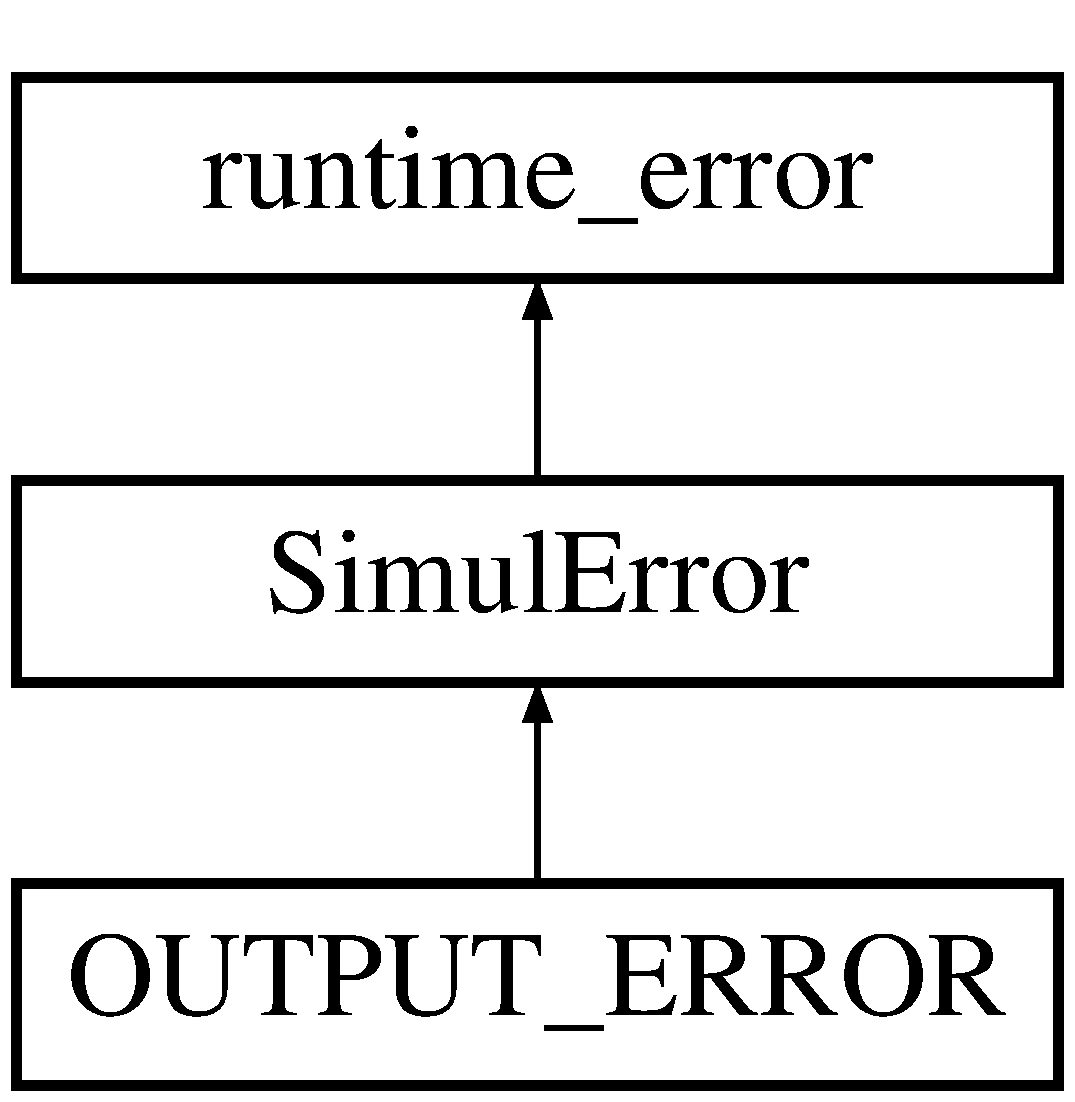
\includegraphics[height=3.000000cm]{classOUTPUT__ERROR}
\end{center}
\end{figure}
\subsection*{Public Member Functions}
\begin{DoxyCompactItemize}
\item 
\hyperlink{classOUTPUT__ERROR_ab3c3ae05be45d2b0ee3f362b61584bef}{O\+U\+T\+P\+U\+T\+\_\+\+E\+R\+R\+OR} (const char $\ast$c)
\item 
\hyperlink{classOUTPUT__ERROR_abdf8edc6e3ea161cc5fac3bf6baffae1}{O\+U\+T\+P\+U\+T\+\_\+\+E\+R\+R\+OR} (const std\+::string \&s)
\end{DoxyCompactItemize}
\subsection*{Additional Inherited Members}


\subsection{Constructor \& Destructor Documentation}
\mbox{\Hypertarget{classOUTPUT__ERROR_ab3c3ae05be45d2b0ee3f362b61584bef}\label{classOUTPUT__ERROR_ab3c3ae05be45d2b0ee3f362b61584bef}} 
\index{O\+U\+T\+P\+U\+T\+\_\+\+E\+R\+R\+OR@{O\+U\+T\+P\+U\+T\+\_\+\+E\+R\+R\+OR}!O\+U\+T\+P\+U\+T\+\_\+\+E\+R\+R\+OR@{O\+U\+T\+P\+U\+T\+\_\+\+E\+R\+R\+OR}}
\index{O\+U\+T\+P\+U\+T\+\_\+\+E\+R\+R\+OR@{O\+U\+T\+P\+U\+T\+\_\+\+E\+R\+R\+OR}!O\+U\+T\+P\+U\+T\+\_\+\+E\+R\+R\+OR@{O\+U\+T\+P\+U\+T\+\_\+\+E\+R\+R\+OR}}
\subsubsection{\texorpdfstring{O\+U\+T\+P\+U\+T\+\_\+\+E\+R\+R\+O\+R()}{OUTPUT\_ERROR()}\hspace{0.1cm}{\footnotesize\ttfamily [1/2]}}
{\footnotesize\ttfamily O\+U\+T\+P\+U\+T\+\_\+\+E\+R\+R\+O\+R\+::\+O\+U\+T\+P\+U\+T\+\_\+\+E\+R\+R\+OR (\begin{DoxyParamCaption}\item[{const char $\ast$}]{c }\end{DoxyParamCaption})\hspace{0.3cm}{\ttfamily [inline]}}


\begin{DoxyCode}
63 :0.4,CH:0.35\textcolor{stringliteral}{'. If total is less than 1, it will be completed with RS neurons"}
\end{DoxyCode}
\mbox{\Hypertarget{classOUTPUT__ERROR_abdf8edc6e3ea161cc5fac3bf6baffae1}\label{classOUTPUT__ERROR_abdf8edc6e3ea161cc5fac3bf6baffae1}} 
\index{O\+U\+T\+P\+U\+T\+\_\+\+E\+R\+R\+OR@{O\+U\+T\+P\+U\+T\+\_\+\+E\+R\+R\+OR}!O\+U\+T\+P\+U\+T\+\_\+\+E\+R\+R\+OR@{O\+U\+T\+P\+U\+T\+\_\+\+E\+R\+R\+OR}}
\index{O\+U\+T\+P\+U\+T\+\_\+\+E\+R\+R\+OR@{O\+U\+T\+P\+U\+T\+\_\+\+E\+R\+R\+OR}!O\+U\+T\+P\+U\+T\+\_\+\+E\+R\+R\+OR@{O\+U\+T\+P\+U\+T\+\_\+\+E\+R\+R\+OR}}
\subsubsection{\texorpdfstring{O\+U\+T\+P\+U\+T\+\_\+\+E\+R\+R\+O\+R()}{OUTPUT\_ERROR()}\hspace{0.1cm}{\footnotesize\ttfamily [2/2]}}
{\footnotesize\ttfamily O\+U\+T\+P\+U\+T\+\_\+\+E\+R\+R\+O\+R\+::\+O\+U\+T\+P\+U\+T\+\_\+\+E\+R\+R\+OR (\begin{DoxyParamCaption}\item[{const std\+::string \&}]{s }\end{DoxyParamCaption})\hspace{0.3cm}{\ttfamily [inline]}}


\begin{DoxyCode}
63 :0.4,CH:0.35\textcolor{stringliteral}{'. If total is less than 1, it will be completed with RS neurons"}
\end{DoxyCode}


The documentation for this class was generated from the following file\+:\begin{DoxyCompactItemize}
\item 
/home/celio/myfiles/\+Programmation/semaine5/\+Neuron\+Net/src/\hyperlink{globals_8h}{globals.\+h}\end{DoxyCompactItemize}

\hypertarget{classRandomNumbers}{}\section{Random\+Numbers Class Reference}
\label{classRandomNumbers}\index{Random\+Numbers@{Random\+Numbers}}


{\ttfamily \#include $<$random.\+h$>$}

\subsection*{Public Member Functions}
\begin{Indent}\textbf{ Initializing}\par
{\em The generator \hyperlink{classRandomNumbers_a15ceee85d6d00de12ae76c90aaec2f14}{rng} is a Mersenne twister {\itshape mt19937} engine.

A seed {\itshape s$>$0} can be provided, by default it is seeded with a {\itshape random\+\_\+device}. }\begin{DoxyCompactItemize}
\item 
\hyperlink{classRandomNumbers_aeceac66b253ad00f58e7b2252f18f609}{Random\+Numbers} (unsigned long int s=0)
\end{DoxyCompactItemize}
\end{Indent}
\begin{Indent}\textbf{ Distributions}\par
{\em These functions either return a single number or fill a given vector with random numbers distributed according the specified distributions.

The additional parameters are the standard parameters of these distributions. }\begin{DoxyCompactItemize}
\item 
void \hyperlink{classRandomNumbers_ae226c129494f9055ac37ed1af943d010}{uniform\+\_\+double} (std\+::vector$<$ double $>$ \&, double lower=0, double upper=1)
\item 
double \hyperlink{classRandomNumbers_a1e66bf9926ad3916f3804dd20ea393f1}{uniform\+\_\+double} (double lower=0, double upper=1)
\item 
void \hyperlink{classRandomNumbers_a4ef5917200da65aa267735d389bdf995}{normal} (std\+::vector$<$ double $>$ \&, double mean=0, double sd=1)
\item 
double \hyperlink{classRandomNumbers_abbfcbae72e7dbd048567dd5b8e2ce9d2}{normal} (double mean=0, double sd=1)
\item 
void \hyperlink{classRandomNumbers_a1195251686ad00cd782c9a91a44d983b}{poisson} (std\+::vector$<$ int $>$ \&vect, double mean=1)
\item 
int \hyperlink{classRandomNumbers_ac5bd95dddabde62a74a0d871a66ce2f0}{poisson} (double mean=1)
\end{DoxyCompactItemize}
\end{Indent}
\begin{Indent}\textbf{ Auxiliary function}\par
{\em This takes a vector of indices and re-\/orders it randomly. }\begin{DoxyCompactItemize}
\item 
void \hyperlink{classRandomNumbers_a851aaa7e46922dc22ce984b21b474a4e}{shuffle} (std\+::vector$<$ size\+\_\+t $>$ \&\+\_\+v)
\end{DoxyCompactItemize}
\end{Indent}
\subsection*{Private Attributes}
\begin{DoxyCompactItemize}
\item 
std\+::mt19937 \hyperlink{classRandomNumbers_a15ceee85d6d00de12ae76c90aaec2f14}{rng}
\item 
long int \hyperlink{classRandomNumbers_a83c563bc5ca60f2e5c149244b327d948}{seed}
\end{DoxyCompactItemize}


\subsection{Detailed Description}
This is a random number class based on standard c++-\/11 generators.

This headers declares the global variable \hyperlink{main_8cpp}{\+\_\+\+R\+NG}, a pointer to the unique instance of this class. 

\subsection{Constructor \& Destructor Documentation}
\mbox{\Hypertarget{classRandomNumbers_aeceac66b253ad00f58e7b2252f18f609}\label{classRandomNumbers_aeceac66b253ad00f58e7b2252f18f609}} 
\index{Random\+Numbers@{Random\+Numbers}!Random\+Numbers@{Random\+Numbers}}
\index{Random\+Numbers@{Random\+Numbers}!Random\+Numbers@{Random\+Numbers}}
\subsubsection{\texorpdfstring{Random\+Numbers()}{RandomNumbers()}}
{\footnotesize\ttfamily Random\+Numbers\+::\+Random\+Numbers (\begin{DoxyParamCaption}\item[{unsigned long int}]{s = {\ttfamily 0} }\end{DoxyParamCaption})}


\begin{DoxyCode}
5 \{
6     \textcolor{keywordflow}{if}(s<=0) \{
7         std::random\_device rd;
8         \hyperlink{classRandomNumbers_a83c563bc5ca60f2e5c149244b327d948}{seed} = rd();
9         \}
10     \textcolor{keywordflow}{else} \hyperlink{classRandomNumbers_a83c563bc5ca60f2e5c149244b327d948}{seed} = s;
11         
12     \hyperlink{classRandomNumbers_a15ceee85d6d00de12ae76c90aaec2f14}{rng} = std::mt19937(\hyperlink{classRandomNumbers_a83c563bc5ca60f2e5c149244b327d948}{seed});
13 \}
\end{DoxyCode}


\subsection{Member Function Documentation}
\mbox{\Hypertarget{classRandomNumbers_a4ef5917200da65aa267735d389bdf995}\label{classRandomNumbers_a4ef5917200da65aa267735d389bdf995}} 
\index{Random\+Numbers@{Random\+Numbers}!normal@{normal}}
\index{normal@{normal}!Random\+Numbers@{Random\+Numbers}}
\subsubsection{\texorpdfstring{normal()}{normal()}\hspace{0.1cm}{\footnotesize\ttfamily [1/2]}}
{\footnotesize\ttfamily void Random\+Numbers\+::normal (\begin{DoxyParamCaption}\item[{std\+::vector$<$ double $>$ \&}]{vect,  }\item[{double}]{mean = {\ttfamily 0},  }\item[{double}]{sd = {\ttfamily 1} }\end{DoxyParamCaption})}


\begin{DoxyCode}
30 \{
31     \textcolor{keywordflow}{for} (\textcolor{keyword}{auto}& element : vect) \{
32         element = \hyperlink{classRandomNumbers_a4ef5917200da65aa267735d389bdf995}{normal}(mean, sd);
33     \}
34 \}
\end{DoxyCode}
\mbox{\Hypertarget{classRandomNumbers_abbfcbae72e7dbd048567dd5b8e2ce9d2}\label{classRandomNumbers_abbfcbae72e7dbd048567dd5b8e2ce9d2}} 
\index{Random\+Numbers@{Random\+Numbers}!normal@{normal}}
\index{normal@{normal}!Random\+Numbers@{Random\+Numbers}}
\subsubsection{\texorpdfstring{normal()}{normal()}\hspace{0.1cm}{\footnotesize\ttfamily [2/2]}}
{\footnotesize\ttfamily double Random\+Numbers\+::normal (\begin{DoxyParamCaption}\item[{double}]{mean = {\ttfamily 0},  }\item[{double}]{sd = {\ttfamily 1} }\end{DoxyParamCaption})}


\begin{DoxyCode}
37 \{
38     std::normal\_distribution<> norm(mean, sd);
39     \textcolor{keywordflow}{return} norm(\hyperlink{classRandomNumbers_a15ceee85d6d00de12ae76c90aaec2f14}{rng});
40 \}
\end{DoxyCode}
\mbox{\Hypertarget{classRandomNumbers_a1195251686ad00cd782c9a91a44d983b}\label{classRandomNumbers_a1195251686ad00cd782c9a91a44d983b}} 
\index{Random\+Numbers@{Random\+Numbers}!poisson@{poisson}}
\index{poisson@{poisson}!Random\+Numbers@{Random\+Numbers}}
\subsubsection{\texorpdfstring{poisson()}{poisson()}\hspace{0.1cm}{\footnotesize\ttfamily [1/2]}}
{\footnotesize\ttfamily void Random\+Numbers\+::poisson (\begin{DoxyParamCaption}\item[{std\+::vector$<$ int $>$ \&}]{vect,  }\item[{double}]{mean = {\ttfamily 1} }\end{DoxyParamCaption})}


\begin{DoxyCode}
43 \{
44     \textcolor{keywordflow}{for} (\textcolor{keyword}{auto}& element : vect) \{
45         element = \hyperlink{classRandomNumbers_a1195251686ad00cd782c9a91a44d983b}{poisson}(mean);
46     \}       
47 \}
\end{DoxyCode}
\mbox{\Hypertarget{classRandomNumbers_ac5bd95dddabde62a74a0d871a66ce2f0}\label{classRandomNumbers_ac5bd95dddabde62a74a0d871a66ce2f0}} 
\index{Random\+Numbers@{Random\+Numbers}!poisson@{poisson}}
\index{poisson@{poisson}!Random\+Numbers@{Random\+Numbers}}
\subsubsection{\texorpdfstring{poisson()}{poisson()}\hspace{0.1cm}{\footnotesize\ttfamily [2/2]}}
{\footnotesize\ttfamily int Random\+Numbers\+::poisson (\begin{DoxyParamCaption}\item[{double}]{mean = {\ttfamily 1} }\end{DoxyParamCaption})}


\begin{DoxyCode}
50 \{
51     std::poisson\_distribution<int> pois(mean);
52     \textcolor{keywordflow}{return} pois(\hyperlink{classRandomNumbers_a15ceee85d6d00de12ae76c90aaec2f14}{rng});
53 \}
\end{DoxyCode}
\mbox{\Hypertarget{classRandomNumbers_a851aaa7e46922dc22ce984b21b474a4e}\label{classRandomNumbers_a851aaa7e46922dc22ce984b21b474a4e}} 
\index{Random\+Numbers@{Random\+Numbers}!shuffle@{shuffle}}
\index{shuffle@{shuffle}!Random\+Numbers@{Random\+Numbers}}
\subsubsection{\texorpdfstring{shuffle()}{shuffle()}}
{\footnotesize\ttfamily void Random\+Numbers\+::shuffle (\begin{DoxyParamCaption}\item[{std\+::vector$<$ size\+\_\+t $>$ \&}]{\+\_\+v }\end{DoxyParamCaption})\hspace{0.3cm}{\ttfamily [inline]}}


\begin{DoxyCode}
42 \{std::shuffle(\_v.begin(), \_v.end(), \hyperlink{classRandomNumbers_a15ceee85d6d00de12ae76c90aaec2f14}{rng});\}
\end{DoxyCode}
\mbox{\Hypertarget{classRandomNumbers_ae226c129494f9055ac37ed1af943d010}\label{classRandomNumbers_ae226c129494f9055ac37ed1af943d010}} 
\index{Random\+Numbers@{Random\+Numbers}!uniform\+\_\+double@{uniform\+\_\+double}}
\index{uniform\+\_\+double@{uniform\+\_\+double}!Random\+Numbers@{Random\+Numbers}}
\subsubsection{\texorpdfstring{uniform\+\_\+double()}{uniform\_double()}\hspace{0.1cm}{\footnotesize\ttfamily [1/2]}}
{\footnotesize\ttfamily void Random\+Numbers\+::uniform\+\_\+double (\begin{DoxyParamCaption}\item[{std\+::vector$<$ double $>$ \&}]{vect,  }\item[{double}]{lower = {\ttfamily 0},  }\item[{double}]{upper = {\ttfamily 1} }\end{DoxyParamCaption})}


\begin{DoxyCode}
16 \{
17     \textcolor{keywordflow}{for} (\textcolor{keyword}{auto}& element : vect) \{
18         element = \hyperlink{classRandomNumbers_ae226c129494f9055ac37ed1af943d010}{uniform\_double}(lower, upper);
19     \}
20 \}
\end{DoxyCode}
\mbox{\Hypertarget{classRandomNumbers_a1e66bf9926ad3916f3804dd20ea393f1}\label{classRandomNumbers_a1e66bf9926ad3916f3804dd20ea393f1}} 
\index{Random\+Numbers@{Random\+Numbers}!uniform\+\_\+double@{uniform\+\_\+double}}
\index{uniform\+\_\+double@{uniform\+\_\+double}!Random\+Numbers@{Random\+Numbers}}
\subsubsection{\texorpdfstring{uniform\+\_\+double()}{uniform\_double()}\hspace{0.1cm}{\footnotesize\ttfamily [2/2]}}
{\footnotesize\ttfamily double Random\+Numbers\+::uniform\+\_\+double (\begin{DoxyParamCaption}\item[{double}]{lower = {\ttfamily 0},  }\item[{double}]{upper = {\ttfamily 1} }\end{DoxyParamCaption})}


\begin{DoxyCode}
24 \{
25     std::uniform\_real\_distribution<double> unif(lower, upper);
26     \textcolor{keywordflow}{return} unif(\hyperlink{classRandomNumbers_a15ceee85d6d00de12ae76c90aaec2f14}{rng});
27 \}
\end{DoxyCode}


\subsection{Member Data Documentation}
\mbox{\Hypertarget{classRandomNumbers_a15ceee85d6d00de12ae76c90aaec2f14}\label{classRandomNumbers_a15ceee85d6d00de12ae76c90aaec2f14}} 
\index{Random\+Numbers@{Random\+Numbers}!rng@{rng}}
\index{rng@{rng}!Random\+Numbers@{Random\+Numbers}}
\subsubsection{\texorpdfstring{rng}{rng}}
{\footnotesize\ttfamily std\+::mt19937 Random\+Numbers\+::rng\hspace{0.3cm}{\ttfamily [private]}}

\mbox{\Hypertarget{classRandomNumbers_a83c563bc5ca60f2e5c149244b327d948}\label{classRandomNumbers_a83c563bc5ca60f2e5c149244b327d948}} 
\index{Random\+Numbers@{Random\+Numbers}!seed@{seed}}
\index{seed@{seed}!Random\+Numbers@{Random\+Numbers}}
\subsubsection{\texorpdfstring{seed}{seed}}
{\footnotesize\ttfamily long int Random\+Numbers\+::seed\hspace{0.3cm}{\ttfamily [private]}}



The documentation for this class was generated from the following files\+:\begin{DoxyCompactItemize}
\item 
/home/celio/myfiles/\+Programmation/semaine5/\+Neuron\+Net/src/\hyperlink{random_8h}{random.\+h}\item 
/home/celio/myfiles/\+Programmation/semaine5/\+Neuron\+Net/src/\hyperlink{random_8cpp}{random.\+cpp}\end{DoxyCompactItemize}

\hypertarget{classSimulation}{}\section{Simulation Class Reference}
\label{classSimulation}\index{Simulation@{Simulation}}


{\ttfamily \#include $<$simulation.\+h$>$}

\subsection*{Classes}
\begin{DoxyCompactItemize}
\item 
struct \hyperlink{structSimulation_1_1intervalConstr}{interval\+Constr}
\end{DoxyCompactItemize}
\subsection*{Public Member Functions}
\begin{DoxyCompactItemize}
\item 
\hyperlink{classSimulation_a26f2ed7943035d802b1b2182ba04af12}{Simulation} (const int \+\_\+s, const int \+\_\+t, const double \+\_\+i=0.\+2)
\item 
\hyperlink{classSimulation_a2cc0f2dc7164778a64462d8b9ec5206d}{Simulation} (int, char $\ast$$\ast$)
\item 
void \hyperlink{classSimulation_acd6ce915b07465d9aaaa5fdcbb5ae077}{load\+\_\+configuration} (const std\+::string \&infile)
\item 
void \hyperlink{classSimulation_afc095e76c2bcee6d31a4614022d609c3}{parse\+\_\+types} (std\+::string)
\item 
size\+\_\+t \hyperlink{classSimulation_a7d0ca858dfec187001ecbab2081f9d04}{size\+\_\+type} (const std\+::string \&\+\_\+s) const
\item 
void \hyperlink{classSimulation_ae5c367f87c0b5dc9740bc6d00e44e72c}{run} ()
\end{DoxyCompactItemize}
\subsection*{Private Member Functions}
\begin{DoxyCompactItemize}
\item 
void \hyperlink{classSimulation_a8f71691f59f56fcb86fa49281c2841db}{parse} (int, char $\ast$$\ast$)
\end{DoxyCompactItemize}
\subsection*{Private Attributes}
\begin{DoxyCompactItemize}
\item 
\hyperlink{classNetwork}{Network} \hyperlink{classSimulation_a980a224fe68945549f217067ffc74f7c}{net}
\item 
int \hyperlink{classSimulation_ae57735a4ad942d9d217fb2235a644d1b}{endtime}
\item 
size\+\_\+t \hyperlink{classSimulation_ae198f9ac020ed6bc6ebbd608ab3f959d}{size}
\item 
double \hyperlink{classSimulation_ad0197878662d63d3ad1699aa7ffe01b2}{degree}
\item 
double \hyperlink{classSimulation_a7fca2f5f79a662f91736b0e5f30598c1}{thalam}
\item 
double \hyperlink{classSimulation_adfda098679d8fcb864ecd87409087d02}{streng}
\item 
double \hyperlink{classSimulation_a14c04fb020df35f875b1f5b2aab7a562}{inhib}
\item 
std\+::string \hyperlink{classSimulation_a9ad4c807c6ddf9066041f764f0ccb9dc}{output}
\item 
std\+::map$<$ std\+::string, size\+\_\+t $>$ \hyperlink{classSimulation_a445d67187d6cc08c4c098ca498ee87d7}{ntypes}
\end{DoxyCompactItemize}


\subsection{Detailed Description}
This is the main class. It manages user inputs, defines the simulation parameters and constructs the \hyperlink{classNetwork}{Network} \hyperlink{classSimulation_a980a224fe68945549f217067ffc74f7c}{net}. It then runs the simulation and prints the results to the output streams. These streams can be files with names based on the string \hyperlink{classSimulation_a9ad4c807c6ddf9066041f764f0ccb9dc}{output} with a suffix.

\hyperlink{classSimulation}{Simulation} parameters\+:
\begin{DoxyItemize}
\item \hyperlink{classSimulation_ae57735a4ad942d9d217fb2235a644d1b}{endtime} \+: total number of time-\/steps, (durée de la simulation)
\item \hyperlink{classSimulation_ae198f9ac020ed6bc6ebbd608ab3f959d}{size} \+: total number of neurons, (nombres de neurones)
\item \hyperlink{classSimulation_ad0197878662d63d3ad1699aa7ffe01b2}{degree} \+: average connectivity of a neuron, (connectivité moyenne -\/$>$ λ)
\item \hyperlink{classSimulation_a7fca2f5f79a662f91736b0e5f30598c1}{thalam} \+: st. dev. of thalamic input (for excitatory neurons),
\item \hyperlink{classSimulation_adfda098679d8fcb864ecd87409087d02}{streng} \+: average intensity of connections, (intensité moyenne des connections)
\item \hyperlink{classSimulation_a14c04fb020df35f875b1f5b2aab7a562}{inhib} \+: fraction of inhibitory neurons in the network, (proportion de neurons excitateurs)
\end{DoxyItemize}

The map \hyperlink{classSimulation_a445d67187d6cc08c4c098ca498ee87d7}{ntypes} describes the neuron population\+: its keys are the neuron types from \hyperlink{classNeuron_ab4b47274e756b72923d2f8a9a5037d23}{Neuron\+::\+Neuron\+Types} and values are the corresponding counts. 

\subsection{Constructor \& Destructor Documentation}
\mbox{\Hypertarget{classSimulation_a26f2ed7943035d802b1b2182ba04af12}\label{classSimulation_a26f2ed7943035d802b1b2182ba04af12}} 
\index{Simulation@{Simulation}!Simulation@{Simulation}}
\index{Simulation@{Simulation}!Simulation@{Simulation}}
\subsubsection{\texorpdfstring{Simulation()}{Simulation()}\hspace{0.1cm}{\footnotesize\ttfamily [1/2]}}
{\footnotesize\ttfamily Simulation\+::\+Simulation (\begin{DoxyParamCaption}\item[{const int}]{\+\_\+s,  }\item[{const int}]{\+\_\+t,  }\item[{const double}]{\+\_\+i = {\ttfamily 0.2} }\end{DoxyParamCaption})\hspace{0.3cm}{\ttfamily [inline]}}

Default constructor initializes the following variables\+: 
\begin{DoxyParams}{Parameters}
{\em \+\_\+s} & (int)\+: size of network (number of neurons) \\
\hline
{\em \+\_\+t} & (int)\+: duration of simulation (number of time-\/steps) \\
\hline
{\em \+\_\+i} & (double)\+: fraction of inhibitory neurons in the network \\
\hline
\end{DoxyParams}

\begin{DoxyCode}
32         : \hyperlink{classSimulation_ae57735a4ad942d9d217fb2235a644d1b}{endtime}(\_t), \hyperlink{classSimulation_ae198f9ac020ed6bc6ebbd608ab3f959d}{size}(\_s), \hyperlink{classSimulation_ad0197878662d63d3ad1699aa7ffe01b2}{degree}(\hyperlink{globals_8h_a3c5c899006fad97c90bca66b048c0d70}{\_DEGREE\_}), 
      \hyperlink{classSimulation_a7fca2f5f79a662f91736b0e5f30598c1}{thalam}(\hyperlink{globals_8h_a4b57d5977068ad6d3ba5e97802c57410}{\_THALAM\_}), \hyperlink{classSimulation_adfda098679d8fcb864ecd87409087d02}{streng}(\hyperlink{globals_8h_ab582a09d695a9c431d8a1c7a0542c086}{\_STRENG\_}), \hyperlink{classSimulation_a14c04fb020df35f875b1f5b2aab7a562}{inhib}(\_i) \{\}
\end{DoxyCode}
\mbox{\Hypertarget{classSimulation_a2cc0f2dc7164778a64462d8b9ec5206d}\label{classSimulation_a2cc0f2dc7164778a64462d8b9ec5206d}} 
\index{Simulation@{Simulation}!Simulation@{Simulation}}
\index{Simulation@{Simulation}!Simulation@{Simulation}}
\subsubsection{\texorpdfstring{Simulation()}{Simulation()}\hspace{0.1cm}{\footnotesize\ttfamily [2/2]}}
{\footnotesize\ttfamily Simulation\+::\+Simulation (\begin{DoxyParamCaption}\item[{int}]{argc,  }\item[{char $\ast$$\ast$}]{argv }\end{DoxyParamCaption})}

Constructor based on user inputs, takes command-\/line arguments and passes them to \hyperlink{classSimulation_a8f71691f59f56fcb86fa49281c2841db}{parse}. 
\begin{DoxyCode}
5                                             \{
6     \hyperlink{classSimulation_a8f71691f59f56fcb86fa49281c2841db}{parse}(argc, argv);
7 \}
\end{DoxyCode}


\subsection{Member Function Documentation}
\mbox{\Hypertarget{classSimulation_acd6ce915b07465d9aaaa5fdcbb5ae077}\label{classSimulation_acd6ce915b07465d9aaaa5fdcbb5ae077}} 
\index{Simulation@{Simulation}!load\+\_\+configuration@{load\+\_\+configuration}}
\index{load\+\_\+configuration@{load\+\_\+configuration}!Simulation@{Simulation}}
\subsubsection{\texorpdfstring{load\+\_\+configuration()}{load\_configuration()}}
{\footnotesize\ttfamily void Simulation\+::load\+\_\+configuration (\begin{DoxyParamCaption}\item[{const std\+::string \&}]{infile }\end{DoxyParamCaption})}

Construct a network as specified in a configuration file 
\begin{DoxyParams}{Parameters}
{\em infile} & (string)\+: filename \\
\hline
\end{DoxyParams}

\begin{DoxyCode}
82                                                            \{
83     \hyperlink{classSimulation_a445d67187d6cc08c4c098ca498ee87d7}{ntypes}.clear();
84     std::vector<NeuronParams> neurons;
85     std::vector<std::string> neurtyp;
86     std::map<size\_t, size\_t> indexmap;
87     \hyperlink{network_8h_a889f48bcec09c9d72a03648e911c5ff5}{linkmap} linklist;
88     std::vector<double> npoten;
89     \hyperlink{classSimulation_ae198f9ac020ed6bc6ebbd608ab3f959d}{size} = 0;
90     \textcolor{keywordflow}{try} \{
91         std::ifstream confstr(infile);
92         std::string item, key, line;
93         \textcolor{keywordtype}{double} value, poten;
94         \textcolor{keywordtype}{size\_t} nindex;
95         \hyperlink{structNeuronParams}{NeuronParams} nparams;
96         \textcolor{keywordflow}{if} (confstr.is\_open()) \{
97             \textcolor{keywordflow}{while} (std::getline(confstr, line)) \{
98                 \textcolor{comment}{// This removes all spaces from the string}
99                 line.erase(std::remove\_if(line.begin(), line.end(), isspace), line.end());
100                 \textcolor{comment}{// comment lines start with #}
101                 \textcolor{keywordflow}{if} (line[0] == \textcolor{charliteral}{'#'}) \textcolor{keywordflow}{continue};
102                 std::stringstream ss(line);
103                 std::getline(ss, item, \textcolor{charliteral}{';'});
104                 key = item.substr(0, 4);
105                 std::transform(key.begin(), key.end(), key.begin(), ::tolower);
106                 \textcolor{keywordflow}{if} (key.compare(\textcolor{stringliteral}{"link"}) == 0) \{
107                     \textcolor{keywordflow}{while} (std::getline(ss, item, \textcolor{charliteral}{';'})) \{
108                         \textcolor{keywordtype}{size\_t} split = item.find(\textcolor{charliteral}{','}),
109                             split2 = item.find(\textcolor{charliteral}{':'});
110                         \textcolor{keywordtype}{size\_t} from = stoi(item.substr(0, split)), 
111                             to = stoi(item.substr(split+1, split2));
112                         \textcolor{keywordtype}{double} str = stod(item.substr(split2+1));
113                         linklist.insert(\{\{from, to\}, str\});
114                     \}
115                 \} \textcolor{keywordflow}{else} \{
116                     nindex = stoi(item);
117                     std::getline(ss, item, \textcolor{charliteral}{';'});
118                     nparams = \hyperlink{classNeuron_a4e5c4e0a512460dd59449a0bec4d0db7}{Neuron::type\_default}(item);
119                     neurtyp.push\_back(item);
120                     \hyperlink{classSimulation_a445d67187d6cc08c4c098ca498ee87d7}{ntypes}[item]++;
121                     poten = \hyperlink{globals_8h_aeef69e4cb5a7aa8b2dc851c334613c2e}{\_REST\_VAL\_};
122                     \textcolor{keywordflow}{while} (std::getline(ss, item, \textcolor{charliteral}{';'})) \{
123                         \textcolor{keywordtype}{size\_t} split = item.find(\textcolor{charliteral}{'='});
124                         key = item.substr(0, split);
125                         std::transform(key.begin(), key.end(), key.begin(), ::tolower);
126                         value = stod(item.substr(split+1));
127                         \textcolor{keywordflow}{if}      (key[0] == \textcolor{charliteral}{'a'}) nparams.\hyperlink{structNeuronParams_a359703733f5e70bbd67d019e45a3bc85}{a} = value;
128                         \textcolor{keywordflow}{else} \textcolor{keywordflow}{if} (key[0] == \textcolor{charliteral}{'b'}) nparams.\hyperlink{structNeuronParams_abd1bd37179d8efa115a8749f9252f77d}{b} = value;
129                         \textcolor{keywordflow}{else} \textcolor{keywordflow}{if} (key[0] == \textcolor{charliteral}{'c'}) nparams.\hyperlink{structNeuronParams_a5df2ced2526eb84af2c8d2d34d9bfd93}{c} = value;
130                         \textcolor{keywordflow}{else} \textcolor{keywordflow}{if} (key[0] == \textcolor{charliteral}{'d'}) nparams.\hyperlink{structNeuronParams_af2bd3bad3bc5532186cdc8d056a10cfb}{d} = value;
131                         \textcolor{keywordflow}{else} \textcolor{keywordflow}{if} (key[0] == \textcolor{charliteral}{'i'}) nparams.\hyperlink{structNeuronParams_a751856d77a821cbd361b774d8653bbe6}{inhib} = (value>0);
132                         \textcolor{keywordflow}{else} \textcolor{keywordflow}{if} (key[0] == \textcolor{charliteral}{'v'}) poten = value;
133                     \}
134                     indexmap[nindex] = \hyperlink{classSimulation_ae198f9ac020ed6bc6ebbd608ab3f959d}{size};
135                     neurons.push\_back(nparams);
136                     npoten.push\_back(poten);
137                     \hyperlink{classSimulation_ae198f9ac020ed6bc6ebbd608ab3f959d}{size}++;
138                 \}
139             \}
140             confstr.close();
141         \} \textcolor{keywordflow}{else} \textcolor{keywordflow}{throw}(\hyperlink{classCFILE__ERROR}{CFILE\_ERROR}(\textcolor{stringliteral}{"Could not open configuration file "} + infile));
142     \} \textcolor{keywordflow}{catch}(std::ifstream::failure &e) \{
143         \textcolor{keywordflow}{throw}(\hyperlink{classCFILE__ERROR}{CFILE\_ERROR}(\textcolor{stringliteral}{"Error with configuration file "} + infile + \textcolor{stringliteral}{": "} + e.what()));
144     \}
145     \hyperlink{classSimulation_a980a224fe68945549f217067ffc74f7c}{net}.\hyperlink{classNetwork_ad91ae24f308dd2b46ff76396fcdb9765}{resize}(\hyperlink{classSimulation_ae198f9ac020ed6bc6ebbd608ab3f959d}{size}, \hyperlink{classSimulation_a14c04fb020df35f875b1f5b2aab7a562}{inhib});
146     \hyperlink{classSimulation_a980a224fe68945549f217067ffc74f7c}{net}.\hyperlink{classNetwork_a40daf6578a6146f4c339f0efffd5070d}{set\_types\_params}(neurtyp, neurons);
147     \hyperlink{classSimulation_a980a224fe68945549f217067ffc74f7c}{net}.\hyperlink{classNetwork_a699416a6462f2da6a5f6cddb30f31440}{set\_values}(npoten);
148     \textcolor{keywordflow}{if} (linklist.empty()) \hyperlink{classSimulation_a980a224fe68945549f217067ffc74f7c}{net}.\hyperlink{classNetwork_a681d8f731ce258376a20f9bf062b943b}{random\_connect}(\hyperlink{classSimulation_ad0197878662d63d3ad1699aa7ffe01b2}{degree}, 
      \hyperlink{classSimulation_adfda098679d8fcb864ecd87409087d02}{streng});
149     \textcolor{keywordflow}{else} \textcolor{keywordflow}{for} (\textcolor{keyword}{auto} I : linklist) 
150              \hyperlink{classSimulation_a980a224fe68945549f217067ffc74f7c}{net}.\hyperlink{classNetwork_a6ebe0899329973e4924997a25e205856}{add\_link}(indexmap[I.first.first], indexmap[I.first.second], I.second);
151 \}
\end{DoxyCode}
\mbox{\Hypertarget{classSimulation_a8f71691f59f56fcb86fa49281c2841db}\label{classSimulation_a8f71691f59f56fcb86fa49281c2841db}} 
\index{Simulation@{Simulation}!parse@{parse}}
\index{parse@{parse}!Simulation@{Simulation}}
\subsubsection{\texorpdfstring{parse()}{parse()}}
{\footnotesize\ttfamily void Simulation\+::parse (\begin{DoxyParamCaption}\item[{int}]{argc,  }\item[{char $\ast$$\ast$}]{argv }\end{DoxyParamCaption})\hspace{0.3cm}{\ttfamily [private]}}

Uses \href{http://tclap.sourceforge.net/html/index.html}{\tt T\+C\+L\+AP} to parse user inputs. 
\begin{DoxyCode}
9                                             \{
10     intervalConstr allowedProperty;
11     TCLAP::CmdLine cmd(\hyperlink{globals_8h_a956c975dbd329dd2c44bf0707ec87928}{\_PRGRM\_TEXT\_});
12     TCLAP::ValueArg<int> sizeArg(\textcolor{stringliteral}{"N"}, \textcolor{stringliteral}{"number"}, \hyperlink{globals_8h_ad6ed0803f0ba1dad283a5f8d223d0771}{\_SIZE\_TEXT\_}, \textcolor{keyword}{false}, 
      \hyperlink{globals_8h_a9acff32baef7c1401d1e2166b0d999c2}{\_SIZE\_}, \textcolor{stringliteral}{"int"});
13     cmd.add(sizeArg);
14     TCLAP::ValueArg<int> timeArg(\textcolor{stringliteral}{"t"}, \textcolor{stringliteral}{"time"}, \hyperlink{globals_8h_a7fb73d75d8e6fe521bc287693f96dea2}{\_TIME\_TEXT\_},  \textcolor{keyword}{false}, 
      \hyperlink{globals_8h_afd5f7c089a6bddd276552473544f977b}{\_TIME\_}, \textcolor{stringliteral}{"int"});
15     cmd.add(timeArg);
16     TCLAP::ValueArg<double> degreeArg(\textcolor{stringliteral}{"d"}, \textcolor{stringliteral}{"degree"}, \hyperlink{globals_8h_a974f4a347352636e3eff38fc6ed15f4e}{\_DEGREE\_TEXT\_},  \textcolor{keyword}{false}, 
      \hyperlink{globals_8h_a3c5c899006fad97c90bca66b048c0d70}{\_DEGREE\_}, \textcolor{stringliteral}{"double"});
17     cmd.add(degreeArg);
18     TCLAP::ValueArg<double> inhibArg(\textcolor{stringliteral}{"i"}, \textcolor{stringliteral}{"inhibitory"}, \hyperlink{globals_8h_a6bb927b9932f49394eb6d0195160f6f8}{\_INHIB\_TEXT\_},  \textcolor{keyword}{false}, -1, &
      allowedProperty);
19     cmd.add(inhibArg);
20     TCLAP::ValueArg<std::string> typesArg(\textcolor{stringliteral}{"T"}, \textcolor{stringliteral}{"neurontypes"}, \hyperlink{globals_8h_a4ff03ef95ba5d9b77316765cba4510a9}{\_TYPES\_TEXT\_},  \textcolor{keyword}{false}, \textcolor{stringliteral}{""}, \textcolor{stringliteral}{"string
      "});
21     cmd.add(typesArg);
22     TCLAP::ValueArg<std::string> outputArg(\textcolor{stringliteral}{"o"}, \textcolor{stringliteral}{"output"}, \hyperlink{globals_8h_ab48fc9989ecb631747042d17b5cb0057}{\_OUTPUT\_TEXT\_},  \textcolor{keyword}{false}, \textcolor{stringliteral}{""}, \textcolor{stringliteral}{"string"})
      ;
23     cmd.add(outputArg);
24     TCLAP::ValueArg<double> strengthArg(\textcolor{stringliteral}{"s"}, \textcolor{stringliteral}{"strength"}, \hyperlink{globals_8h_a5794ab1a7f457a36aa21f5313bf6d4d9}{\_STRENG\_TEXT\_},  \textcolor{keyword}{false}, 
      \hyperlink{globals_8h_ab582a09d695a9c431d8a1c7a0542c086}{\_STRENG\_}, \textcolor{stringliteral}{"double"});
25     cmd.add(strengthArg);
26     TCLAP::ValueArg<double> thalamArg(\textcolor{stringliteral}{"n"}, \textcolor{stringliteral}{"thalamic"}, \hyperlink{globals_8h_a80eb37fbfc12b802cd576a7c270341a5}{\_THALAM\_TEXT\_},  \textcolor{keyword}{false}, 
      \hyperlink{globals_8h_a4b57d5977068ad6d3ba5e97802c57410}{\_THALAM\_}, \textcolor{stringliteral}{"double"});
27     cmd.add(thalamArg);
28     TCLAP::ValueArg<std::string> cfile(\textcolor{stringliteral}{"c"}, \textcolor{stringliteral}{"config"}, \hyperlink{globals_8h_aba0c47a7a3365cac4542d0d4ffb5d165}{\_CFILE\_TEXT\_}, \textcolor{keyword}{false}, \textcolor{stringliteral}{""}, \textcolor{stringliteral}{"string"});
29     cmd.add(cfile);
30 
31     cmd.parse(argc, argv);
32 
33     \hyperlink{classSimulation_ae57735a4ad942d9d217fb2235a644d1b}{endtime} = timeArg.getValue();
34     \hyperlink{classSimulation_ae198f9ac020ed6bc6ebbd608ab3f959d}{size} = sizeArg.getValue();
35     \hyperlink{classSimulation_ad0197878662d63d3ad1699aa7ffe01b2}{degree} = degreeArg.getValue();
36     \hyperlink{classSimulation_a9ad4c807c6ddf9066041f764f0ccb9dc}{output} = outputArg.getValue();
37     \hyperlink{classSimulation_adfda098679d8fcb864ecd87409087d02}{streng} = strengthArg.getValue();
38     \hyperlink{classSimulation_a7fca2f5f79a662f91736b0e5f30598c1}{thalam} = thalamArg.getValue();
39     \hyperlink{classSimulation_a14c04fb020df35f875b1f5b2aab7a562}{inhib} = inhibArg.getValue();
40     \textcolor{keywordflow}{if} (inhib<=0. || inhib>1.) \hyperlink{classSimulation_a14c04fb020df35f875b1f5b2aab7a562}{inhib} = \hyperlink{globals_8h_a44d0be2c42bc40fe1d6d0006ed762f6d}{\_PROP\_INHIB\_};
41     std::string conf(cfile.getValue()), types(typesArg.getValue());
42     \textcolor{keywordflow}{if} (conf.empty()) \{
43         \hyperlink{classSimulation_a980a224fe68945549f217067ffc74f7c}{net}.\hyperlink{classNetwork_ad91ae24f308dd2b46ff76396fcdb9765}{resize}(\hyperlink{classSimulation_ae198f9ac020ed6bc6ebbd608ab3f959d}{size}, \hyperlink{classSimulation_a14c04fb020df35f875b1f5b2aab7a562}{inhib});
44         \hyperlink{classSimulation_afc095e76c2bcee6d31a4614022d609c3}{parse\_types}(types);
45     \} \textcolor{keywordflow}{else} \hyperlink{classSimulation_acd6ce915b07465d9aaaa5fdcbb5ae077}{load\_configuration}(conf);
46 \}
\end{DoxyCode}
\mbox{\Hypertarget{classSimulation_afc095e76c2bcee6d31a4614022d609c3}\label{classSimulation_afc095e76c2bcee6d31a4614022d609c3}} 
\index{Simulation@{Simulation}!parse\+\_\+types@{parse\+\_\+types}}
\index{parse\+\_\+types@{parse\+\_\+types}!Simulation@{Simulation}}
\subsubsection{\texorpdfstring{parse\+\_\+types()}{parse\_types()}}
{\footnotesize\ttfamily void Simulation\+::parse\+\_\+types (\begin{DoxyParamCaption}\item[{std\+::string}]{types }\end{DoxyParamCaption})}

Parses a string such as {\bfseries FS\+:0.\+2,IB\+:0.\+2,CH\+:0.\+15} and constructs the network accordingly (20\% of {\itshape FS} neurons, 20\% of {\itshape IB} and 15of {\itshape CH}). These neuron types are found in \hyperlink{classNeuron_ab4b47274e756b72923d2f8a9a5037d23}{Neuron\+::\+Neuron\+Types}. The neuron population is completed with default ({\itshape RS}) neurons and randomly connected with \hyperlink{classNetwork_a681d8f731ce258376a20f9bf062b943b}{Network\+::random\+\_\+connect}. 
\begin{DoxyCode}
48                                             \{
49     \hyperlink{classSimulation_a445d67187d6cc08c4c098ca498ee87d7}{ntypes}.clear();
50     \textcolor{keywordflow}{if} (types.empty()) \{
51         \textcolor{keywordtype}{size\_t} nfs(\hyperlink{classSimulation_a14c04fb020df35f875b1f5b2aab7a562}{inhib}*\hyperlink{classSimulation_ae198f9ac020ed6bc6ebbd608ab3f959d}{size}+0.5);
52         \hyperlink{classSimulation_a445d67187d6cc08c4c098ca498ee87d7}{ntypes}[\textcolor{stringliteral}{"FS"}] = nfs;
53     \} \textcolor{keywordflow}{else} \{
54         types.erase(std::remove\_if(types.begin(), types.end(), isspace), types.end());
55         std::string label;
56         std::stringstream ss(types);
57         \textcolor{keywordtype}{size\_t} total = 0;
58         \textcolor{keywordflow}{for} (std::string item; total<\hyperlink{classSimulation_ae198f9ac020ed6bc6ebbd608ab3f959d}{size} && std::getline(ss, item, \textcolor{charliteral}{','}); ) \{
59             \textcolor{keywordtype}{size\_t} split = item.find(\textcolor{charliteral}{':'});
60             label = item.substr(0, split);
61             \textcolor{keywordtype}{double} prop = std::min(std::stod(item.substr(split+1)), 1.0);
62             \textcolor{keywordflow}{if} (prop>0 && label!=\textcolor{stringliteral}{"RS"} && \hyperlink{classNeuron_a3a80c93e7cf5214b5e1a9925742bbe8e}{Neuron::type\_exists}(label)) \{
63                 \textcolor{keywordtype}{size\_t} nums(prop*\hyperlink{classSimulation_ae198f9ac020ed6bc6ebbd608ab3f959d}{size}+0.5);
64                 \textcolor{keywordflow}{if} (total+nums>\hyperlink{classSimulation_ae198f9ac020ed6bc6ebbd608ab3f959d}{size}) nums = \hyperlink{classSimulation_ae198f9ac020ed6bc6ebbd608ab3f959d}{size}-total;
65                 \hyperlink{classSimulation_a445d67187d6cc08c4c098ca498ee87d7}{ntypes}[label] = nums;
66                 total += nums;
67             \}
68         \}
69     \}
70     \hyperlink{classSimulation_a980a224fe68945549f217067ffc74f7c}{net}.\hyperlink{classNetwork_ad1d20020028425cfab199da1942172c9}{set\_default\_params}(\hyperlink{classSimulation_a445d67187d6cc08c4c098ca498ee87d7}{ntypes});
71     \hyperlink{classSimulation_a980a224fe68945549f217067ffc74f7c}{net}.\hyperlink{classNetwork_a681d8f731ce258376a20f9bf062b943b}{random\_connect}(\hyperlink{classSimulation_ad0197878662d63d3ad1699aa7ffe01b2}{degree}, \hyperlink{classSimulation_adfda098679d8fcb864ecd87409087d02}{streng});
72 \}
\end{DoxyCode}
\mbox{\Hypertarget{classSimulation_ae5c367f87c0b5dc9740bc6d00e44e72c}\label{classSimulation_ae5c367f87c0b5dc9740bc6d00e44e72c}} 
\index{Simulation@{Simulation}!run@{run}}
\index{run@{run}!Simulation@{Simulation}}
\subsubsection{\texorpdfstring{run()}{run()}}
{\footnotesize\ttfamily void Simulation\+::run (\begin{DoxyParamCaption}{ }\end{DoxyParamCaption})}

The main operation of this class\+: runs the simulation through a loop with \hyperlink{classSimulation_ae57735a4ad942d9d217fb2235a644d1b}{endtime} steps. Each iteration calls \hyperlink{classNetwork_a4614f267a2238b8a10dfea23b54defac}{Network\+::step} with a random value of thalamic input (\hyperlink{classRandomNumbers_a4ef5917200da65aa267735d389bdf995}{Random\+Numbers\+::normal} distribution), then writes out the results. 
\begin{DoxyCode}
153                      \{
154     std::ofstream outf(\hyperlink{classSimulation_a9ad4c807c6ddf9066041f764f0ccb9dc}{output}), outf2, outf3;
155     \textcolor{keywordflow}{if} (\hyperlink{classSimulation_a9ad4c807c6ddf9066041f764f0ccb9dc}{output}.size() && outf.bad()) 
156         \textcolor{keywordflow}{throw}(\hyperlink{classOUTPUT__ERROR}{OUTPUT\_ERROR}(std::string(\textcolor{stringliteral}{"Cannot write to file "})+
      \hyperlink{classSimulation_a9ad4c807c6ddf9066041f764f0ccb9dc}{output}));
157     std::ostream *\_outf = &std::cout;
158     \textcolor{keywordflow}{if} (outf.is\_open()) \_outf = &outf;
159     \textcolor{keywordflow}{if} (\hyperlink{classSimulation_a9ad4c807c6ddf9066041f764f0ccb9dc}{output}.size()) \{
160         outf2.open(\hyperlink{classSimulation_a9ad4c807c6ddf9066041f764f0ccb9dc}{output}+\textcolor{stringliteral}{"\_traj"});
161         \textcolor{keywordflow}{if} (outf2.bad())
162             \textcolor{keywordflow}{throw}(\hyperlink{classOUTPUT__ERROR}{OUTPUT\_ERROR}(std::string(\textcolor{stringliteral}{"Cannot write to file "})+
      \hyperlink{classSimulation_a9ad4c807c6ddf9066041f764f0ccb9dc}{output}+\textcolor{stringliteral}{"\_traj"}));
163         outf3.open(\hyperlink{classSimulation_a9ad4c807c6ddf9066041f764f0ccb9dc}{output}+\textcolor{stringliteral}{"\_pars"});
164         \textcolor{keywordflow}{if} (outf3.bad())
165             \textcolor{keywordflow}{throw}(\hyperlink{classOUTPUT__ERROR}{OUTPUT\_ERROR}(std::string(\textcolor{stringliteral}{"Cannot write to file "})+
      \hyperlink{classSimulation_a9ad4c807c6ddf9066041f764f0ccb9dc}{output}+\textcolor{stringliteral}{"\_pars"}));
166     \}
167     std::vector<double> thalinput(\hyperlink{classSimulation_ae198f9ac020ed6bc6ebbd608ab3f959d}{size});
168     \hyperlink{classSimulation_a980a224fe68945549f217067ffc74f7c}{net}.\hyperlink{classNetwork_afc43116eb2429aeec0f3c6a54d252142}{print\_params}(&outf3);
169     \textcolor{keywordflow}{if} (outf3.is\_open()) outf3.close();
170     \textcolor{keywordflow}{if} (outf2.is\_open()) \hyperlink{classSimulation_a980a224fe68945549f217067ffc74f7c}{net}.\hyperlink{classNetwork_ab572dd33cb91d9f0aae89c4477809d26}{print\_head}(\hyperlink{classSimulation_a445d67187d6cc08c4c098ca498ee87d7}{ntypes}, &outf2);
171     \textcolor{keywordtype}{int} time = 0;
172     \textcolor{keywordflow}{while} (time<\hyperlink{classSimulation_ae57735a4ad942d9d217fb2235a644d1b}{endtime}) \{
173         \hyperlink{main_8cpp_ad20d7a8b3940b60cfd9cd7188fb503ea}{\_RNG}->\hyperlink{classRandomNumbers_a4ef5917200da65aa267735d389bdf995}{normal}(thalinput, 0, \hyperlink{classSimulation_a7fca2f5f79a662f91736b0e5f30598c1}{thalam});
174         std::set<size\_t> firs = \hyperlink{classSimulation_a980a224fe68945549f217067ffc74f7c}{net}.\hyperlink{classNetwork_a4614f267a2238b8a10dfea23b54defac}{step}(thalinput);
175         time++;
176         (*\_outf) << time;
177         \textcolor{keywordflow}{for} (\textcolor{keywordtype}{size\_t} nn=0; nn<\hyperlink{classSimulation_ae198f9ac020ed6bc6ebbd608ab3f959d}{size}; nn++) (*\_outf) << \textcolor{stringliteral}{" "} << firs.count(nn);
178         (*\_outf) << std::endl;
179         \textcolor{keywordflow}{if} (outf2.is\_open()) \hyperlink{classSimulation_a980a224fe68945549f217067ffc74f7c}{net}.\hyperlink{classNetwork_ae460d31557bba058fdf66e4fe5feb801}{print\_traj}(time, \hyperlink{classSimulation_a445d67187d6cc08c4c098ca498ee87d7}{ntypes}, &outf2);
180     \}
181     \textcolor{keywordflow}{if} (outf2.is\_open()) outf2.close();
182     \textcolor{keywordflow}{if} (outf.is\_open()) outf.close();        
183 \}
\end{DoxyCode}
\mbox{\Hypertarget{classSimulation_a7d0ca858dfec187001ecbab2081f9d04}\label{classSimulation_a7d0ca858dfec187001ecbab2081f9d04}} 
\index{Simulation@{Simulation}!size\+\_\+type@{size\+\_\+type}}
\index{size\+\_\+type@{size\+\_\+type}!Simulation@{Simulation}}
\subsubsection{\texorpdfstring{size\+\_\+type()}{size\_type()}}
{\footnotesize\ttfamily size\+\_\+t Simulation\+::size\+\_\+type (\begin{DoxyParamCaption}\item[{const std\+::string \&}]{\+\_\+s }\end{DoxyParamCaption}) const}

Returns the number of neurons of \hyperlink{classNeuron_ab4b47274e756b72923d2f8a9a5037d23}{type} \+\_\+s. 
\begin{DoxyCode}
74                                                       \{
75     \textcolor{keywordflow}{if} (\hyperlink{classSimulation_a445d67187d6cc08c4c098ca498ee87d7}{ntypes}.count(\_s)) \textcolor{keywordflow}{return} \hyperlink{classSimulation_a445d67187d6cc08c4c098ca498ee87d7}{ntypes}.at(\_s);
76     \textcolor{keywordflow}{if} (\_s != \textcolor{stringliteral}{"RS"})       \textcolor{keywordflow}{return} 0;
77     \textcolor{keywordtype}{size\_t} nrs = \hyperlink{classSimulation_ae198f9ac020ed6bc6ebbd608ab3f959d}{size};
78     \textcolor{keywordflow}{for} (\textcolor{keyword}{auto} I : \hyperlink{classSimulation_a445d67187d6cc08c4c098ca498ee87d7}{ntypes}) nrs -= I.second;
79     \textcolor{keywordflow}{return} nrs;
80 \}
\end{DoxyCode}


\subsection{Member Data Documentation}
\mbox{\Hypertarget{classSimulation_ad0197878662d63d3ad1699aa7ffe01b2}\label{classSimulation_ad0197878662d63d3ad1699aa7ffe01b2}} 
\index{Simulation@{Simulation}!degree@{degree}}
\index{degree@{degree}!Simulation@{Simulation}}
\subsubsection{\texorpdfstring{degree}{degree}}
{\footnotesize\ttfamily double Simulation\+::degree\hspace{0.3cm}{\ttfamily [private]}}

\mbox{\Hypertarget{classSimulation_ae57735a4ad942d9d217fb2235a644d1b}\label{classSimulation_ae57735a4ad942d9d217fb2235a644d1b}} 
\index{Simulation@{Simulation}!endtime@{endtime}}
\index{endtime@{endtime}!Simulation@{Simulation}}
\subsubsection{\texorpdfstring{endtime}{endtime}}
{\footnotesize\ttfamily int Simulation\+::endtime\hspace{0.3cm}{\ttfamily [private]}}

\mbox{\Hypertarget{classSimulation_a14c04fb020df35f875b1f5b2aab7a562}\label{classSimulation_a14c04fb020df35f875b1f5b2aab7a562}} 
\index{Simulation@{Simulation}!inhib@{inhib}}
\index{inhib@{inhib}!Simulation@{Simulation}}
\subsubsection{\texorpdfstring{inhib}{inhib}}
{\footnotesize\ttfamily double Simulation\+::inhib\hspace{0.3cm}{\ttfamily [private]}}

\mbox{\Hypertarget{classSimulation_a980a224fe68945549f217067ffc74f7c}\label{classSimulation_a980a224fe68945549f217067ffc74f7c}} 
\index{Simulation@{Simulation}!net@{net}}
\index{net@{net}!Simulation@{Simulation}}
\subsubsection{\texorpdfstring{net}{net}}
{\footnotesize\ttfamily \hyperlink{classNetwork}{Network} Simulation\+::net\hspace{0.3cm}{\ttfamily [private]}}

\mbox{\Hypertarget{classSimulation_a445d67187d6cc08c4c098ca498ee87d7}\label{classSimulation_a445d67187d6cc08c4c098ca498ee87d7}} 
\index{Simulation@{Simulation}!ntypes@{ntypes}}
\index{ntypes@{ntypes}!Simulation@{Simulation}}
\subsubsection{\texorpdfstring{ntypes}{ntypes}}
{\footnotesize\ttfamily std\+::map$<$ std\+::string, size\+\_\+t $>$ Simulation\+::ntypes\hspace{0.3cm}{\ttfamily [private]}}

\mbox{\Hypertarget{classSimulation_a9ad4c807c6ddf9066041f764f0ccb9dc}\label{classSimulation_a9ad4c807c6ddf9066041f764f0ccb9dc}} 
\index{Simulation@{Simulation}!output@{output}}
\index{output@{output}!Simulation@{Simulation}}
\subsubsection{\texorpdfstring{output}{output}}
{\footnotesize\ttfamily std\+::string Simulation\+::output\hspace{0.3cm}{\ttfamily [private]}}

\mbox{\Hypertarget{classSimulation_ae198f9ac020ed6bc6ebbd608ab3f959d}\label{classSimulation_ae198f9ac020ed6bc6ebbd608ab3f959d}} 
\index{Simulation@{Simulation}!size@{size}}
\index{size@{size}!Simulation@{Simulation}}
\subsubsection{\texorpdfstring{size}{size}}
{\footnotesize\ttfamily size\+\_\+t Simulation\+::size\hspace{0.3cm}{\ttfamily [private]}}

\mbox{\Hypertarget{classSimulation_adfda098679d8fcb864ecd87409087d02}\label{classSimulation_adfda098679d8fcb864ecd87409087d02}} 
\index{Simulation@{Simulation}!streng@{streng}}
\index{streng@{streng}!Simulation@{Simulation}}
\subsubsection{\texorpdfstring{streng}{streng}}
{\footnotesize\ttfamily double Simulation\+::streng\hspace{0.3cm}{\ttfamily [private]}}

\mbox{\Hypertarget{classSimulation_a7fca2f5f79a662f91736b0e5f30598c1}\label{classSimulation_a7fca2f5f79a662f91736b0e5f30598c1}} 
\index{Simulation@{Simulation}!thalam@{thalam}}
\index{thalam@{thalam}!Simulation@{Simulation}}
\subsubsection{\texorpdfstring{thalam}{thalam}}
{\footnotesize\ttfamily double Simulation\+::thalam\hspace{0.3cm}{\ttfamily [private]}}



The documentation for this class was generated from the following files\+:\begin{DoxyCompactItemize}
\item 
/home/celio/myfiles/\+Programmation/semaine5/\+Neuron\+Net/src/\hyperlink{simulation_8h}{simulation.\+h}\item 
/home/celio/myfiles/\+Programmation/semaine5/\+Neuron\+Net/src/\hyperlink{simulation_8cpp}{simulation.\+cpp}\end{DoxyCompactItemize}

\hypertarget{classSimulError}{}\section{Simul\+Error Class Reference}
\label{classSimulError}\index{Simul\+Error@{Simul\+Error}}


{\ttfamily \#include $<$globals.\+h$>$}

Inheritance diagram for Simul\+Error\+:\begin{figure}[H]
\begin{center}
\leavevmode
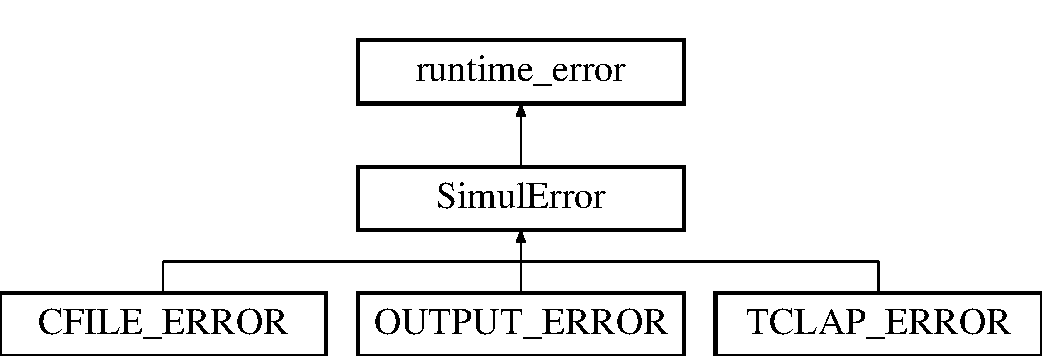
\includegraphics[height=3.000000cm]{classSimulError}
\end{center}
\end{figure}
\subsection*{Public Member Functions}
\begin{DoxyCompactItemize}
\item 
\hyperlink{classSimulError_afaa5c6167e80c55fb3814c1bbcb7dcb9}{Simul\+Error} (const char $\ast$c, int v=0)
\item 
\hyperlink{classSimulError_a475bd5eab2cafd9c6b72471449dc2576}{Simul\+Error} (const std\+::string \&s, int v=0)
\item 
int \hyperlink{classSimulError_a34627c973b586c593d8ed0f7352bc401}{value} () const
\end{DoxyCompactItemize}
\subsection*{Protected Attributes}
\begin{DoxyCompactItemize}
\item 
const int \hyperlink{classSimulError_a5cd98a7eddc7982f5c715ef1c76a1bc2}{code}
\end{DoxyCompactItemize}


\subsection{Constructor \& Destructor Documentation}
\mbox{\Hypertarget{classSimulError_afaa5c6167e80c55fb3814c1bbcb7dcb9}\label{classSimulError_afaa5c6167e80c55fb3814c1bbcb7dcb9}} 
\index{Simul\+Error@{Simul\+Error}!Simul\+Error@{Simul\+Error}}
\index{Simul\+Error@{Simul\+Error}!Simul\+Error@{Simul\+Error}}
\subsubsection{\texorpdfstring{Simul\+Error()}{SimulError()}\hspace{0.1cm}{\footnotesize\ttfamily [1/2]}}
{\footnotesize\ttfamily Simul\+Error\+::\+Simul\+Error (\begin{DoxyParamCaption}\item[{const char $\ast$}]{c,  }\item[{int}]{v = {\ttfamily 0} }\end{DoxyParamCaption})\hspace{0.3cm}{\ttfamily [inline]}}


\begin{DoxyCode}
19 : std::runtime\_error(c), \hyperlink{classSimulError_a5cd98a7eddc7982f5c715ef1c76a1bc2}{code}(v) \{\}
\end{DoxyCode}
\mbox{\Hypertarget{classSimulError_a475bd5eab2cafd9c6b72471449dc2576}\label{classSimulError_a475bd5eab2cafd9c6b72471449dc2576}} 
\index{Simul\+Error@{Simul\+Error}!Simul\+Error@{Simul\+Error}}
\index{Simul\+Error@{Simul\+Error}!Simul\+Error@{Simul\+Error}}
\subsubsection{\texorpdfstring{Simul\+Error()}{SimulError()}\hspace{0.1cm}{\footnotesize\ttfamily [2/2]}}
{\footnotesize\ttfamily Simul\+Error\+::\+Simul\+Error (\begin{DoxyParamCaption}\item[{const std\+::string \&}]{s,  }\item[{int}]{v = {\ttfamily 0} }\end{DoxyParamCaption})\hspace{0.3cm}{\ttfamily [inline]}}


\begin{DoxyCode}
20 : std::runtime\_error(s), \hyperlink{classSimulError_a5cd98a7eddc7982f5c715ef1c76a1bc2}{code}(v) \{\}
\end{DoxyCode}


\subsection{Member Function Documentation}
\mbox{\Hypertarget{classSimulError_a34627c973b586c593d8ed0f7352bc401}\label{classSimulError_a34627c973b586c593d8ed0f7352bc401}} 
\index{Simul\+Error@{Simul\+Error}!value@{value}}
\index{value@{value}!Simul\+Error@{Simul\+Error}}
\subsubsection{\texorpdfstring{value()}{value()}}
{\footnotesize\ttfamily int Simul\+Error\+::value (\begin{DoxyParamCaption}{ }\end{DoxyParamCaption}) const\hspace{0.3cm}{\ttfamily [inline]}}


\begin{DoxyCode}
21 \{\textcolor{keywordflow}{return} \hyperlink{classSimulError_a5cd98a7eddc7982f5c715ef1c76a1bc2}{code};\}
\end{DoxyCode}


\subsection{Member Data Documentation}
\mbox{\Hypertarget{classSimulError_a5cd98a7eddc7982f5c715ef1c76a1bc2}\label{classSimulError_a5cd98a7eddc7982f5c715ef1c76a1bc2}} 
\index{Simul\+Error@{Simul\+Error}!code@{code}}
\index{code@{code}!Simul\+Error@{Simul\+Error}}
\subsubsection{\texorpdfstring{code}{code}}
{\footnotesize\ttfamily const int Simul\+Error\+::code\hspace{0.3cm}{\ttfamily [protected]}}



The documentation for this class was generated from the following file\+:\begin{DoxyCompactItemize}
\item 
/home/celio/myfiles/\+Programmation/semaine5/\+Neuron\+Net/src/\hyperlink{globals_8h}{globals.\+h}\end{DoxyCompactItemize}

\hypertarget{classTCLAP__ERROR}{}\section{T\+C\+L\+A\+P\+\_\+\+E\+R\+R\+OR Class Reference}
\label{classTCLAP__ERROR}\index{T\+C\+L\+A\+P\+\_\+\+E\+R\+R\+OR@{T\+C\+L\+A\+P\+\_\+\+E\+R\+R\+OR}}


{\itshape Specific error codes}  




{\ttfamily \#include $<$globals.\+h$>$}

Inheritance diagram for T\+C\+L\+A\+P\+\_\+\+E\+R\+R\+OR\+:\begin{figure}[H]
\begin{center}
\leavevmode
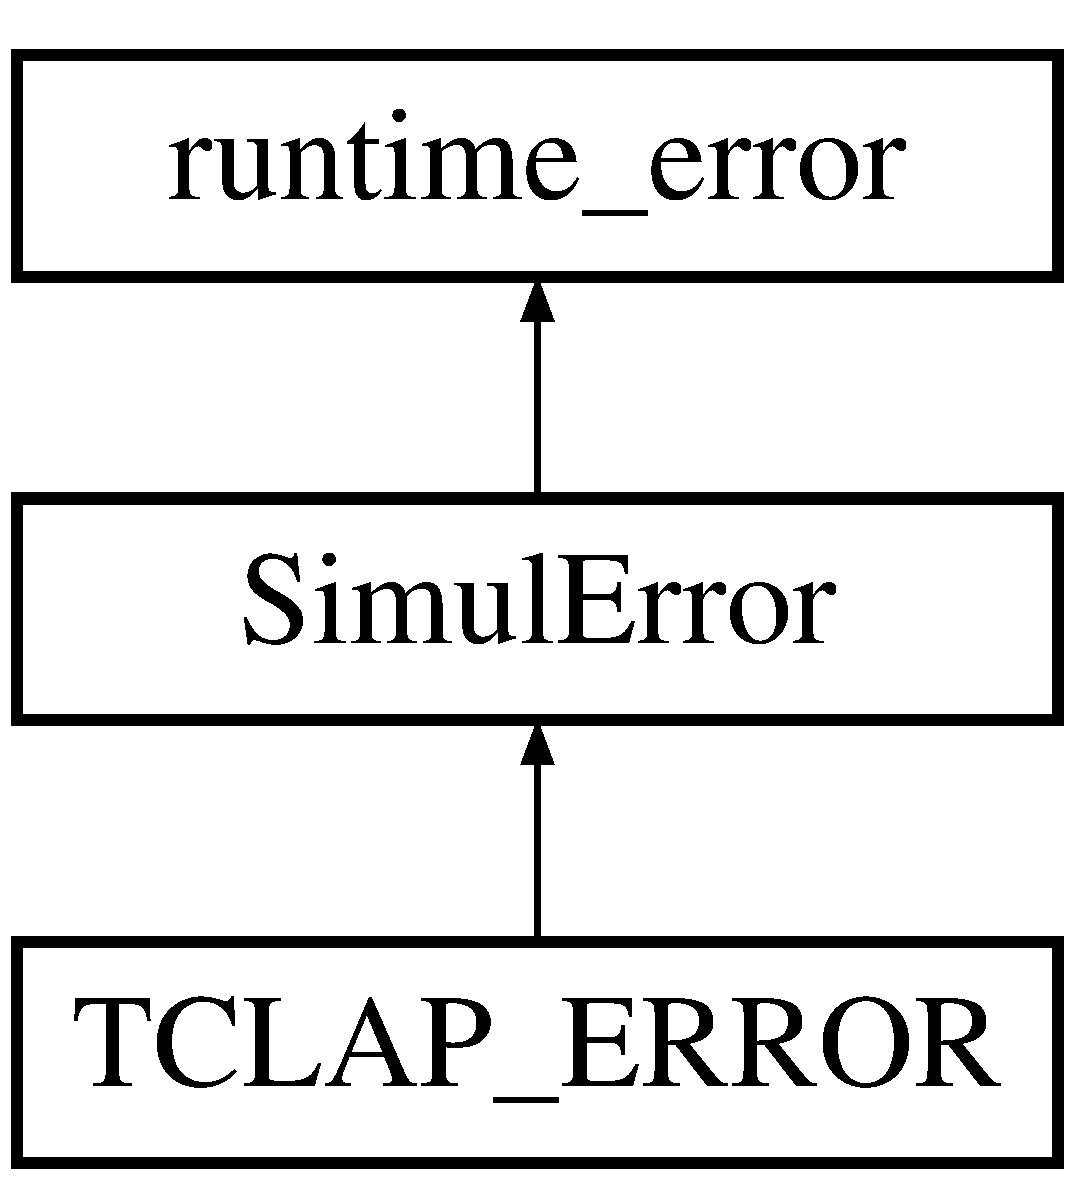
\includegraphics[height=3.000000cm]{classTCLAP__ERROR}
\end{center}
\end{figure}
\subsection*{Public Member Functions}
\begin{DoxyCompactItemize}
\item 
\hyperlink{classTCLAP__ERROR_a9fadfa86a7a882c2db2fc8efcc8cabb4}{T\+C\+L\+A\+P\+\_\+\+E\+R\+R\+OR} (const char $\ast$c)
\item 
\hyperlink{classTCLAP__ERROR_a8df7cf40b000475e793bb76517256db3}{T\+C\+L\+A\+P\+\_\+\+E\+R\+R\+OR} (const std\+::string \&s)
\end{DoxyCompactItemize}
\subsection*{Additional Inherited Members}


\subsection{Detailed Description}
{\itshape Specific error codes} 

\subsection{Constructor \& Destructor Documentation}
\mbox{\Hypertarget{classTCLAP__ERROR_a9fadfa86a7a882c2db2fc8efcc8cabb4}\label{classTCLAP__ERROR_a9fadfa86a7a882c2db2fc8efcc8cabb4}} 
\index{T\+C\+L\+A\+P\+\_\+\+E\+R\+R\+OR@{T\+C\+L\+A\+P\+\_\+\+E\+R\+R\+OR}!T\+C\+L\+A\+P\+\_\+\+E\+R\+R\+OR@{T\+C\+L\+A\+P\+\_\+\+E\+R\+R\+OR}}
\index{T\+C\+L\+A\+P\+\_\+\+E\+R\+R\+OR@{T\+C\+L\+A\+P\+\_\+\+E\+R\+R\+OR}!T\+C\+L\+A\+P\+\_\+\+E\+R\+R\+OR@{T\+C\+L\+A\+P\+\_\+\+E\+R\+R\+OR}}
\subsubsection{\texorpdfstring{T\+C\+L\+A\+P\+\_\+\+E\+R\+R\+O\+R()}{TCLAP\_ERROR()}\hspace{0.1cm}{\footnotesize\ttfamily [1/2]}}
{\footnotesize\ttfamily T\+C\+L\+A\+P\+\_\+\+E\+R\+R\+O\+R\+::\+T\+C\+L\+A\+P\+\_\+\+E\+R\+R\+OR (\begin{DoxyParamCaption}\item[{const char $\ast$}]{c }\end{DoxyParamCaption})\hspace{0.3cm}{\ttfamily [inline]}}


\begin{DoxyCode}
63 :0.4,CH:0.35\textcolor{stringliteral}{'. If total is less than 1, it will be completed with RS neurons"}
\end{DoxyCode}
\mbox{\Hypertarget{classTCLAP__ERROR_a8df7cf40b000475e793bb76517256db3}\label{classTCLAP__ERROR_a8df7cf40b000475e793bb76517256db3}} 
\index{T\+C\+L\+A\+P\+\_\+\+E\+R\+R\+OR@{T\+C\+L\+A\+P\+\_\+\+E\+R\+R\+OR}!T\+C\+L\+A\+P\+\_\+\+E\+R\+R\+OR@{T\+C\+L\+A\+P\+\_\+\+E\+R\+R\+OR}}
\index{T\+C\+L\+A\+P\+\_\+\+E\+R\+R\+OR@{T\+C\+L\+A\+P\+\_\+\+E\+R\+R\+OR}!T\+C\+L\+A\+P\+\_\+\+E\+R\+R\+OR@{T\+C\+L\+A\+P\+\_\+\+E\+R\+R\+OR}}
\subsubsection{\texorpdfstring{T\+C\+L\+A\+P\+\_\+\+E\+R\+R\+O\+R()}{TCLAP\_ERROR()}\hspace{0.1cm}{\footnotesize\ttfamily [2/2]}}
{\footnotesize\ttfamily T\+C\+L\+A\+P\+\_\+\+E\+R\+R\+O\+R\+::\+T\+C\+L\+A\+P\+\_\+\+E\+R\+R\+OR (\begin{DoxyParamCaption}\item[{const std\+::string \&}]{s }\end{DoxyParamCaption})\hspace{0.3cm}{\ttfamily [inline]}}


\begin{DoxyCode}
63 :0.4,CH:0.35\textcolor{stringliteral}{'. If total is less than 1, it will be completed with RS neurons"}
\end{DoxyCode}


The documentation for this class was generated from the following file\+:\begin{DoxyCompactItemize}
\item 
/home/celio/myfiles/\+Programmation/semaine5/\+Neuron\+Net/src/\hyperlink{globals_8h}{globals.\+h}\end{DoxyCompactItemize}

\chapter{File Documentation}
\hypertarget{globals_8h}{}\section{/home/celio/myfiles/\+Programmation/semaine5/\+Neuron\+Net/src/globals.h File Reference}
\label{globals_8h}\index{/home/celio/myfiles/\+Programmation/semaine5/\+Neuron\+Net/src/globals.\+h@{/home/celio/myfiles/\+Programmation/semaine5/\+Neuron\+Net/src/globals.\+h}}
{\ttfamily \#include $<$algorithm$>$}\newline
{\ttfamily \#include $<$stdexcept$>$}\newline
{\ttfamily \#include $<$iostream$>$}\newline
{\ttfamily \#include $<$fstream$>$}\newline
{\ttfamily \#include $<$sstream$>$}\newline
{\ttfamily \#include $<$array$>$}\newline
{\ttfamily \#include $<$set$>$}\newline
{\ttfamily \#include $<$vector$>$}\newline
{\ttfamily \#include $<$map$>$}\newline
{\ttfamily \#include $<$string$>$}\newline
{\ttfamily \#include $<$cmath$>$}\newline
\subsection*{Classes}
\begin{DoxyCompactItemize}
\item 
class \hyperlink{classSimulError}{Simul\+Error}
\item 
class \hyperlink{classTCLAP__ERROR}{T\+C\+L\+A\+P\+\_\+\+E\+R\+R\+OR}
\begin{DoxyCompactList}\small\item\em {\itshape Specific error codes} \end{DoxyCompactList}\item 
class \hyperlink{classOUTPUT__ERROR}{O\+U\+T\+P\+U\+T\+\_\+\+E\+R\+R\+OR}
\item 
class \hyperlink{classCFILE__ERROR}{C\+F\+I\+L\+E\+\_\+\+E\+R\+R\+OR}
\end{DoxyCompactItemize}
\subsection*{Macros}
\begin{DoxyCompactItemize}
\item 
\#define \hyperlink{globals_8h_a9acbb7768cf11ccc612674f266a9182b}{\+\_\+\+S\+I\+M\+U\+L\+E\+R\+R\+\_\+}(\+\_\+N,  \+\_\+id)
\item 
\#define \hyperlink{globals_8h_a9acff32baef7c1401d1e2166b0d999c2}{\+\_\+\+S\+I\+Z\+E\+\_\+}~100
\item 
\#define \hyperlink{globals_8h_afd5f7c089a6bddd276552473544f977b}{\+\_\+\+T\+I\+M\+E\+\_\+}~10
\item 
\#define \hyperlink{globals_8h_a3c5c899006fad97c90bca66b048c0d70}{\+\_\+\+D\+E\+G\+R\+E\+E\+\_\+}~4
\item 
\#define \hyperlink{globals_8h_ab582a09d695a9c431d8a1c7a0542c086}{\+\_\+\+S\+T\+R\+E\+N\+G\+\_\+}~.\+25
\item 
\#define \hyperlink{globals_8h_a4b57d5977068ad6d3ba5e97802c57410}{\+\_\+\+T\+H\+A\+L\+A\+M\+\_\+}~5
\item 
\#define \hyperlink{globals_8h_a44d0be2c42bc40fe1d6d0006ed762f6d}{\+\_\+\+P\+R\+O\+P\+\_\+\+I\+N\+H\+I\+B\+\_\+}~0.\+2
\item 
\#define \hyperlink{globals_8h_a4105fbbc586623b6fcce28eec8417c29}{\+\_\+\+F\+I\+R\+I\+N\+G\+\_\+\+T\+H\+\_\+}~30
\item 
\#define \hyperlink{globals_8h_aeef69e4cb5a7aa8b2dc851c334613c2e}{\+\_\+\+R\+E\+S\+T\+\_\+\+V\+A\+L\+\_\+}~-\/65.\+0
\item 
\#define \hyperlink{globals_8h_a6ed83a2720f26c982b486bcd7398bda4}{\+\_\+\+A\+V\+A\+R\+\_\+}~.\+8
\item 
\#define \hyperlink{globals_8h_afeb27810410b4ad253c0cc446b56cbfd}{\+\_\+\+B\+V\+A\+R\+\_\+}~.\+25
\item 
\#define \hyperlink{globals_8h_a6f19bdc067b5267c5f96db47062fef17}{\+\_\+\+C\+V\+A\+R\+\_\+}~0.\+2307692
\item 
\#define \hyperlink{globals_8h_ab562b7e46b970a109c23f7e3eaa10bf2}{\+\_\+\+D\+V\+A\+R\+\_\+}~.\+75
\item 
\#define \hyperlink{globals_8h_a956c975dbd329dd2c44bf0707ec87928}{\+\_\+\+P\+R\+G\+R\+M\+\_\+\+T\+E\+X\+T\+\_\+}~\char`\"{}Simulation of the Izhikevich neuron model\char`\"{}
\item 
\#define \hyperlink{globals_8h_a7fb73d75d8e6fe521bc287693f96dea2}{\+\_\+\+T\+I\+M\+E\+\_\+\+T\+E\+X\+T\+\_\+}~\char`\"{}Number of time-\/steps\char`\"{}
\item 
\#define \hyperlink{globals_8h_ad6ed0803f0ba1dad283a5f8d223d0771}{\+\_\+\+S\+I\+Z\+E\+\_\+\+T\+E\+X\+T\+\_\+}~\char`\"{}Number of neurons\char`\"{}
\item 
\#define \hyperlink{globals_8h_a974f4a347352636e3eff38fc6ed15f4e}{\+\_\+\+D\+E\+G\+R\+E\+E\+\_\+\+T\+E\+X\+T\+\_\+}~\char`\"{}Average connectivity between neurons\char`\"{}
\item 
\#define \hyperlink{globals_8h_a6bb927b9932f49394eb6d0195160f6f8}{\+\_\+\+I\+N\+H\+I\+B\+\_\+\+T\+E\+X\+T\+\_\+}~\char`\"{}Proportion of inhibitory (FS) neurons, the complement will be RS neurons\char`\"{}
\item 
\#define \hyperlink{globals_8h_a5794ab1a7f457a36aa21f5313bf6d4d9}{\+\_\+\+S\+T\+R\+E\+N\+G\+\_\+\+T\+E\+X\+T\+\_\+}~\char`\"{}Average link strength for excitatory neurons (inhibitory is the double)\char`\"{}
\item 
\#define \hyperlink{globals_8h_a80eb37fbfc12b802cd576a7c270341a5}{\+\_\+\+T\+H\+A\+L\+A\+M\+\_\+\+T\+E\+X\+T\+\_\+}~\char`\"{}Std deviation of thalamic input \hyperlink{test__main_8cpp_aedb3acb007b8cca8efc63eed08f45705}{noise}\char`\"{}
\item 
\#define \hyperlink{globals_8h_a4ff03ef95ba5d9b77316765cba4510a9}{\+\_\+\+T\+Y\+P\+E\+S\+\_\+\+T\+E\+X\+T\+\_\+}~\char`\"{}Proportions of each type of neurons as a list like \textquotesingle{}I\+B\+:0.\+4,C\+H\+:0.\+35\textquotesingle{}. If total is less than 1, it will be completed with RS neurons\char`\"{}
\item 
\#define \hyperlink{globals_8h_ab48fc9989ecb631747042d17b5cb0057}{\+\_\+\+O\+U\+T\+P\+U\+T\+\_\+\+T\+E\+X\+T\+\_\+}~\char`\"{}Output file name (default is output to screen)\char`\"{}
\item 
\#define \hyperlink{globals_8h_aba0c47a7a3365cac4542d0d4ffb5d165}{\+\_\+\+C\+F\+I\+L\+E\+\_\+\+T\+E\+X\+T\+\_\+}~\char`\"{}Configuration file name\char`\"{}
\end{DoxyCompactItemize}


\subsection{Macro Definition Documentation}
\mbox{\Hypertarget{globals_8h_a6ed83a2720f26c982b486bcd7398bda4}\label{globals_8h_a6ed83a2720f26c982b486bcd7398bda4}} 
\index{globals.\+h@{globals.\+h}!\+\_\+\+A\+V\+A\+R\+\_\+@{\+\_\+\+A\+V\+A\+R\+\_\+}}
\index{\+\_\+\+A\+V\+A\+R\+\_\+@{\+\_\+\+A\+V\+A\+R\+\_\+}!globals.\+h@{globals.\+h}}
\subsubsection{\texorpdfstring{\+\_\+\+A\+V\+A\+R\+\_\+}{\_AVAR\_}}
{\footnotesize\ttfamily \#define \+\_\+\+A\+V\+A\+R\+\_\+~.\+8}

\mbox{\Hypertarget{globals_8h_afeb27810410b4ad253c0cc446b56cbfd}\label{globals_8h_afeb27810410b4ad253c0cc446b56cbfd}} 
\index{globals.\+h@{globals.\+h}!\+\_\+\+B\+V\+A\+R\+\_\+@{\+\_\+\+B\+V\+A\+R\+\_\+}}
\index{\+\_\+\+B\+V\+A\+R\+\_\+@{\+\_\+\+B\+V\+A\+R\+\_\+}!globals.\+h@{globals.\+h}}
\subsubsection{\texorpdfstring{\+\_\+\+B\+V\+A\+R\+\_\+}{\_BVAR\_}}
{\footnotesize\ttfamily \#define \+\_\+\+B\+V\+A\+R\+\_\+~.\+25}

\mbox{\Hypertarget{globals_8h_aba0c47a7a3365cac4542d0d4ffb5d165}\label{globals_8h_aba0c47a7a3365cac4542d0d4ffb5d165}} 
\index{globals.\+h@{globals.\+h}!\+\_\+\+C\+F\+I\+L\+E\+\_\+\+T\+E\+X\+T\+\_\+@{\+\_\+\+C\+F\+I\+L\+E\+\_\+\+T\+E\+X\+T\+\_\+}}
\index{\+\_\+\+C\+F\+I\+L\+E\+\_\+\+T\+E\+X\+T\+\_\+@{\+\_\+\+C\+F\+I\+L\+E\+\_\+\+T\+E\+X\+T\+\_\+}!globals.\+h@{globals.\+h}}
\subsubsection{\texorpdfstring{\+\_\+\+C\+F\+I\+L\+E\+\_\+\+T\+E\+X\+T\+\_\+}{\_CFILE\_TEXT\_}}
{\footnotesize\ttfamily \#define \+\_\+\+C\+F\+I\+L\+E\+\_\+\+T\+E\+X\+T\+\_\+~\char`\"{}Configuration file name\char`\"{}}

\mbox{\Hypertarget{globals_8h_a6f19bdc067b5267c5f96db47062fef17}\label{globals_8h_a6f19bdc067b5267c5f96db47062fef17}} 
\index{globals.\+h@{globals.\+h}!\+\_\+\+C\+V\+A\+R\+\_\+@{\+\_\+\+C\+V\+A\+R\+\_\+}}
\index{\+\_\+\+C\+V\+A\+R\+\_\+@{\+\_\+\+C\+V\+A\+R\+\_\+}!globals.\+h@{globals.\+h}}
\subsubsection{\texorpdfstring{\+\_\+\+C\+V\+A\+R\+\_\+}{\_CVAR\_}}
{\footnotesize\ttfamily \#define \+\_\+\+C\+V\+A\+R\+\_\+~0.\+2307692}

\mbox{\Hypertarget{globals_8h_a3c5c899006fad97c90bca66b048c0d70}\label{globals_8h_a3c5c899006fad97c90bca66b048c0d70}} 
\index{globals.\+h@{globals.\+h}!\+\_\+\+D\+E\+G\+R\+E\+E\+\_\+@{\+\_\+\+D\+E\+G\+R\+E\+E\+\_\+}}
\index{\+\_\+\+D\+E\+G\+R\+E\+E\+\_\+@{\+\_\+\+D\+E\+G\+R\+E\+E\+\_\+}!globals.\+h@{globals.\+h}}
\subsubsection{\texorpdfstring{\+\_\+\+D\+E\+G\+R\+E\+E\+\_\+}{\_DEGREE\_}}
{\footnotesize\ttfamily \#define \+\_\+\+D\+E\+G\+R\+E\+E\+\_\+~4}

\mbox{\Hypertarget{globals_8h_a974f4a347352636e3eff38fc6ed15f4e}\label{globals_8h_a974f4a347352636e3eff38fc6ed15f4e}} 
\index{globals.\+h@{globals.\+h}!\+\_\+\+D\+E\+G\+R\+E\+E\+\_\+\+T\+E\+X\+T\+\_\+@{\+\_\+\+D\+E\+G\+R\+E\+E\+\_\+\+T\+E\+X\+T\+\_\+}}
\index{\+\_\+\+D\+E\+G\+R\+E\+E\+\_\+\+T\+E\+X\+T\+\_\+@{\+\_\+\+D\+E\+G\+R\+E\+E\+\_\+\+T\+E\+X\+T\+\_\+}!globals.\+h@{globals.\+h}}
\subsubsection{\texorpdfstring{\+\_\+\+D\+E\+G\+R\+E\+E\+\_\+\+T\+E\+X\+T\+\_\+}{\_DEGREE\_TEXT\_}}
{\footnotesize\ttfamily \#define \+\_\+\+D\+E\+G\+R\+E\+E\+\_\+\+T\+E\+X\+T\+\_\+~\char`\"{}Average connectivity between neurons\char`\"{}}

\mbox{\Hypertarget{globals_8h_ab562b7e46b970a109c23f7e3eaa10bf2}\label{globals_8h_ab562b7e46b970a109c23f7e3eaa10bf2}} 
\index{globals.\+h@{globals.\+h}!\+\_\+\+D\+V\+A\+R\+\_\+@{\+\_\+\+D\+V\+A\+R\+\_\+}}
\index{\+\_\+\+D\+V\+A\+R\+\_\+@{\+\_\+\+D\+V\+A\+R\+\_\+}!globals.\+h@{globals.\+h}}
\subsubsection{\texorpdfstring{\+\_\+\+D\+V\+A\+R\+\_\+}{\_DVAR\_}}
{\footnotesize\ttfamily \#define \+\_\+\+D\+V\+A\+R\+\_\+~.\+75}

\mbox{\Hypertarget{globals_8h_a4105fbbc586623b6fcce28eec8417c29}\label{globals_8h_a4105fbbc586623b6fcce28eec8417c29}} 
\index{globals.\+h@{globals.\+h}!\+\_\+\+F\+I\+R\+I\+N\+G\+\_\+\+T\+H\+\_\+@{\+\_\+\+F\+I\+R\+I\+N\+G\+\_\+\+T\+H\+\_\+}}
\index{\+\_\+\+F\+I\+R\+I\+N\+G\+\_\+\+T\+H\+\_\+@{\+\_\+\+F\+I\+R\+I\+N\+G\+\_\+\+T\+H\+\_\+}!globals.\+h@{globals.\+h}}
\subsubsection{\texorpdfstring{\+\_\+\+F\+I\+R\+I\+N\+G\+\_\+\+T\+H\+\_\+}{\_FIRING\_TH\_}}
{\footnotesize\ttfamily \#define \+\_\+\+F\+I\+R\+I\+N\+G\+\_\+\+T\+H\+\_\+~30}

\mbox{\Hypertarget{globals_8h_a6bb927b9932f49394eb6d0195160f6f8}\label{globals_8h_a6bb927b9932f49394eb6d0195160f6f8}} 
\index{globals.\+h@{globals.\+h}!\+\_\+\+I\+N\+H\+I\+B\+\_\+\+T\+E\+X\+T\+\_\+@{\+\_\+\+I\+N\+H\+I\+B\+\_\+\+T\+E\+X\+T\+\_\+}}
\index{\+\_\+\+I\+N\+H\+I\+B\+\_\+\+T\+E\+X\+T\+\_\+@{\+\_\+\+I\+N\+H\+I\+B\+\_\+\+T\+E\+X\+T\+\_\+}!globals.\+h@{globals.\+h}}
\subsubsection{\texorpdfstring{\+\_\+\+I\+N\+H\+I\+B\+\_\+\+T\+E\+X\+T\+\_\+}{\_INHIB\_TEXT\_}}
{\footnotesize\ttfamily \#define \+\_\+\+I\+N\+H\+I\+B\+\_\+\+T\+E\+X\+T\+\_\+~\char`\"{}Proportion of inhibitory (FS) neurons, the complement will be RS neurons\char`\"{}}

\mbox{\Hypertarget{globals_8h_ab48fc9989ecb631747042d17b5cb0057}\label{globals_8h_ab48fc9989ecb631747042d17b5cb0057}} 
\index{globals.\+h@{globals.\+h}!\+\_\+\+O\+U\+T\+P\+U\+T\+\_\+\+T\+E\+X\+T\+\_\+@{\+\_\+\+O\+U\+T\+P\+U\+T\+\_\+\+T\+E\+X\+T\+\_\+}}
\index{\+\_\+\+O\+U\+T\+P\+U\+T\+\_\+\+T\+E\+X\+T\+\_\+@{\+\_\+\+O\+U\+T\+P\+U\+T\+\_\+\+T\+E\+X\+T\+\_\+}!globals.\+h@{globals.\+h}}
\subsubsection{\texorpdfstring{\+\_\+\+O\+U\+T\+P\+U\+T\+\_\+\+T\+E\+X\+T\+\_\+}{\_OUTPUT\_TEXT\_}}
{\footnotesize\ttfamily \#define \+\_\+\+O\+U\+T\+P\+U\+T\+\_\+\+T\+E\+X\+T\+\_\+~\char`\"{}Output file name (default is output to screen)\char`\"{}}

\mbox{\Hypertarget{globals_8h_a956c975dbd329dd2c44bf0707ec87928}\label{globals_8h_a956c975dbd329dd2c44bf0707ec87928}} 
\index{globals.\+h@{globals.\+h}!\+\_\+\+P\+R\+G\+R\+M\+\_\+\+T\+E\+X\+T\+\_\+@{\+\_\+\+P\+R\+G\+R\+M\+\_\+\+T\+E\+X\+T\+\_\+}}
\index{\+\_\+\+P\+R\+G\+R\+M\+\_\+\+T\+E\+X\+T\+\_\+@{\+\_\+\+P\+R\+G\+R\+M\+\_\+\+T\+E\+X\+T\+\_\+}!globals.\+h@{globals.\+h}}
\subsubsection{\texorpdfstring{\+\_\+\+P\+R\+G\+R\+M\+\_\+\+T\+E\+X\+T\+\_\+}{\_PRGRM\_TEXT\_}}
{\footnotesize\ttfamily \#define \+\_\+\+P\+R\+G\+R\+M\+\_\+\+T\+E\+X\+T\+\_\+~\char`\"{}Simulation of the Izhikevich neuron model\char`\"{}}


\begin{DoxyItemize}
\item text messages $\ast$ 
\end{DoxyItemize}\mbox{\Hypertarget{globals_8h_a44d0be2c42bc40fe1d6d0006ed762f6d}\label{globals_8h_a44d0be2c42bc40fe1d6d0006ed762f6d}} 
\index{globals.\+h@{globals.\+h}!\+\_\+\+P\+R\+O\+P\+\_\+\+I\+N\+H\+I\+B\+\_\+@{\+\_\+\+P\+R\+O\+P\+\_\+\+I\+N\+H\+I\+B\+\_\+}}
\index{\+\_\+\+P\+R\+O\+P\+\_\+\+I\+N\+H\+I\+B\+\_\+@{\+\_\+\+P\+R\+O\+P\+\_\+\+I\+N\+H\+I\+B\+\_\+}!globals.\+h@{globals.\+h}}
\subsubsection{\texorpdfstring{\+\_\+\+P\+R\+O\+P\+\_\+\+I\+N\+H\+I\+B\+\_\+}{\_PROP\_INHIB\_}}
{\footnotesize\ttfamily \#define \+\_\+\+P\+R\+O\+P\+\_\+\+I\+N\+H\+I\+B\+\_\+~0.\+2}

\mbox{\Hypertarget{globals_8h_aeef69e4cb5a7aa8b2dc851c334613c2e}\label{globals_8h_aeef69e4cb5a7aa8b2dc851c334613c2e}} 
\index{globals.\+h@{globals.\+h}!\+\_\+\+R\+E\+S\+T\+\_\+\+V\+A\+L\+\_\+@{\+\_\+\+R\+E\+S\+T\+\_\+\+V\+A\+L\+\_\+}}
\index{\+\_\+\+R\+E\+S\+T\+\_\+\+V\+A\+L\+\_\+@{\+\_\+\+R\+E\+S\+T\+\_\+\+V\+A\+L\+\_\+}!globals.\+h@{globals.\+h}}
\subsubsection{\texorpdfstring{\+\_\+\+R\+E\+S\+T\+\_\+\+V\+A\+L\+\_\+}{\_REST\_VAL\_}}
{\footnotesize\ttfamily \#define \+\_\+\+R\+E\+S\+T\+\_\+\+V\+A\+L\+\_\+~-\/65.\+0}

\mbox{\Hypertarget{globals_8h_a9acbb7768cf11ccc612674f266a9182b}\label{globals_8h_a9acbb7768cf11ccc612674f266a9182b}} 
\index{globals.\+h@{globals.\+h}!\+\_\+\+S\+I\+M\+U\+L\+E\+R\+R\+\_\+@{\+\_\+\+S\+I\+M\+U\+L\+E\+R\+R\+\_\+}}
\index{\+\_\+\+S\+I\+M\+U\+L\+E\+R\+R\+\_\+@{\+\_\+\+S\+I\+M\+U\+L\+E\+R\+R\+\_\+}!globals.\+h@{globals.\+h}}
\subsubsection{\texorpdfstring{\+\_\+\+S\+I\+M\+U\+L\+E\+R\+R\+\_\+}{\_SIMULERR\_}}
{\footnotesize\ttfamily \#define \+\_\+\+S\+I\+M\+U\+L\+E\+R\+R\+\_\+(\begin{DoxyParamCaption}\item[{}]{\+\_\+N,  }\item[{}]{\+\_\+id }\end{DoxyParamCaption})}

{\bfseries Value\+:}
\begin{DoxyCode}
\textcolor{keyword}{class }\_N : \textcolor{keyword}{public} \hyperlink{classSimulError}{SimulError} \{ \(\backslash\)
    public: \_N(\textcolor{keyword}{const} \textcolor{keywordtype}{char} *c) : \hyperlink{classSimulError}{SimulError}(c,\_id) \{\} \(\backslash\)
            \_N(\textcolor{keyword}{const} std::string &s) : \hyperlink{classSimulError}{SimulError}(s,\_id) \{\} \};
\end{DoxyCode}
\mbox{\Hypertarget{globals_8h_a9acff32baef7c1401d1e2166b0d999c2}\label{globals_8h_a9acff32baef7c1401d1e2166b0d999c2}} 
\index{globals.\+h@{globals.\+h}!\+\_\+\+S\+I\+Z\+E\+\_\+@{\+\_\+\+S\+I\+Z\+E\+\_\+}}
\index{\+\_\+\+S\+I\+Z\+E\+\_\+@{\+\_\+\+S\+I\+Z\+E\+\_\+}!globals.\+h@{globals.\+h}}
\subsubsection{\texorpdfstring{\+\_\+\+S\+I\+Z\+E\+\_\+}{\_SIZE\_}}
{\footnotesize\ttfamily \#define \+\_\+\+S\+I\+Z\+E\+\_\+~100}


\begin{DoxyItemize}
\item hard-\/coded constants $\ast$
\item default parameter values $\ast$ 
\end{DoxyItemize}\mbox{\Hypertarget{globals_8h_ad6ed0803f0ba1dad283a5f8d223d0771}\label{globals_8h_ad6ed0803f0ba1dad283a5f8d223d0771}} 
\index{globals.\+h@{globals.\+h}!\+\_\+\+S\+I\+Z\+E\+\_\+\+T\+E\+X\+T\+\_\+@{\+\_\+\+S\+I\+Z\+E\+\_\+\+T\+E\+X\+T\+\_\+}}
\index{\+\_\+\+S\+I\+Z\+E\+\_\+\+T\+E\+X\+T\+\_\+@{\+\_\+\+S\+I\+Z\+E\+\_\+\+T\+E\+X\+T\+\_\+}!globals.\+h@{globals.\+h}}
\subsubsection{\texorpdfstring{\+\_\+\+S\+I\+Z\+E\+\_\+\+T\+E\+X\+T\+\_\+}{\_SIZE\_TEXT\_}}
{\footnotesize\ttfamily \#define \+\_\+\+S\+I\+Z\+E\+\_\+\+T\+E\+X\+T\+\_\+~\char`\"{}Number of neurons\char`\"{}}

\mbox{\Hypertarget{globals_8h_ab582a09d695a9c431d8a1c7a0542c086}\label{globals_8h_ab582a09d695a9c431d8a1c7a0542c086}} 
\index{globals.\+h@{globals.\+h}!\+\_\+\+S\+T\+R\+E\+N\+G\+\_\+@{\+\_\+\+S\+T\+R\+E\+N\+G\+\_\+}}
\index{\+\_\+\+S\+T\+R\+E\+N\+G\+\_\+@{\+\_\+\+S\+T\+R\+E\+N\+G\+\_\+}!globals.\+h@{globals.\+h}}
\subsubsection{\texorpdfstring{\+\_\+\+S\+T\+R\+E\+N\+G\+\_\+}{\_STRENG\_}}
{\footnotesize\ttfamily \#define \+\_\+\+S\+T\+R\+E\+N\+G\+\_\+~.\+25}

\mbox{\Hypertarget{globals_8h_a5794ab1a7f457a36aa21f5313bf6d4d9}\label{globals_8h_a5794ab1a7f457a36aa21f5313bf6d4d9}} 
\index{globals.\+h@{globals.\+h}!\+\_\+\+S\+T\+R\+E\+N\+G\+\_\+\+T\+E\+X\+T\+\_\+@{\+\_\+\+S\+T\+R\+E\+N\+G\+\_\+\+T\+E\+X\+T\+\_\+}}
\index{\+\_\+\+S\+T\+R\+E\+N\+G\+\_\+\+T\+E\+X\+T\+\_\+@{\+\_\+\+S\+T\+R\+E\+N\+G\+\_\+\+T\+E\+X\+T\+\_\+}!globals.\+h@{globals.\+h}}
\subsubsection{\texorpdfstring{\+\_\+\+S\+T\+R\+E\+N\+G\+\_\+\+T\+E\+X\+T\+\_\+}{\_STRENG\_TEXT\_}}
{\footnotesize\ttfamily \#define \+\_\+\+S\+T\+R\+E\+N\+G\+\_\+\+T\+E\+X\+T\+\_\+~\char`\"{}Average link strength for excitatory neurons (inhibitory is the double)\char`\"{}}

\mbox{\Hypertarget{globals_8h_a4b57d5977068ad6d3ba5e97802c57410}\label{globals_8h_a4b57d5977068ad6d3ba5e97802c57410}} 
\index{globals.\+h@{globals.\+h}!\+\_\+\+T\+H\+A\+L\+A\+M\+\_\+@{\+\_\+\+T\+H\+A\+L\+A\+M\+\_\+}}
\index{\+\_\+\+T\+H\+A\+L\+A\+M\+\_\+@{\+\_\+\+T\+H\+A\+L\+A\+M\+\_\+}!globals.\+h@{globals.\+h}}
\subsubsection{\texorpdfstring{\+\_\+\+T\+H\+A\+L\+A\+M\+\_\+}{\_THALAM\_}}
{\footnotesize\ttfamily \#define \+\_\+\+T\+H\+A\+L\+A\+M\+\_\+~5}

\mbox{\Hypertarget{globals_8h_a80eb37fbfc12b802cd576a7c270341a5}\label{globals_8h_a80eb37fbfc12b802cd576a7c270341a5}} 
\index{globals.\+h@{globals.\+h}!\+\_\+\+T\+H\+A\+L\+A\+M\+\_\+\+T\+E\+X\+T\+\_\+@{\+\_\+\+T\+H\+A\+L\+A\+M\+\_\+\+T\+E\+X\+T\+\_\+}}
\index{\+\_\+\+T\+H\+A\+L\+A\+M\+\_\+\+T\+E\+X\+T\+\_\+@{\+\_\+\+T\+H\+A\+L\+A\+M\+\_\+\+T\+E\+X\+T\+\_\+}!globals.\+h@{globals.\+h}}
\subsubsection{\texorpdfstring{\+\_\+\+T\+H\+A\+L\+A\+M\+\_\+\+T\+E\+X\+T\+\_\+}{\_THALAM\_TEXT\_}}
{\footnotesize\ttfamily \#define \+\_\+\+T\+H\+A\+L\+A\+M\+\_\+\+T\+E\+X\+T\+\_\+~\char`\"{}Std deviation of thalamic input \hyperlink{test__main_8cpp_aedb3acb007b8cca8efc63eed08f45705}{noise}\char`\"{}}

\mbox{\Hypertarget{globals_8h_afd5f7c089a6bddd276552473544f977b}\label{globals_8h_afd5f7c089a6bddd276552473544f977b}} 
\index{globals.\+h@{globals.\+h}!\+\_\+\+T\+I\+M\+E\+\_\+@{\+\_\+\+T\+I\+M\+E\+\_\+}}
\index{\+\_\+\+T\+I\+M\+E\+\_\+@{\+\_\+\+T\+I\+M\+E\+\_\+}!globals.\+h@{globals.\+h}}
\subsubsection{\texorpdfstring{\+\_\+\+T\+I\+M\+E\+\_\+}{\_TIME\_}}
{\footnotesize\ttfamily \#define \+\_\+\+T\+I\+M\+E\+\_\+~10}

\mbox{\Hypertarget{globals_8h_a7fb73d75d8e6fe521bc287693f96dea2}\label{globals_8h_a7fb73d75d8e6fe521bc287693f96dea2}} 
\index{globals.\+h@{globals.\+h}!\+\_\+\+T\+I\+M\+E\+\_\+\+T\+E\+X\+T\+\_\+@{\+\_\+\+T\+I\+M\+E\+\_\+\+T\+E\+X\+T\+\_\+}}
\index{\+\_\+\+T\+I\+M\+E\+\_\+\+T\+E\+X\+T\+\_\+@{\+\_\+\+T\+I\+M\+E\+\_\+\+T\+E\+X\+T\+\_\+}!globals.\+h@{globals.\+h}}
\subsubsection{\texorpdfstring{\+\_\+\+T\+I\+M\+E\+\_\+\+T\+E\+X\+T\+\_\+}{\_TIME\_TEXT\_}}
{\footnotesize\ttfamily \#define \+\_\+\+T\+I\+M\+E\+\_\+\+T\+E\+X\+T\+\_\+~\char`\"{}Number of time-\/steps\char`\"{}}

\mbox{\Hypertarget{globals_8h_a4ff03ef95ba5d9b77316765cba4510a9}\label{globals_8h_a4ff03ef95ba5d9b77316765cba4510a9}} 
\index{globals.\+h@{globals.\+h}!\+\_\+\+T\+Y\+P\+E\+S\+\_\+\+T\+E\+X\+T\+\_\+@{\+\_\+\+T\+Y\+P\+E\+S\+\_\+\+T\+E\+X\+T\+\_\+}}
\index{\+\_\+\+T\+Y\+P\+E\+S\+\_\+\+T\+E\+X\+T\+\_\+@{\+\_\+\+T\+Y\+P\+E\+S\+\_\+\+T\+E\+X\+T\+\_\+}!globals.\+h@{globals.\+h}}
\subsubsection{\texorpdfstring{\+\_\+\+T\+Y\+P\+E\+S\+\_\+\+T\+E\+X\+T\+\_\+}{\_TYPES\_TEXT\_}}
{\footnotesize\ttfamily \#define \+\_\+\+T\+Y\+P\+E\+S\+\_\+\+T\+E\+X\+T\+\_\+~\char`\"{}Proportions of each type of neurons as a list like \textquotesingle{}I\+B\+:0.\+4,C\+H\+:0.\+35\textquotesingle{}. If total is less than 1, it will be completed with RS neurons\char`\"{}}


\hypertarget{main_8cpp}{}\section{/home/celio/myfiles/\+Programmation/semaine5/\+Neuron\+Net/src/main.cpp File Reference}
\label{main_8cpp}\index{/home/celio/myfiles/\+Programmation/semaine5/\+Neuron\+Net/src/main.\+cpp@{/home/celio/myfiles/\+Programmation/semaine5/\+Neuron\+Net/src/main.\+cpp}}
{\ttfamily \#include \char`\"{}simulation.\+h\char`\"{}}\newline
{\ttfamily \#include \char`\"{}random.\+h\char`\"{}}\newline
\subsection*{Functions}
\begin{DoxyCompactItemize}
\item 
int \hyperlink{main_8cpp_a3c04138a5bfe5d72780bb7e82a18e627}{main} (int argc, char $\ast$$\ast$argv)
\end{DoxyCompactItemize}
\subsection*{Variables}
\begin{DoxyCompactItemize}
\item 
\hyperlink{classRandomNumbers}{Random\+Numbers} $\ast$ \hyperlink{main_8cpp_ad20d7a8b3940b60cfd9cd7188fb503ea}{\+\_\+\+R\+NG}
\end{DoxyCompactItemize}


\subsection{Function Documentation}
\mbox{\Hypertarget{main_8cpp_a3c04138a5bfe5d72780bb7e82a18e627}\label{main_8cpp_a3c04138a5bfe5d72780bb7e82a18e627}} 
\index{main.\+cpp@{main.\+cpp}!main@{main}}
\index{main@{main}!main.\+cpp@{main.\+cpp}}
\subsubsection{\texorpdfstring{main()}{main()}}
{\footnotesize\ttfamily int main (\begin{DoxyParamCaption}\item[{int}]{argc,  }\item[{char $\ast$$\ast$}]{argv }\end{DoxyParamCaption})}


\begin{DoxyCode}
25                                 \{
26     \hyperlink{main_8cpp_ad20d7a8b3940b60cfd9cd7188fb503ea}{\_RNG} = \textcolor{keyword}{new} \hyperlink{classRandomNumbers}{RandomNumbers};
27     \textcolor{keywordflow}{try} \{
28         \hyperlink{classSimulation}{Simulation} Sim(argc, argv);
29         Sim.run();
30     \} \textcolor{keywordflow}{catch}(TCLAP::ArgException &e) \{
31         \textcolor{keywordflow}{throw}(\hyperlink{classTCLAP__ERROR}{TCLAP\_ERROR}(\textcolor{stringliteral}{"Error: "} + e.error() + \textcolor{stringliteral}{" "} + e.argId()));
32     \} \textcolor{keywordflow}{catch} (\hyperlink{classSimulError}{SimulError} &e) \{
33         std::cerr << e.what() << std::endl;
34         \textcolor{keywordflow}{return} e.\hyperlink{classSimulError_a34627c973b586c593d8ed0f7352bc401}{value}();
35     \}
36     \textcolor{keywordflow}{if} (\hyperlink{main_8cpp_ad20d7a8b3940b60cfd9cd7188fb503ea}{\_RNG}) \textcolor{keyword}{delete} \hyperlink{main_8cpp_ad20d7a8b3940b60cfd9cd7188fb503ea}{\_RNG};
37     \textcolor{keywordflow}{return} 0;
38 \}
\end{DoxyCode}


\subsection{Variable Documentation}
\mbox{\Hypertarget{main_8cpp_ad20d7a8b3940b60cfd9cd7188fb503ea}\label{main_8cpp_ad20d7a8b3940b60cfd9cd7188fb503ea}} 
\index{main.\+cpp@{main.\+cpp}!\+\_\+\+R\+NG@{\+\_\+\+R\+NG}}
\index{\+\_\+\+R\+NG@{\+\_\+\+R\+NG}!main.\+cpp@{main.\+cpp}}
\subsubsection{\texorpdfstring{\+\_\+\+R\+NG}{\_RNG}}
{\footnotesize\ttfamily \hyperlink{classRandomNumbers}{Random\+Numbers}$\ast$ \+\_\+\+R\+NG}


\hypertarget{network_8cpp}{}\section{/home/celio/myfiles/\+Programmation/semaine5/\+Neuron\+Net/src/network.cpp File Reference}
\label{network_8cpp}\index{/home/celio/myfiles/\+Programmation/semaine5/\+Neuron\+Net/src/network.\+cpp@{/home/celio/myfiles/\+Programmation/semaine5/\+Neuron\+Net/src/network.\+cpp}}
{\ttfamily \#include \char`\"{}network.\+h\char`\"{}}\newline
{\ttfamily \#include \char`\"{}random.\+h\char`\"{}}\newline

\hypertarget{network_8h}{}\section{/home/celio/myfiles/\+Programmation/semaine5/\+Neuron\+Net/src/network.h File Reference}
\label{network_8h}\index{/home/celio/myfiles/\+Programmation/semaine5/\+Neuron\+Net/src/network.\+h@{/home/celio/myfiles/\+Programmation/semaine5/\+Neuron\+Net/src/network.\+h}}
{\ttfamily \#include \char`\"{}globals.\+h\char`\"{}}\newline
{\ttfamily \#include \char`\"{}neuron.\+h\char`\"{}}\newline
\subsection*{Classes}
\begin{DoxyCompactItemize}
\item 
class \hyperlink{classNetwork}{Network}
\end{DoxyCompactItemize}
\subsection*{Typedefs}
\begin{DoxyCompactItemize}
\item 
typedef std\+::map$<$ std\+::pair$<$ size\+\_\+t, size\+\_\+t $>$, double $>$ \hyperlink{network_8h_a889f48bcec09c9d72a03648e911c5ff5}{linkmap}
\end{DoxyCompactItemize}


\subsection{Typedef Documentation}
\mbox{\Hypertarget{network_8h_a889f48bcec09c9d72a03648e911c5ff5}\label{network_8h_a889f48bcec09c9d72a03648e911c5ff5}} 
\index{network.\+h@{network.\+h}!linkmap@{linkmap}}
\index{linkmap@{linkmap}!network.\+h@{network.\+h}}
\subsubsection{\texorpdfstring{linkmap}{linkmap}}
{\footnotesize\ttfamily typedef std\+::map$<$std\+::pair$<$size\+\_\+t, size\+\_\+t$>$, double$>$ \hyperlink{network_8h_a889f48bcec09c9d72a03648e911c5ff5}{linkmap}}


\hypertarget{neuron_8cpp}{}\section{/home/celio/myfiles/\+Programmation/semaine5/\+Neuron\+Net/src/neuron.cpp File Reference}
\label{neuron_8cpp}\index{/home/celio/myfiles/\+Programmation/semaine5/\+Neuron\+Net/src/neuron.\+cpp@{/home/celio/myfiles/\+Programmation/semaine5/\+Neuron\+Net/src/neuron.\+cpp}}
{\ttfamily \#include \char`\"{}globals.\+h\char`\"{}}\newline
{\ttfamily \#include \char`\"{}neuron.\+h\char`\"{}}\newline

\hypertarget{neuron_8h}{}\section{/home/celio/myfiles/\+Programmation/semaine5/\+Neuron\+Net/src/neuron.h File Reference}
\label{neuron_8h}\index{/home/celio/myfiles/\+Programmation/semaine5/\+Neuron\+Net/src/neuron.\+h@{/home/celio/myfiles/\+Programmation/semaine5/\+Neuron\+Net/src/neuron.\+h}}
{\ttfamily \#include \char`\"{}globals.\+h\char`\"{}}\newline
\subsection*{Classes}
\begin{DoxyCompactItemize}
\item 
struct \hyperlink{structNeuronParams}{Neuron\+Params}
\item 
class \hyperlink{classNeuron}{Neuron}
\end{DoxyCompactItemize}

\hypertarget{random_8cpp}{}\section{/home/celio/myfiles/\+Programmation/semaine5/\+Neuron\+Net/src/random.cpp File Reference}
\label{random_8cpp}\index{/home/celio/myfiles/\+Programmation/semaine5/\+Neuron\+Net/src/random.\+cpp@{/home/celio/myfiles/\+Programmation/semaine5/\+Neuron\+Net/src/random.\+cpp}}
{\ttfamily \#include \char`\"{}random.\+h\char`\"{}}\newline
{\ttfamily \#include $<$random$>$}\newline

\hypertarget{random_8h}{}\section{/home/celio/myfiles/\+Programmation/semaine5/\+Neuron\+Net/src/random.h File Reference}
\label{random_8h}\index{/home/celio/myfiles/\+Programmation/semaine5/\+Neuron\+Net/src/random.\+h@{/home/celio/myfiles/\+Programmation/semaine5/\+Neuron\+Net/src/random.\+h}}
{\ttfamily \#include $<$random$>$}\newline
{\ttfamily \#include $<$vector$>$}\newline
{\ttfamily \#include $<$algorithm$>$}\newline
\subsection*{Classes}
\begin{DoxyCompactItemize}
\item 
class \hyperlink{classRandomNumbers}{Random\+Numbers}
\end{DoxyCompactItemize}
\subsection*{Variables}
\begin{DoxyCompactItemize}
\item 
\hyperlink{classRandomNumbers}{Random\+Numbers} $\ast$ \hyperlink{random_8h_ad20d7a8b3940b60cfd9cd7188fb503ea}{\+\_\+\+R\+NG}
\end{DoxyCompactItemize}


\subsection{Variable Documentation}
\mbox{\Hypertarget{random_8h_ad20d7a8b3940b60cfd9cd7188fb503ea}\label{random_8h_ad20d7a8b3940b60cfd9cd7188fb503ea}} 
\index{random.\+h@{random.\+h}!\+\_\+\+R\+NG@{\+\_\+\+R\+NG}}
\index{\+\_\+\+R\+NG@{\+\_\+\+R\+NG}!random.\+h@{random.\+h}}
\subsubsection{\texorpdfstring{\+\_\+\+R\+NG}{\_RNG}}
{\footnotesize\ttfamily \hyperlink{classRandomNumbers}{Random\+Numbers}$\ast$ \+\_\+\+R\+NG}


\hypertarget{simulation_8cpp}{}\section{/home/celio/myfiles/\+Programmation/semaine5/\+Neuron\+Net/src/simulation.cpp File Reference}
\label{simulation_8cpp}\index{/home/celio/myfiles/\+Programmation/semaine5/\+Neuron\+Net/src/simulation.\+cpp@{/home/celio/myfiles/\+Programmation/semaine5/\+Neuron\+Net/src/simulation.\+cpp}}
{\ttfamily \#include \char`\"{}globals.\+h\char`\"{}}\newline
{\ttfamily \#include \char`\"{}random.\+h\char`\"{}}\newline
{\ttfamily \#include \char`\"{}simulation.\+h\char`\"{}}\newline

\hypertarget{simulation_8h}{}\section{/home/celio/myfiles/\+Programmation/semaine5/\+Neuron\+Net/src/simulation.h File Reference}
\label{simulation_8h}\index{/home/celio/myfiles/\+Programmation/semaine5/\+Neuron\+Net/src/simulation.\+h@{/home/celio/myfiles/\+Programmation/semaine5/\+Neuron\+Net/src/simulation.\+h}}
{\ttfamily \#include \char`\"{}network.\+h\char`\"{}}\newline
{\ttfamily \#include $<$tclap/\+Cmd\+Line.\+h$>$}\newline
\subsection*{Classes}
\begin{DoxyCompactItemize}
\item 
class \hyperlink{classSimulation}{Simulation}
\item 
struct \hyperlink{structSimulation_1_1intervalConstr}{Simulation\+::interval\+Constr}
\end{DoxyCompactItemize}

\hypertarget{test__main_8cpp}{}\section{/home/celio/myfiles/\+Programmation/semaine5/\+Neuron\+Net/src/test\+\_\+main.cpp File Reference}
\label{test__main_8cpp}\index{/home/celio/myfiles/\+Programmation/semaine5/\+Neuron\+Net/src/test\+\_\+main.\+cpp@{/home/celio/myfiles/\+Programmation/semaine5/\+Neuron\+Net/src/test\+\_\+main.\+cpp}}
{\ttfamily \#include $<$gtest/gtest.\+h$>$}\newline
{\ttfamily \#include $<$algorithm$>$}\newline
{\ttfamily \#include \char`\"{}random.\+h\char`\"{}}\newline
{\ttfamily \#include \char`\"{}simulation.\+h\char`\"{}}\newline
\subsection*{Functions}
\begin{DoxyCompactItemize}
\item 
\hyperlink{test__main_8cpp_a51892f8459fe423628c5a6cabe6081eb}{T\+E\+ST} (simulation\+Test, parse)
\item 
\hyperlink{test__main_8cpp_a85ac65638135ce484159788a12cdf7d5}{T\+E\+ST} (neuron\+Test, initialize)
\item 
\hyperlink{test__main_8cpp_ab599ea33a897500048099b37ae1400cc}{T\+E\+ST} (neuron\+Test, step)
\item 
\hyperlink{test__main_8cpp_af32f07d63a883bb28d92d329ca594d9c}{T\+E\+ST} (network\+Test, initialize)
\item 
\hyperlink{test__main_8cpp_a60cf0188b55bbf8443b4fadca4c93fb3}{T\+E\+ST} (network\+Test, connect)
\item 
int \hyperlink{test__main_8cpp_a3c04138a5bfe5d72780bb7e82a18e627}{main} (int argc, char $\ast$$\ast$argv)
\end{DoxyCompactItemize}
\subsection*{Variables}
\begin{DoxyCompactItemize}
\item 
\hyperlink{classRandomNumbers}{Random\+Numbers} $\ast$ \hyperlink{test__main_8cpp_ad20d7a8b3940b60cfd9cd7188fb503ea}{\+\_\+\+R\+NG} = new \hyperlink{classRandomNumbers}{Random\+Numbers}(101301091)
\item 
\hyperlink{classNetwork}{Network} \hyperlink{test__main_8cpp_a33c67ed81b6fab0e9ac1c67bc3792d16}{net}
\item 
\hyperlink{classNeuron}{Neuron} \hyperlink{test__main_8cpp_a6c7ce9a852d58e74a4fd5a5b90fda31b}{n1}
\item 
\hyperlink{classNeuron}{Neuron} \hyperlink{test__main_8cpp_a2a7fa920735c881da2017a54633a3659}{n2}
\item 
size\+\_\+t \hyperlink{test__main_8cpp_aa5d545783a07d735d02f05594156054c}{nlinks} = 1000
\item 
double \hyperlink{test__main_8cpp_aedb3acb007b8cca8efc63eed08f45705}{noise} = 10.
\end{DoxyCompactItemize}


\subsection{Function Documentation}
\mbox{\Hypertarget{test__main_8cpp_a3c04138a5bfe5d72780bb7e82a18e627}\label{test__main_8cpp_a3c04138a5bfe5d72780bb7e82a18e627}} 
\index{test\+\_\+main.\+cpp@{test\+\_\+main.\+cpp}!main@{main}}
\index{main@{main}!test\+\_\+main.\+cpp@{test\+\_\+main.\+cpp}}
\subsubsection{\texorpdfstring{main()}{main()}}
{\footnotesize\ttfamily int main (\begin{DoxyParamCaption}\item[{int}]{argc,  }\item[{char $\ast$$\ast$}]{argv }\end{DoxyParamCaption})}


\begin{DoxyCode}
100                                 \{
101     ::testing::InitGoogleTest(&argc, argv);
102     \textcolor{keywordflow}{return} RUN\_ALL\_TESTS();
103 \}
\end{DoxyCode}
\mbox{\Hypertarget{test__main_8cpp_a51892f8459fe423628c5a6cabe6081eb}\label{test__main_8cpp_a51892f8459fe423628c5a6cabe6081eb}} 
\index{test\+\_\+main.\+cpp@{test\+\_\+main.\+cpp}!T\+E\+ST@{T\+E\+ST}}
\index{T\+E\+ST@{T\+E\+ST}!test\+\_\+main.\+cpp@{test\+\_\+main.\+cpp}}
\subsubsection{\texorpdfstring{T\+E\+S\+T()}{TEST()}\hspace{0.1cm}{\footnotesize\ttfamily [1/5]}}
{\footnotesize\ttfamily T\+E\+ST (\begin{DoxyParamCaption}\item[{simulation\+Test}]{,  }\item[{parse}]{ }\end{DoxyParamCaption})}


\begin{DoxyCode}
12                             \{
13     \hyperlink{classSimulation}{Simulation} s1(10, 1);
14     s1.parse\_types(\textcolor{stringliteral}{""});
15     EXPECT\_EQ(2, s1.size\_type(\textcolor{stringliteral}{"FS"}));
16     EXPECT\_EQ(8, s1.size\_type(\textcolor{stringliteral}{"RS"}));
17     EXPECT\_EQ(0, s1.size\_type(\textcolor{stringliteral}{"XX"}));
18     s1.parse\_types(\textcolor{stringliteral}{"IB:0.5, CH:0.2,TC:0.1"});
19     EXPECT\_EQ(2, s1.size\_type(\textcolor{stringliteral}{"RS"}));    
20     EXPECT\_EQ(2, s1.size\_type(\textcolor{stringliteral}{"CH"}));
21     EXPECT\_EQ(5, s1.size\_type(\textcolor{stringliteral}{"IB"}));
22 \}
\end{DoxyCode}
\mbox{\Hypertarget{test__main_8cpp_a85ac65638135ce484159788a12cdf7d5}\label{test__main_8cpp_a85ac65638135ce484159788a12cdf7d5}} 
\index{test\+\_\+main.\+cpp@{test\+\_\+main.\+cpp}!T\+E\+ST@{T\+E\+ST}}
\index{T\+E\+ST@{T\+E\+ST}!test\+\_\+main.\+cpp@{test\+\_\+main.\+cpp}}
\subsubsection{\texorpdfstring{T\+E\+S\+T()}{TEST()}\hspace{0.1cm}{\footnotesize\ttfamily [2/5]}}
{\footnotesize\ttfamily T\+E\+ST (\begin{DoxyParamCaption}\item[{neuron\+Test}]{,  }\item[{initialize}]{ }\end{DoxyParamCaption})}


\begin{DoxyCode}
24                              \{
25     \hyperlink{test__main_8cpp_a6c7ce9a852d58e74a4fd5a5b90fda31b}{n1}.\hyperlink{classNeuron_a0759d03a357708ee4174f1bbb2b0b8d7}{set\_default\_params}(\textcolor{stringliteral}{"RS"});
26     \hyperlink{test__main_8cpp_a2a7fa920735c881da2017a54633a3659}{n2}.\hyperlink{classNeuron_a0759d03a357708ee4174f1bbb2b0b8d7}{set\_default\_params}(\textcolor{stringliteral}{"FS"});
27     EXPECT\_FALSE(\hyperlink{test__main_8cpp_a6c7ce9a852d58e74a4fd5a5b90fda31b}{n1}.\hyperlink{classNeuron_a649c6080b0749e6e642bf9df8f191d2d}{is\_inhibitory}());
28     EXPECT\_TRUE(\hyperlink{test__main_8cpp_a2a7fa920735c881da2017a54633a3659}{n2}.\hyperlink{classNeuron_a649c6080b0749e6e642bf9df8f191d2d}{is\_inhibitory}());
29     EXPECT\_TRUE(\hyperlink{test__main_8cpp_a2a7fa920735c881da2017a54633a3659}{n2}.\hyperlink{classNeuron_a37459ba1dc4b0060707c33bf2ad5b10d}{is\_type}(\textcolor{stringliteral}{"FS"}));
30     EXPECT\_FALSE(\hyperlink{test__main_8cpp_a2a7fa920735c881da2017a54633a3659}{n2}.\hyperlink{classNeuron_a37459ba1dc4b0060707c33bf2ad5b10d}{is\_type}(\textcolor{stringliteral}{"RS"}));
31     EXPECT\_EQ(\textcolor{stringliteral}{"RS\(\backslash\)t0.02\(\backslash\)t0.2\(\backslash\)t-65\(\backslash\)t8\(\backslash\)t0"}, \hyperlink{test__main_8cpp_a6c7ce9a852d58e74a4fd5a5b90fda31b}{n1}.\hyperlink{classNeuron_a24dc0979745c7e25cfa997d88d973896}{formatted\_params}());
32     EXPECT\_EQ(\textcolor{stringliteral}{"FS\(\backslash\)t0.1\(\backslash\)t0.2\(\backslash\)t-65\(\backslash\)t2\(\backslash\)t1"},  \hyperlink{test__main_8cpp_a2a7fa920735c881da2017a54633a3659}{n2}.\hyperlink{classNeuron_a24dc0979745c7e25cfa997d88d973896}{formatted\_params}());
33 \}
\end{DoxyCode}
\mbox{\Hypertarget{test__main_8cpp_ab599ea33a897500048099b37ae1400cc}\label{test__main_8cpp_ab599ea33a897500048099b37ae1400cc}} 
\index{test\+\_\+main.\+cpp@{test\+\_\+main.\+cpp}!T\+E\+ST@{T\+E\+ST}}
\index{T\+E\+ST@{T\+E\+ST}!test\+\_\+main.\+cpp@{test\+\_\+main.\+cpp}}
\subsubsection{\texorpdfstring{T\+E\+S\+T()}{TEST()}\hspace{0.1cm}{\footnotesize\ttfamily [3/5]}}
{\footnotesize\ttfamily T\+E\+ST (\begin{DoxyParamCaption}\item[{neuron\+Test}]{,  }\item[{step}]{ }\end{DoxyParamCaption})}


\begin{DoxyCode}
35                        \{
36     \hyperlink{test__main_8cpp_a6c7ce9a852d58e74a4fd5a5b90fda31b}{n1}.\hyperlink{classNeuron_ab6b4f1a9633eaae9967cc6b226eed5fa}{input}(10.0);
37     \hyperlink{test__main_8cpp_a6c7ce9a852d58e74a4fd5a5b90fda31b}{n1}.\hyperlink{classNeuron_a224d5cead5f94bbe15ae49774db3e174}{step}();
38     EXPECT\_NEAR(-58.105, \hyperlink{test__main_8cpp_a6c7ce9a852d58e74a4fd5a5b90fda31b}{n1}.\hyperlink{classNeuron_a47ea1a8f25dd62a34c9e0bdc0b7ae7fb}{potential}(), 1e-4);
39     EXPECT\_NEAR(-12.9724, \hyperlink{test__main_8cpp_a6c7ce9a852d58e74a4fd5a5b90fda31b}{n1}.\hyperlink{classNeuron_a2e84bc427827092295070dec404886f4}{recovery}(), 1e-4);
40     EXPECT\_FALSE(\hyperlink{test__main_8cpp_a6c7ce9a852d58e74a4fd5a5b90fda31b}{n1}.\hyperlink{classNeuron_a4f477ebb623a7681c0f09dbfc4608a0d}{firing}());
41     \textcolor{keywordflow}{for} (\textcolor{keywordtype}{int} n=0; n<3; n++) \{
42         \hyperlink{test__main_8cpp_a6c7ce9a852d58e74a4fd5a5b90fda31b}{n1}.\hyperlink{classNeuron_ab6b4f1a9633eaae9967cc6b226eed5fa}{input}(10.0);
43         \hyperlink{test__main_8cpp_a6c7ce9a852d58e74a4fd5a5b90fda31b}{n1}.\hyperlink{classNeuron_a224d5cead5f94bbe15ae49774db3e174}{step}();
44     \}
45     EXPECT\_TRUE(\hyperlink{test__main_8cpp_a6c7ce9a852d58e74a4fd5a5b90fda31b}{n1}.\hyperlink{classNeuron_a4f477ebb623a7681c0f09dbfc4608a0d}{firing}());
46 \}
\end{DoxyCode}
\mbox{\Hypertarget{test__main_8cpp_af32f07d63a883bb28d92d329ca594d9c}\label{test__main_8cpp_af32f07d63a883bb28d92d329ca594d9c}} 
\index{test\+\_\+main.\+cpp@{test\+\_\+main.\+cpp}!T\+E\+ST@{T\+E\+ST}}
\index{T\+E\+ST@{T\+E\+ST}!test\+\_\+main.\+cpp@{test\+\_\+main.\+cpp}}
\subsubsection{\texorpdfstring{T\+E\+S\+T()}{TEST()}\hspace{0.1cm}{\footnotesize\ttfamily [4/5]}}
{\footnotesize\ttfamily T\+E\+ST (\begin{DoxyParamCaption}\item[{network\+Test}]{,  }\item[{initialize}]{ }\end{DoxyParamCaption})}


\begin{DoxyCode}
48                               \{
49     \hyperlink{test__main_8cpp_a33c67ed81b6fab0e9ac1c67bc3792d16}{net}.\hyperlink{classNetwork_ad91ae24f308dd2b46ff76396fcdb9765}{resize}(\hyperlink{test__main_8cpp_aa5d545783a07d735d02f05594156054c}{nlinks});
50     EXPECT\_EQ(\hyperlink{test__main_8cpp_aa5d545783a07d735d02f05594156054c}{nlinks}, \hyperlink{test__main_8cpp_a33c67ed81b6fab0e9ac1c67bc3792d16}{net}.\hyperlink{classNetwork_a41c54d12d861883170b5c5abca3a7bc8}{size}());
51     \textcolor{keywordtype}{double} mean = 0, sdv = 0;
52     std::vector<double> allv(\hyperlink{test__main_8cpp_a33c67ed81b6fab0e9ac1c67bc3792d16}{net}.\hyperlink{classNetwork_a2e9dbb815c622cccdd50186ae8c9f4a7}{recoveries}());
53     \textcolor{keywordflow}{for} (\textcolor{keyword}{auto} I : allv) \{
54         mean += 0.001*I;
55         sdv  += 0.001*I*I;
56     \}
57     sdv -= mean*mean;
58     sdv = std::sqrt(3*sdv);
59 \textcolor{comment}{// --- recovery potential is -65 (rest value) X 0.2 (default b) = -13 for excitatory}
60 \textcolor{comment}{// --- and -13 * (1+\_BVAR\_/2) for inhibitory}
61     EXPECT\_NEAR(0.2*\hyperlink{globals_8h_aeef69e4cb5a7aa8b2dc851c334613c2e}{\_REST\_VAL\_}*(1+0.1*\hyperlink{globals_8h_afeb27810410b4ad253c0cc446b56cbfd}{\_BVAR\_}), mean, 1e-1);
62     EXPECT\_NEAR(-0.2*\hyperlink{globals_8h_aeef69e4cb5a7aa8b2dc851c334613c2e}{\_REST\_VAL\_}*\hyperlink{globals_8h_afeb27810410b4ad253c0cc446b56cbfd}{\_BVAR\_}*sqrt(0.194), sdv, 1.5e-1);
63 \}
\end{DoxyCode}
\mbox{\Hypertarget{test__main_8cpp_a60cf0188b55bbf8443b4fadca4c93fb3}\label{test__main_8cpp_a60cf0188b55bbf8443b4fadca4c93fb3}} 
\index{test\+\_\+main.\+cpp@{test\+\_\+main.\+cpp}!T\+E\+ST@{T\+E\+ST}}
\index{T\+E\+ST@{T\+E\+ST}!test\+\_\+main.\+cpp@{test\+\_\+main.\+cpp}}
\subsubsection{\texorpdfstring{T\+E\+S\+T()}{TEST()}\hspace{0.1cm}{\footnotesize\ttfamily [5/5]}}
{\footnotesize\ttfamily T\+E\+ST (\begin{DoxyParamCaption}\item[{network\+Test}]{,  }\item[{connect}]{ }\end{DoxyParamCaption})}


\begin{DoxyCode}
65                            \{
66     \textcolor{keywordtype}{bool} trylink = \hyperlink{test__main_8cpp_a33c67ed81b6fab0e9ac1c67bc3792d16}{net}.\hyperlink{classNetwork_a6ebe0899329973e4924997a25e205856}{add\_link}(0, 0, 10);
67     EXPECT\_FALSE(trylink);
68     trylink = \hyperlink{test__main_8cpp_a33c67ed81b6fab0e9ac1c67bc3792d16}{net}.\hyperlink{classNetwork_a6ebe0899329973e4924997a25e205856}{add\_link}(0, \hyperlink{test__main_8cpp_aa5d545783a07d735d02f05594156054c}{nlinks}+1, .5);
69     EXPECT\_FALSE(trylink);
70     \textcolor{keywordtype}{size\_t} excit\_idx = 0;
71     \textcolor{keywordflow}{for} (; excit\_idx<\hyperlink{test__main_8cpp_a33c67ed81b6fab0e9ac1c67bc3792d16}{net}.\hyperlink{classNetwork_a41c54d12d861883170b5c5abca3a7bc8}{size}(); excit\_idx++) 
72         \textcolor{keywordflow}{if} (!\hyperlink{test__main_8cpp_a33c67ed81b6fab0e9ac1c67bc3792d16}{net}.\hyperlink{classNetwork_a4639c4fd24bc6dc807ae35af6577ed7f}{neuron}(excit\_idx).\hyperlink{classNeuron_a649c6080b0749e6e642bf9df8f191d2d}{is\_inhibitory}())
73             \textcolor{keywordflow}{break};
74     \textcolor{keywordtype}{size\_t} nlink = 3;
75     \textcolor{keywordtype}{double} stren = 6.;
76     std::pair<size\_t, double> expec\{nlink, -2*stren*nlink\};
77 \textcolor{comment}{// --- add 3 links from inhibitors to same excitatory}
78     \textcolor{keywordflow}{for} (\textcolor{keywordtype}{size\_t} inhib\_idx=0; inhib\_idx<\hyperlink{test__main_8cpp_a33c67ed81b6fab0e9ac1c67bc3792d16}{net}.\hyperlink{classNetwork_a41c54d12d861883170b5c5abca3a7bc8}{size}() && nlink>0; inhib\_idx++) 
79         \textcolor{keywordflow}{if} ((\hyperlink{test__main_8cpp_a33c67ed81b6fab0e9ac1c67bc3792d16}{net}.\hyperlink{classNetwork_a4639c4fd24bc6dc807ae35af6577ed7f}{neuron}(inhib\_idx).\hyperlink{classNeuron_a649c6080b0749e6e642bf9df8f191d2d}{is\_inhibitory}())
80             && \hyperlink{test__main_8cpp_a33c67ed81b6fab0e9ac1c67bc3792d16}{net}.\hyperlink{classNetwork_a6ebe0899329973e4924997a25e205856}{add\_link}(excit\_idx, inhib\_idx, stren))
81             nlink--;
82     EXPECT\_EQ(expec, \hyperlink{test__main_8cpp_a33c67ed81b6fab0e9ac1c67bc3792d16}{net}.\hyperlink{classNetwork_a06de035ba134c5aed590bd5f9f8035d1}{degree}(excit\_idx));
83     std::vector<double> noisev(\hyperlink{test__main_8cpp_aa5d545783a07d735d02f05594156054c}{nlinks}, \hyperlink{test__main_8cpp_aedb3acb007b8cca8efc63eed08f45705}{noise});
84     \textcolor{keywordtype}{size\_t} inhib1 = \hyperlink{test__main_8cpp_a33c67ed81b6fab0e9ac1c67bc3792d16}{net}.\hyperlink{classNetwork_abf7324fe99e691cb9b06247e5e5013fd}{neighbors}(excit\_idx).front().first;
85     \textcolor{keywordtype}{int} ifirs(0), efirs(0);
86 \textcolor{comment}{// --- should fire once within 10 time steps}
87     \textcolor{keywordflow}{for} (\textcolor{keywordtype}{size\_t} t=0; t<10; t++) \{
88         \hyperlink{test__main_8cpp_a33c67ed81b6fab0e9ac1c67bc3792d16}{net}.\hyperlink{classNetwork_a4614f267a2238b8a10dfea23b54defac}{step}(noisev);  
89         ifirs += (int)\hyperlink{test__main_8cpp_a33c67ed81b6fab0e9ac1c67bc3792d16}{net}.\hyperlink{classNetwork_a4639c4fd24bc6dc807ae35af6577ed7f}{neuron}(inhib1).\hyperlink{classNeuron_a4f477ebb623a7681c0f09dbfc4608a0d}{firing}();
90         efirs += (int)\hyperlink{test__main_8cpp_a33c67ed81b6fab0e9ac1c67bc3792d16}{net}.\hyperlink{classNetwork_a4639c4fd24bc6dc807ae35af6577ed7f}{neuron}(excit\_idx).\hyperlink{classNeuron_a4f477ebb623a7681c0f09dbfc4608a0d}{firing}();
91     \}
92     EXPECT\_EQ(1, ifirs);
93     EXPECT\_EQ(1, efirs);
94 \textcolor{comment}{// --- input to excitatory should be noise}
95 \textcolor{comment}{// --- input to inhibitory should be .4*noise}
96     EXPECT\_DOUBLE\_EQ(\hyperlink{test__main_8cpp_aedb3acb007b8cca8efc63eed08f45705}{noise},    \hyperlink{test__main_8cpp_a33c67ed81b6fab0e9ac1c67bc3792d16}{net}.\hyperlink{classNetwork_a4639c4fd24bc6dc807ae35af6577ed7f}{neuron}(excit\_idx).\hyperlink{classNeuron_ab6b4f1a9633eaae9967cc6b226eed5fa}{input}());
97     EXPECT\_DOUBLE\_EQ(.4*\hyperlink{test__main_8cpp_aedb3acb007b8cca8efc63eed08f45705}{noise}, \hyperlink{test__main_8cpp_a33c67ed81b6fab0e9ac1c67bc3792d16}{net}.\hyperlink{classNetwork_a4639c4fd24bc6dc807ae35af6577ed7f}{neuron}(inhib1).\hyperlink{classNeuron_ab6b4f1a9633eaae9967cc6b226eed5fa}{input}());
98 \}
\end{DoxyCode}


\subsection{Variable Documentation}
\mbox{\Hypertarget{test__main_8cpp_ad20d7a8b3940b60cfd9cd7188fb503ea}\label{test__main_8cpp_ad20d7a8b3940b60cfd9cd7188fb503ea}} 
\index{test\+\_\+main.\+cpp@{test\+\_\+main.\+cpp}!\+\_\+\+R\+NG@{\+\_\+\+R\+NG}}
\index{\+\_\+\+R\+NG@{\+\_\+\+R\+NG}!test\+\_\+main.\+cpp@{test\+\_\+main.\+cpp}}
\subsubsection{\texorpdfstring{\+\_\+\+R\+NG}{\_RNG}}
{\footnotesize\ttfamily \hyperlink{classRandomNumbers}{Random\+Numbers}$\ast$ \+\_\+\+R\+NG = new \hyperlink{classRandomNumbers}{Random\+Numbers}(101301091)}

\mbox{\Hypertarget{test__main_8cpp_a6c7ce9a852d58e74a4fd5a5b90fda31b}\label{test__main_8cpp_a6c7ce9a852d58e74a4fd5a5b90fda31b}} 
\index{test\+\_\+main.\+cpp@{test\+\_\+main.\+cpp}!n1@{n1}}
\index{n1@{n1}!test\+\_\+main.\+cpp@{test\+\_\+main.\+cpp}}
\subsubsection{\texorpdfstring{n1}{n1}}
{\footnotesize\ttfamily \hyperlink{classNeuron}{Neuron} n1}

\mbox{\Hypertarget{test__main_8cpp_a2a7fa920735c881da2017a54633a3659}\label{test__main_8cpp_a2a7fa920735c881da2017a54633a3659}} 
\index{test\+\_\+main.\+cpp@{test\+\_\+main.\+cpp}!n2@{n2}}
\index{n2@{n2}!test\+\_\+main.\+cpp@{test\+\_\+main.\+cpp}}
\subsubsection{\texorpdfstring{n2}{n2}}
{\footnotesize\ttfamily \hyperlink{classNeuron}{Neuron} n2}

\mbox{\Hypertarget{test__main_8cpp_a33c67ed81b6fab0e9ac1c67bc3792d16}\label{test__main_8cpp_a33c67ed81b6fab0e9ac1c67bc3792d16}} 
\index{test\+\_\+main.\+cpp@{test\+\_\+main.\+cpp}!net@{net}}
\index{net@{net}!test\+\_\+main.\+cpp@{test\+\_\+main.\+cpp}}
\subsubsection{\texorpdfstring{net}{net}}
{\footnotesize\ttfamily \hyperlink{classNetwork}{Network} net}

\mbox{\Hypertarget{test__main_8cpp_aa5d545783a07d735d02f05594156054c}\label{test__main_8cpp_aa5d545783a07d735d02f05594156054c}} 
\index{test\+\_\+main.\+cpp@{test\+\_\+main.\+cpp}!nlinks@{nlinks}}
\index{nlinks@{nlinks}!test\+\_\+main.\+cpp@{test\+\_\+main.\+cpp}}
\subsubsection{\texorpdfstring{nlinks}{nlinks}}
{\footnotesize\ttfamily size\+\_\+t nlinks = 1000}

\mbox{\Hypertarget{test__main_8cpp_aedb3acb007b8cca8efc63eed08f45705}\label{test__main_8cpp_aedb3acb007b8cca8efc63eed08f45705}} 
\index{test\+\_\+main.\+cpp@{test\+\_\+main.\+cpp}!noise@{noise}}
\index{noise@{noise}!test\+\_\+main.\+cpp@{test\+\_\+main.\+cpp}}
\subsubsection{\texorpdfstring{noise}{noise}}
{\footnotesize\ttfamily double noise = 10.}


%--- End generated contents ---

% Index
\backmatter
\newpage
\phantomsection
\clearemptydoublepage
\addcontentsline{toc}{chapter}{Index}
\printindex

\end{document}
